% Options for packages loaded elsewhere
\PassOptionsToPackage{unicode}{hyperref}
\PassOptionsToPackage{hyphens}{url}
\PassOptionsToPackage{dvipsnames,svgnames,x11names}{xcolor}
%
\documentclass[
  letterpaper,
  DIV=11,
  numbers=noendperiod]{scrreprt}

\usepackage{amsmath,amssymb}
\usepackage{iftex}
\ifPDFTeX
  \usepackage[T1]{fontenc}
  \usepackage[utf8]{inputenc}
  \usepackage{textcomp} % provide euro and other symbols
\else % if luatex or xetex
  \usepackage{unicode-math}
  \defaultfontfeatures{Scale=MatchLowercase}
  \defaultfontfeatures[\rmfamily]{Ligatures=TeX,Scale=1}
\fi
\usepackage{lmodern}
\ifPDFTeX\else  
    % xetex/luatex font selection
\fi
% Use upquote if available, for straight quotes in verbatim environments
\IfFileExists{upquote.sty}{\usepackage{upquote}}{}
\IfFileExists{microtype.sty}{% use microtype if available
  \usepackage[]{microtype}
  \UseMicrotypeSet[protrusion]{basicmath} % disable protrusion for tt fonts
}{}
\makeatletter
\@ifundefined{KOMAClassName}{% if non-KOMA class
  \IfFileExists{parskip.sty}{%
    \usepackage{parskip}
  }{% else
    \setlength{\parindent}{0pt}
    \setlength{\parskip}{6pt plus 2pt minus 1pt}}
}{% if KOMA class
  \KOMAoptions{parskip=half}}
\makeatother
\usepackage{xcolor}
\setlength{\emergencystretch}{3em} % prevent overfull lines
\setcounter{secnumdepth}{5}
% Make \paragraph and \subparagraph free-standing
\makeatletter
\ifx\paragraph\undefined\else
  \let\oldparagraph\paragraph
  \renewcommand{\paragraph}{
    \@ifstar
      \xxxParagraphStar
      \xxxParagraphNoStar
  }
  \newcommand{\xxxParagraphStar}[1]{\oldparagraph*{#1}\mbox{}}
  \newcommand{\xxxParagraphNoStar}[1]{\oldparagraph{#1}\mbox{}}
\fi
\ifx\subparagraph\undefined\else
  \let\oldsubparagraph\subparagraph
  \renewcommand{\subparagraph}{
    \@ifstar
      \xxxSubParagraphStar
      \xxxSubParagraphNoStar
  }
  \newcommand{\xxxSubParagraphStar}[1]{\oldsubparagraph*{#1}\mbox{}}
  \newcommand{\xxxSubParagraphNoStar}[1]{\oldsubparagraph{#1}\mbox{}}
\fi
\makeatother

\usepackage{color}
\usepackage{fancyvrb}
\newcommand{\VerbBar}{|}
\newcommand{\VERB}{\Verb[commandchars=\\\{\}]}
\DefineVerbatimEnvironment{Highlighting}{Verbatim}{commandchars=\\\{\}}
% Add ',fontsize=\small' for more characters per line
\usepackage{framed}
\definecolor{shadecolor}{RGB}{241,243,245}
\newenvironment{Shaded}{\begin{snugshade}}{\end{snugshade}}
\newcommand{\AlertTok}[1]{\textcolor[rgb]{0.68,0.00,0.00}{#1}}
\newcommand{\AnnotationTok}[1]{\textcolor[rgb]{0.37,0.37,0.37}{#1}}
\newcommand{\AttributeTok}[1]{\textcolor[rgb]{0.40,0.45,0.13}{#1}}
\newcommand{\BaseNTok}[1]{\textcolor[rgb]{0.68,0.00,0.00}{#1}}
\newcommand{\BuiltInTok}[1]{\textcolor[rgb]{0.00,0.23,0.31}{#1}}
\newcommand{\CharTok}[1]{\textcolor[rgb]{0.13,0.47,0.30}{#1}}
\newcommand{\CommentTok}[1]{\textcolor[rgb]{0.37,0.37,0.37}{#1}}
\newcommand{\CommentVarTok}[1]{\textcolor[rgb]{0.37,0.37,0.37}{\textit{#1}}}
\newcommand{\ConstantTok}[1]{\textcolor[rgb]{0.56,0.35,0.01}{#1}}
\newcommand{\ControlFlowTok}[1]{\textcolor[rgb]{0.00,0.23,0.31}{\textbf{#1}}}
\newcommand{\DataTypeTok}[1]{\textcolor[rgb]{0.68,0.00,0.00}{#1}}
\newcommand{\DecValTok}[1]{\textcolor[rgb]{0.68,0.00,0.00}{#1}}
\newcommand{\DocumentationTok}[1]{\textcolor[rgb]{0.37,0.37,0.37}{\textit{#1}}}
\newcommand{\ErrorTok}[1]{\textcolor[rgb]{0.68,0.00,0.00}{#1}}
\newcommand{\ExtensionTok}[1]{\textcolor[rgb]{0.00,0.23,0.31}{#1}}
\newcommand{\FloatTok}[1]{\textcolor[rgb]{0.68,0.00,0.00}{#1}}
\newcommand{\FunctionTok}[1]{\textcolor[rgb]{0.28,0.35,0.67}{#1}}
\newcommand{\ImportTok}[1]{\textcolor[rgb]{0.00,0.46,0.62}{#1}}
\newcommand{\InformationTok}[1]{\textcolor[rgb]{0.37,0.37,0.37}{#1}}
\newcommand{\KeywordTok}[1]{\textcolor[rgb]{0.00,0.23,0.31}{\textbf{#1}}}
\newcommand{\NormalTok}[1]{\textcolor[rgb]{0.00,0.23,0.31}{#1}}
\newcommand{\OperatorTok}[1]{\textcolor[rgb]{0.37,0.37,0.37}{#1}}
\newcommand{\OtherTok}[1]{\textcolor[rgb]{0.00,0.23,0.31}{#1}}
\newcommand{\PreprocessorTok}[1]{\textcolor[rgb]{0.68,0.00,0.00}{#1}}
\newcommand{\RegionMarkerTok}[1]{\textcolor[rgb]{0.00,0.23,0.31}{#1}}
\newcommand{\SpecialCharTok}[1]{\textcolor[rgb]{0.37,0.37,0.37}{#1}}
\newcommand{\SpecialStringTok}[1]{\textcolor[rgb]{0.13,0.47,0.30}{#1}}
\newcommand{\StringTok}[1]{\textcolor[rgb]{0.13,0.47,0.30}{#1}}
\newcommand{\VariableTok}[1]{\textcolor[rgb]{0.07,0.07,0.07}{#1}}
\newcommand{\VerbatimStringTok}[1]{\textcolor[rgb]{0.13,0.47,0.30}{#1}}
\newcommand{\WarningTok}[1]{\textcolor[rgb]{0.37,0.37,0.37}{\textit{#1}}}

\providecommand{\tightlist}{%
  \setlength{\itemsep}{0pt}\setlength{\parskip}{0pt}}\usepackage{longtable,booktabs,array}
\usepackage{calc} % for calculating minipage widths
% Correct order of tables after \paragraph or \subparagraph
\usepackage{etoolbox}
\makeatletter
\patchcmd\longtable{\par}{\if@noskipsec\mbox{}\fi\par}{}{}
\makeatother
% Allow footnotes in longtable head/foot
\IfFileExists{footnotehyper.sty}{\usepackage{footnotehyper}}{\usepackage{footnote}}
\makesavenoteenv{longtable}
\usepackage{graphicx}
\makeatletter
\def\maxwidth{\ifdim\Gin@nat@width>\linewidth\linewidth\else\Gin@nat@width\fi}
\def\maxheight{\ifdim\Gin@nat@height>\textheight\textheight\else\Gin@nat@height\fi}
\makeatother
% Scale images if necessary, so that they will not overflow the page
% margins by default, and it is still possible to overwrite the defaults
% using explicit options in \includegraphics[width, height, ...]{}
\setkeys{Gin}{width=\maxwidth,height=\maxheight,keepaspectratio}
% Set default figure placement to htbp
\makeatletter
\def\fps@figure{htbp}
\makeatother

\KOMAoption{captions}{tableheading}
\makeatletter
\@ifpackageloaded{tcolorbox}{}{\usepackage[skins,breakable]{tcolorbox}}
\@ifpackageloaded{fontawesome5}{}{\usepackage{fontawesome5}}
\definecolor{quarto-callout-color}{HTML}{909090}
\definecolor{quarto-callout-note-color}{HTML}{0758E5}
\definecolor{quarto-callout-important-color}{HTML}{CC1914}
\definecolor{quarto-callout-warning-color}{HTML}{EB9113}
\definecolor{quarto-callout-tip-color}{HTML}{00A047}
\definecolor{quarto-callout-caution-color}{HTML}{FC5300}
\definecolor{quarto-callout-color-frame}{HTML}{acacac}
\definecolor{quarto-callout-note-color-frame}{HTML}{4582ec}
\definecolor{quarto-callout-important-color-frame}{HTML}{d9534f}
\definecolor{quarto-callout-warning-color-frame}{HTML}{f0ad4e}
\definecolor{quarto-callout-tip-color-frame}{HTML}{02b875}
\definecolor{quarto-callout-caution-color-frame}{HTML}{fd7e14}
\makeatother
\makeatletter
\@ifpackageloaded{bookmark}{}{\usepackage{bookmark}}
\makeatother
\makeatletter
\@ifpackageloaded{caption}{}{\usepackage{caption}}
\AtBeginDocument{%
\ifdefined\contentsname
  \renewcommand*\contentsname{Table of contents}
\else
  \newcommand\contentsname{Table of contents}
\fi
\ifdefined\listfigurename
  \renewcommand*\listfigurename{List of Figures}
\else
  \newcommand\listfigurename{List of Figures}
\fi
\ifdefined\listtablename
  \renewcommand*\listtablename{List of Tables}
\else
  \newcommand\listtablename{List of Tables}
\fi
\ifdefined\figurename
  \renewcommand*\figurename{Figure}
\else
  \newcommand\figurename{Figure}
\fi
\ifdefined\tablename
  \renewcommand*\tablename{Table}
\else
  \newcommand\tablename{Table}
\fi
}
\@ifpackageloaded{float}{}{\usepackage{float}}
\floatstyle{ruled}
\@ifundefined{c@chapter}{\newfloat{codelisting}{h}{lop}}{\newfloat{codelisting}{h}{lop}[chapter]}
\floatname{codelisting}{Listing}
\newcommand*\listoflistings{\listof{codelisting}{List of Listings}}
\makeatother
\makeatletter
\makeatother
\makeatletter
\@ifpackageloaded{caption}{}{\usepackage{caption}}
\@ifpackageloaded{subcaption}{}{\usepackage{subcaption}}
\makeatother

\ifLuaTeX
  \usepackage{selnolig}  % disable illegal ligatures
\fi
\usepackage{bookmark}

\IfFileExists{xurl.sty}{\usepackage{xurl}}{} % add URL line breaks if available
\urlstyle{same} % disable monospaced font for URLs
\hypersetup{
  pdftitle={Master's thesis in Bioinformatics and Computational Biology},
  pdfauthor={Alba Méndez Alejandre},
  colorlinks=true,
  linkcolor={blue},
  filecolor={Maroon},
  citecolor={Blue},
  urlcolor={Blue},
  pdfcreator={LaTeX via pandoc}}


\title{Master's thesis in Bioinformatics and Computational Biology}
\author{Alba Méndez Alejandre}
\date{22/05/2025}

\begin{document}
\maketitle

\renewcommand*\contentsname{Table of contents}
{
\hypersetup{linkcolor=}
\setcounter{tocdepth}{2}
\tableofcontents
}

\bookmarksetup{startatroot}

\chapter{Mouse and Human SComatic
analysis}\label{mouse-and-human-scomatic-analysis}

\bookmarksetup{startatroot}

\chapter*{Preface}\label{preface}
\addcontentsline{toc}{chapter}{Preface}

\markboth{Preface}{Preface}

This document presents a comprehensive analysis of single-cell
transcriptomics somatic mutations in mouse and human datasets, covering:

\begin{itemize}
\tightlist
\item
  Preprocessing of single-cell RNA-seq data
\item
  Clustering and annotation of cell types
\item
  RNA velocity inference to understand cellular dynamics
\item
  Somatic variant calling using SComatic
\item
  Functional annotation and interpretation of variants
\end{itemize}

\bookmarksetup{startatroot}

\chapter{Introduction}\label{introduction}

This repository aims to be a log of the overall work i did for my
master's thesis.

\section{Computers}\label{computers}

I used mainly two computers for all the calculations, though the HCA
dataset was in a third one, so i had to use it sporadically.

\begin{itemize}
\tightlist
\item
  \textbf{matterhorn:} main computer. Mainly used for storage and
  explorative analysis.
\item
  \textbf{nuptse:} used for storage and explorative analysis of HCA
  dataset.
\item
  \textbf{folia:} small computing server. Used for clusterization,
  alignment, etc.
\end{itemize}

All code was executed in computers running Ubuntu 22.04.4 LTS.

\section{Conda environments}\label{conda-environments}

Most of the software was installed using mamba/conda environments when
possible.

\begin{Shaded}
\begin{Highlighting}[]
\NormalTok{mamba config {-}{-}add channels bioconda}
\NormalTok{mamba config {-}{-}add channels conda{-}forge}
\end{Highlighting}
\end{Shaded}

\subsection{d\_rstudio}\label{d_rstudio}

\textbf{State:} active \textbf{Computer:} nuptse, folia, matterhorn
\textbf{Purpose:} to have a functional RStudio/VSCode installation along
with the packages for the kallisto-bustools velocity workflow.
\textbf{Creation:} run the following commands to install RStudio along
with the packages needed for data analysis.

\begin{Shaded}
\begin{Highlighting}[]
\NormalTok{mamba create {-}n d\_rstudio {-}c conda{-}forge rstudio{-}desktop jupyter r{-}seurat}

\NormalTok{conda activate d\_rstudio}

\NormalTok{mamba install r{-}devtools r{-}tidyverse r{-}zeallot r{-}ggally bioconductor{-}bsgenome.mmusculus.ucsc.mm10 bioconductor{-}dropletutils bioconductor{-}annotationhub bioconductor{-}singler}

\NormalTok{\# Install packages from source}
\NormalTok{R}

\NormalTok{\# Hard{-}code the commit for reproducibility}
\NormalTok{devtools::install\_github("satijalab/seurat{-}wrappers@73466e361ee759c6b1add58faa3bc4e7a2ee5753")}

\NormalTok{q()}

\NormalTok{\# Posterior installations}
\NormalTok{mamba install r{-}velocyto.r}
\NormalTok{mamba install {-}c bioconda bioconductor{-}slingshot}
\NormalTok{mamba install leidenalg \# for clustering}
\NormalTok{mamba install numpy pandas}
\NormalTok{mamba install {-}c conda{-}forge r{-}clustree}
\NormalTok{mamba install {-}c conda{-}forge r{-}svglite}

\NormalTok{\# Installing packages to convert to H5AD data}
\NormalTok{R}

\NormalTok{\# Hard{-}code commit for future reproducibility. Skip updates when asked}
\NormalTok{devtools::install\_github("mojaveazure/seurat{-}disk@877d4e18ab38c686f5db54f8cd290274ccdbe295")}


\NormalTok{mamba install {-}c conda{-}forge plotly python{-}kaleido}
\NormalTok{mamba install {-}c plotly plotly{-}orca}
\NormalTok{mamba install {-}c conda{-}forge r{-}processx}
\NormalTok{mamba install {-}c conda{-}forge r{-}pals}
\NormalTok{mamba install {-}c conda{-}forge r{-}ggvenn r{-}ggvenndiagram r{-}venn r{-}venndiagram}
\end{Highlighting}
\end{Shaded}

\subsection{SComatic}\label{scomatic}

\textbf{State:} active \textbf{Computer:} nuptse, folia, matterhorn
\textbf{Purpose:} to have an isolated environment with SComatic for
scRNA-seq mutation calling

\begin{Shaded}
\begin{Highlighting}[]
\NormalTok{mamba create {-}n d\_scomatic {-}c bioconda python=3.7 r{-}base=3.6.1 samtools datamash bedtools}

\NormalTok{\# You can download a zip file with the repository "Code" button in the web}
\NormalTok{\# Or you can do the same thing in the linux terminal}
\NormalTok{\# For future reproducibility}
\NormalTok{wget {-}P /home/dario/bin/ https://github.com/cortes{-}ciriano{-}lab/SComatic/archive/f515f4ee3e7c128600215d21992c051c16e0a03f.zip}
\NormalTok{\# To grab the latest branch}
\NormalTok{wget {-}P /home/dario/bin/ https://github.com/cortes{-}ciriano{-}lab/SComatic/archive/main.zip}

\NormalTok{unzip *zip}
\NormalTok{mv SComatic{-}main SComatic}

\NormalTok{\# You could also clone the repository to keep the files up to date if needed}
\NormalTok{git clone {-}{-}single{-}branch https://github.com/cortes{-}ciriano{-}lab/SComatic.git /path/to/dir/}

\NormalTok{\# I install the remaining dependencies as instructed, using the “requirements.txt” file in the repository.}
\NormalTok{mamba activate d\_scomatic}

\NormalTok{pip install {-}r requirements.txt}
\end{Highlighting}
\end{Shaded}

\part{Mouse analysis}

\chapter{1. Data Pre-processing}\label{data-pre-processing}

This notebook contains the bash scripts used to download the fastq,
quality control with fastQC and multiQC and alignment of the sequences.

\section{1.1. Download fastQ files from
ENA}\label{download-fastq-files-from-ena}

https://www.ebi.ac.uk/biostudies/arrayexpress/studies/E-MTAB-8662

\begin{Shaded}
\begin{Highlighting}[]
\NormalTok{\#!/bin/bash}
\NormalTok{\# [matterhorn]}
\NormalTok{\# AUTHOR: Alba Mendez Alejandre}
\NormalTok{\# DESCRIPTION: Download the raw fastQ via ftp from ENA. The metadata is stored in the downloaded csv. }
\NormalTok{\# DATE: 10/06/2024}

\NormalTok{seq\_ids=("run1" "run2")}

\NormalTok{for seq\_number in "$\{seq\_ids[@]\}"; do}

\NormalTok{    \# Path to our CSV file}
\NormalTok{    CSV\_FILE="/mnt/D/mcGinn\_2021/data\_info/$\{seq\_number\}\_download.csv"}

\NormalTok{    \# Directory where we are going to download the data (bam and fastq)}
\NormalTok{    DOWNLOAD\_DIR="./$\{seq\_number\}\_run1/$\{seq\_number\}\_adult\_P70"}

\NormalTok{    \# Create the directory if it doesn\textquotesingle{}t exist}
\NormalTok{    mkdir {-}p "$DOWNLOAD\_DIR"}

\NormalTok{    \# Iterate through each line in the CSV file}
\NormalTok{    \{ }
\NormalTok{        read \# skip header}
\NormalTok{        while IFS=, read {-}r name source\_name bam\_uri R1\_fastq\_uri R2\_fastq\_uri I1\_fastq\_uri \# these are the columns of the file}
\NormalTok{        do}
\NormalTok{            \# Skip header}
\NormalTok{            if [[ $name == "name" ]]; then}
\NormalTok{            continue}
\NormalTok{            fi}

\NormalTok{            \# Ensure the URI is not empty}
\NormalTok{            if [[ {-}z $R1\_fastq\_uri ]]; then}
\NormalTok{            echo "Empty URI for name: $name"}
\NormalTok{            continue}
\NormalTok{            fi}

\NormalTok{            \# Download R1\_fastq\_uri}
\NormalTok{            curl {-}L {-}o "$\{DOWNLOAD\_DIR\}/$\{name\}\_$(basename "$R1\_fastq\_uri")" "$R1\_fastq\_uri"}
            
\NormalTok{            if [[ {-}z $R2\_fastq\_uri ]]; then}
\NormalTok{            echo "Empty URI for name: $name"}
\NormalTok{            continue}
\NormalTok{            fi}

\NormalTok{            \# Download R2\_fastq\_uri}
\NormalTok{            curl {-}L {-}o "$\{DOWNLOAD\_DIR\}/$\{name\}\_$(basename "$R2\_fastq\_uri")" "$R2\_fastq\_uri"}
            
\NormalTok{            if [[ {-}z $I1\_fastq\_uri ]]; then}
\NormalTok{            echo "Empty URI for name: $name"}
\NormalTok{            continue}
\NormalTok{            fi}

\NormalTok{            \# Download I1\_fastq\_uri}
\NormalTok{            curl {-}L {-}o "$\{DOWNLOAD\_DIR\}/$\{name\}\_$(basename "$I1\_fastq\_uri")" "$I1\_fastq\_uri"}
        
\NormalTok{            if [[ {-}z $bam\_uri ]]; then}
\NormalTok{            echo "Empty URI for name: $name"}
\NormalTok{            continue}
\NormalTok{            fi}

\NormalTok{        done \textless{} "$CSV\_FILE"}
\NormalTok{    \}}
\NormalTok{done}
\end{Highlighting}
\end{Shaded}

\begin{Shaded}
\begin{Highlighting}[]
\NormalTok{./}
\end{Highlighting}
\end{Shaded}

After the download of fastQ files, they were concatenated in order to
obtain

\section{1.2 Quality control with
MultiQC}\label{quality-control-with-multiqc}

\begin{Shaded}
\begin{Highlighting}[]



\end{Highlighting}
\end{Shaded}

\section{1.3. STAR aligment}\label{star-aligment}

Separate scripts were used for each sequencing session (names as run1
and run2 for simplification).

\begin{Shaded}
\begin{Highlighting}[]
\NormalTok{\#!/bin/bash}
\NormalTok{\# [folia]}
\NormalTok{\# This script must be executed in the server where we want to run STAR}

\NormalTok{\# activate env where we have installed STAR}
\NormalTok{source /home/albax/miniforge3/bin/activate STAR}

\NormalTok{FOLIA\_BASE="/home/albax/mcGinn\_2021"}
\NormalTok{MATTERHORN\_BASE="/media/storage/mcGinn\_2021"}
\NormalTok{CONCATENATED\_RUNS\_DIR="$\{MATTERHORN\_BASE\}/concatenated\_runs/sample\_concatenated"}


\NormalTok{SAMPLE\_NAMES=("lib1" "lib2" "lib3" "lib4" "lib5" "lib6" "lib7" "lib8") \# list of samples to proccess}

\NormalTok{i=0}
\NormalTok{for SAMPLE in "$\{SAMPLE\_NAMES[@]\}"; }
\NormalTok{do}
\NormalTok{    i=$((i + 1))}

\NormalTok{    SAMPLE\_DIR="$\{CONCATENATED\_RUNS\_DIR\}/$\{SAMPLE\}"}
\NormalTok{    LOCAL\_SAMPLE\_DIR="$\{FOLIA\_BASE\}$\{SAMPLE\_DIR\}"}
\NormalTok{    echo "Processing sample: $\{SAMPLE\}"}

\NormalTok{    R2\_FILE="$\{SAMPLE\_DIR\}/$\{SAMPLE\}*R2*run1.fastq.gz"}
\NormalTok{    R1\_FILE="$\{SAMPLE\_DIR\}/$\{SAMPLE\}*R1*run1.fastq.gz"}

\NormalTok{    \# Files\textquotesingle{} pull from matterhorn to folia}
\NormalTok{    rsync {-}avR {-}{-}progress {-}hh "alba@matterhorn:$\{R2\_FILE\}" "$\{FOLIA\_BASE\}"}
\NormalTok{    rsync {-}avR {-}{-}progress {-}hh "alba@matterhorn:$\{R1\_FILE\}" "$\{FOLIA\_BASE\}"}

\NormalTok{    LOCAL\_R2\_FILE="$\{FOLIA\_BASE\}$\{R2\_FILE\}"}
\NormalTok{    LOCAL\_R1\_FILE="$\{FOLIA\_BASE\}$\{R1\_FILE\}"}

\NormalTok{    echo "R2 file (folia): $\{LOCAL\_R2\_FILE\}"}
\NormalTok{    echo "R1 file (folia): $\{LOCAL\_R1\_FILE\}"}
    
\NormalTok{    cd $\{FOLIA\_BASE\}}
\NormalTok{    mkdir {-}p "$\{FOLIA\_BASE\}/STAR\_out/$\{SAMPLE\}"}

\NormalTok{  \# Process files}
\NormalTok{\#   \textasciitilde{}/miniforge3/envs/STAR/bin/STAR \textbackslash{}}
\NormalTok{    STAR {-}{-}runMode alignReads {-}{-}genomeDir /home/albax/reference\_genomes/STAR\_indexes/Mus\_musculus/mm10 {-}{-}outFileNamePrefix STAR\_out/SLX{-}17937\_$\{SAMPLE\} {-}{-}readFilesCommand zcat {-}{-}readFilesIn $\{LOCAL\_R2\_FILE\} $\{LOCAL\_R1\_FILE\} {-}{-}soloType CB\_UMI\_Simple {-}{-}soloCBwhitelist /home/albax/mcGinn\_2021/STAR\_whitelist/3M{-}february{-}2018.txt {-}{-}soloCBstart 1 {-}{-}soloCBlen 16 {-}{-}soloUMIstart 17 {-}{-}soloUMIlen 12 {-}{-}soloStrand Forward {-}{-}soloFeatures Gene GeneFull Velocyto {-}{-}outSAMattributes NH HI AS nM CR UR CB UB GX GN sM sS sQ {-}{-}outSAMtype BAM SortedByCoordinate {-}{-}runThreadN 4}

\NormalTok{    if [[ $? {-}ne 0 ]]; then}
\NormalTok{        echo "STAR alignment failed for sample $\{SAMPLE\}."}
\NormalTok{        continue}
\NormalTok{    fi}

\NormalTok{        \# Transfer back to matterhorn}
\NormalTok{    ssh alba@matterhorn "mkdir {-}p /media/storage/mcGinn\_2021/STARalignment/$\{SAMPLE\}/"}

\NormalTok{    rsync {-}av {-}{-}progress {-}hh $\{FOLIA\_BASE\}/STAR\_out/*$\{SAMPLE\}* alba@matterhorn:$\{MATTERHORN\_BASE\}/STARalignment/$\{SAMPLE\}/}

\NormalTok{    \# Remove to save space}
\NormalTok{    echo {-}e "\textbackslash{}n[ $(date +\textquotesingle{}\%Y/\%m/\%d \%T.\%3N\textquotesingle{}) ] Finished processing $\{SAMPLE\}"}
\NormalTok{    rm $\{LOCAL\_R1\_FILE\} $\{LOCAL\_R2\_FILE\}}
\NormalTok{    rm {-}r $\{FOLIA\_BASE\}/STAR\_out/*$\{SAMPLE\}*/}

\NormalTok{done}

\NormalTok{\# clean up base directory}
\NormalTok{rm {-}r $\{FOLIA\_BASE\}/STAR\_out}

\NormalTok{conda deactivate}
\end{Highlighting}
\end{Shaded}

Generate the reference genome indexed file

\begin{Shaded}
\begin{Highlighting}[]
\NormalTok{\#!/bin/bash}

\NormalTok{cd \textasciitilde{}/reference\_genomes/}
\NormalTok{mkdir STAR\_indexes}
\NormalTok{mkdir logs}

\NormalTok{\# path to star}
\NormalTok{\textasciitilde{}/miniforge3/envs/STAR/bin/STAR \textbackslash{}}
\NormalTok{            {-}{-}runThreadN 4 \textbackslash{}}
\NormalTok{        {-}{-}runMode genomeGenerate \textbackslash{}}
\NormalTok{        {-}{-}genomeDir ./STAR\_indexes/Mus\_musculus/mm10 \textbackslash{}}
\NormalTok{        {-}{-}genomeFastaFiles ./Mus\_musculus\_C57BL{-}6J/Mus\_musculus.GRCm38.dna.primary\_assembly.fa \textbackslash{}}
\NormalTok{        {-}{-}sjdbGTFfile ./Mus\_musculus\_C57BL{-}6J/Mus\_musculus.GRCm38.97.gtf \textbackslash{}}
\NormalTok{                                |\& tee logs/star\_index.log}
\end{Highlighting}
\end{Shaded}

\section{1.4. Create Seurat object}\label{create-seurat-object}

The next step is to create the seurat object with the count matrices
obtained from STARsolo, with spliced, unspliced and gene matrices.

\begin{tcolorbox}[enhanced jigsaw, coltitle=black, toprule=.15mm, colbacktitle=quarto-callout-note-color!10!white, breakable, opacityback=0, title=\textcolor{quarto-callout-note-color}{\faInfo}\hspace{0.5em}{{[}The file is named ``1-4\_merge\_seurat\_fixedrank.R''{]}}, bottomtitle=1mm, opacitybacktitle=0.6, toptitle=1mm, titlerule=0mm, arc=.35mm, colframe=quarto-callout-note-color-frame, rightrule=.15mm, bottomrule=.15mm, leftrule=.75mm, left=2mm, colback=white]

\end{tcolorbox}

\chapter{2. Clustering and Cell
annotation}\label{clustering-and-cell-annotation}

We are going to perform the downstream analysis of single cell
transcriptomics mainly with R package Seurat
(https://satijalab.org/seurat/).

The version 4 was used instead of the 5 due to version compatibility
problems with other methods needed downstream.

\section{Import libraries}\label{import-libraries}

\begin{Shaded}
\begin{Highlighting}[]
\FunctionTok{.libPaths}\NormalTok{(}\StringTok{"/home/albax/miniforge3/envs/seurat\_v4/lib/R/library"}\NormalTok{)}

\ControlFlowTok{if}\NormalTok{(.Platform}\SpecialCharTok{$}\NormalTok{OS.type }\SpecialCharTok{==} \StringTok{"linux"}\NormalTok{) }\FunctionTok{Sys.setenv}\NormalTok{(}\AttributeTok{PATH=} \FunctionTok{paste}\NormalTok{(}\StringTok{"/home/albax/miniforge3/envs/seurat\_v4/lib"}\NormalTok{,}\FunctionTok{Sys.getenv}\NormalTok{()[}\StringTok{"PATH"}\NormalTok{],}\AttributeTok{sep=}\StringTok{";"}\NormalTok{))}

\FunctionTok{library}\NormalTok{(reticulate)}

\FunctionTok{use\_condaenv}\NormalTok{(}\StringTok{"/home/albax/miniforge3/envs/seurat\_v4"}\NormalTok{, }\AttributeTok{required =} \ConstantTok{TRUE}\NormalTok{)}
\FunctionTok{py\_config}\NormalTok{()}

\FunctionTok{import}\NormalTok{(}\StringTok{"numpy"}\NormalTok{)}
\FunctionTok{import}\NormalTok{(}\StringTok{"leidenalg"}\NormalTok{)}
\FunctionTok{import}\NormalTok{(}\StringTok{"pandas"}\NormalTok{)}

\FunctionTok{suppressMessages}\NormalTok{(}\FunctionTok{library}\NormalTok{(Seurat))}
\FunctionTok{suppressMessages}\NormalTok{(}\FunctionTok{library}\NormalTok{(dplyr))}
\FunctionTok{suppressMessages}\NormalTok{(}\FunctionTok{library}\NormalTok{(DropletUtils)) }\CommentTok{\#QC filtering}
\FunctionTok{suppressMessages}\NormalTok{(}\FunctionTok{library}\NormalTok{(ggplot2))}
\FunctionTok{suppressMessages}\NormalTok{(}\FunctionTok{library}\NormalTok{(plotly))}
\FunctionTok{suppressMessages}\NormalTok{(}\FunctionTok{library}\NormalTok{(SingleCellExperiment))}
\FunctionTok{suppressMessages}\NormalTok{(}\FunctionTok{library}\NormalTok{(clustree))}
\FunctionTok{suppressMessages}\NormalTok{(}\FunctionTok{library}\NormalTok{(httpgd))}
\FunctionTok{suppressMessages}\NormalTok{(}\FunctionTok{library}\NormalTok{(patchwork))}
\CommentTok{\# suppressMessages(library(BPCells)) \# for on{-}disk memory}


\FunctionTok{suppressMessages}\NormalTok{(}\FunctionTok{library}\NormalTok{(future))}
\FunctionTok{suppressMessages}\NormalTok{(}\FunctionTok{library}\NormalTok{(future.apply))}
\FunctionTok{suppressMessages}\NormalTok{(}\FunctionTok{library}\NormalTok{(BiocParallel))}


\CommentTok{\# For data management}
\FunctionTok{suppressMessages}\NormalTok{(}\FunctionTok{library}\NormalTok{(tidyverse))}
\FunctionTok{suppressMessages}\NormalTok{(}\FunctionTok{library}\NormalTok{(Matrix))}
\FunctionTok{suppressMessages}\NormalTok{(}\FunctionTok{library}\NormalTok{(gtools))}
\FunctionTok{suppressMessages}\NormalTok{(}\FunctionTok{library}\NormalTok{(R.utils))}

\CommentTok{\# For plotting}
\FunctionTok{suppressMessages}\NormalTok{(}\FunctionTok{library}\NormalTok{(RColorBrewer))}
\FunctionTok{suppressMessages}\NormalTok{(}\FunctionTok{library}\NormalTok{(viridis))}
\FunctionTok{suppressMessages}\NormalTok{(}\FunctionTok{library}\NormalTok{(gplots))}
\FunctionTok{suppressMessages}\NormalTok{(}\FunctionTok{library}\NormalTok{(gridExtra))}
\FunctionTok{suppressMessages}\NormalTok{(}\FunctionTok{library}\NormalTok{(ggrepel))}
\FunctionTok{suppressMessages}\NormalTok{(}\FunctionTok{library}\NormalTok{(ggridges))}

\CommentTok{\# for matrix }
\FunctionTok{library}\NormalTok{(Matrix)}
\FunctionTok{library}\NormalTok{(Matrix.utils)}

\NormalTok{color.list }\OtherTok{\textless{}{-}}\NormalTok{ RColorBrewer}\SpecialCharTok{::}\FunctionTok{brewer.pal}\NormalTok{(}\DecValTok{12}\NormalTok{,}\StringTok{"Paired"}\NormalTok{)}
\NormalTok{color.list }\OtherTok{\textless{}{-}} \FunctionTok{c}\NormalTok{(color.list,RColorBrewer}\SpecialCharTok{::}\FunctionTok{brewer.pal}\NormalTok{(}\DecValTok{12}\NormalTok{,}\StringTok{"Set3"}\NormalTok{))}

\CommentTok{\# Palette from orange to violet}
\NormalTok{palette }\OtherTok{\textless{}{-}} \FunctionTok{scale\_color\_viridis\_c}\NormalTok{(}\AttributeTok{option =} \StringTok{"plasma"}\NormalTok{, }\AttributeTok{direction =} \SpecialCharTok{{-}}\DecValTok{1}\NormalTok{) }\CommentTok{\# continue colors palette}
\NormalTok{palette\_d }\OtherTok{\textless{}{-}} \FunctionTok{scale\_color\_viridis\_d}\NormalTok{(}\AttributeTok{option =} \StringTok{"turbo"}\NormalTok{, }\AttributeTok{direction =} \DecValTok{1}\NormalTok{) }\CommentTok{\# discrete colors palette}

\NormalTok{name\_order }\OtherTok{\textless{}{-}} \FunctionTok{c}\NormalTok{(}\StringTok{"lib1"}\NormalTok{, }\StringTok{"lib2"}\NormalTok{, }\StringTok{"lib3"}\NormalTok{, }\StringTok{"lib4"}\NormalTok{, }\StringTok{"lib5"}\NormalTok{, }\StringTok{"lib6"}\NormalTok{, }\StringTok{"lib6"}\NormalTok{, }\StringTok{"lib7"}\NormalTok{) }\CommentTok{\# fixed library order to plot the results}

\FunctionTok{setwd}\NormalTok{(}\StringTok{"/home/albax/mcGinn\_2021"}\NormalTok{)}
\end{Highlighting}
\end{Shaded}

\section{Load data}\label{load-data}

First, we load our rds object, and we get only the data from the assay
``gene''. Note that we have different rds objects, each of them contains
different step versions (non-filtered, filtered, annotated), in order to
maintain consistency and avoid errors and accidental deletes.

\begin{Shaded}
\begin{Highlighting}[]
\CommentTok{\# Esoph \textless{}{-} readRDS(file = "./results/esoph\_star\_filtfixed\_mm10.rds") \# this is with mm10 alignment}
\NormalTok{Esoph }\CommentTok{\# 57186 genes genes accross 46321 cells}
\CommentTok{\# An object of class Seurat }
\CommentTok{\# 171558 features across 46321 samples within 3 assays }
\CommentTok{\# Active assay: gene (57186 features, 0 variable features)}
\CommentTok{\#  2 layers present: counts, data}
\CommentTok{\#  2 other assays present: spliced, unspliced}

\CommentTok{\# Esoph\_clusts \textless{}{-} readRDS(file = "./output/esoph\_star\_clusts\_mm10.rds") \# after clustering, with PCA, tSNE, UMAP, etc. Without filtering. }

\CommentTok{\# Esoph\_filt \textless{}{-} readRDS(file = "./output/esoph\_star\_filtered\_mm10\_vep\_annot.rds") \# also load the already filtered seurat object (which doesnt contain clusters 4 and 7)}
\NormalTok{Esoph\_filt }\CommentTok{\# 57186 genes genes accross 39763 cells}
\CommentTok{\# An object of class Seurat }
\CommentTok{\# 250024 features across 39763 samples within 5 assays }
\CommentTok{\# Active assay: RNA (57186 features, 0 variable features)}
\CommentTok{\#  2 layers present: counts, data}
\CommentTok{\#  4 other assays present: gene, spliced, unspliced, SCT}
\CommentTok{\#  3 dimensional reductions calculated: pca, tsne, umap}

\NormalTok{Esoph\_filt }\OtherTok{\textless{}{-}} \FunctionTok{readRDS}\NormalTok{(}\AttributeTok{file =} \StringTok{"./output/esoph\_star\_filtered\_mm10\_vep\_annot\_rep.rds"}\NormalTok{) }\CommentTok{\# seurat object with annotated clones and additional info}
\NormalTok{Esoph\_filt}
\CommentTok{\# An object of class Seurat }
\CommentTok{\# 250024 features across 39763 samples within 5 assays }
\CommentTok{\# Active assay: RNA (57186 features, 0 variable features)}
\CommentTok{\#  2 layers present: counts, data}
\CommentTok{\#  4 other assays present: gene, spliced, unspliced, SCT}
\CommentTok{\#  3 dimensional reductions calculated: pca, tsne, umap}
\end{Highlighting}
\end{Shaded}

The features(genes) are automatically collapsed -\textgreater{} there
are no duplicated rows in any of the assays.

Look for duplicated genes:

\begin{Shaded}
\begin{Highlighting}[]
\NormalTok{gene\_features }\OtherTok{\textless{}{-}} \FunctionTok{rownames}\NormalTok{(Esoph[[}\StringTok{"unspliced"}\NormalTok{]])}
\NormalTok{duplicated\_genes }\OtherTok{\textless{}{-}}\NormalTok{ gene\_features[}\FunctionTok{duplicated}\NormalTok{(gene\_features)]}
\FunctionTok{print}\NormalTok{(}\StringTok{"Duplicated genes in the \textquotesingle{}gene\textquotesingle{} assay:"}\NormalTok{)}
\FunctionTok{print}\NormalTok{(duplicated\_genes)}
\end{Highlighting}
\end{Shaded}

\section{QC stats}\label{qc-stats}

We are going to perform everything only in the ``spliced'' assay.

\begin{Shaded}
\begin{Highlighting}[]
\FunctionTok{DefaultAssay}\NormalTok{(Esoph) }\OtherTok{\textless{}{-}} \StringTok{"spliced"} \CommentTok{\# change active assay to spliced}
\FunctionTok{head}\NormalTok{(Esoph}\SpecialCharTok{@}\NormalTok{meta.data, }\DecValTok{5}\NormalTok{) }\CommentTok{\#it contains nCount and nFeature for each assay}
\end{Highlighting}
\end{Shaded}

Typically, we want to filter: - \textbf{Blood cells (erythrocites)} -
The percentage of reads that map to the mitochondrial genome -
Low-quality / dying cells often exhibit extensive mitochondrial
contamination - We calculate mitochondrial QC metrics with the
PercentageFeatureSet() function which calculates the percentage of
counts originating from a set of features - We use the set of all genes
starting with \textbf{MT-(\^{}MT)} as a set of mitochondrial genes low
quality barcodes (a treshold)

\begin{itemize}
\tightlist
\item
  Empty barcodes (using a treshold)
\item
  The number of unique genes detected in each cell.

  \begin{itemize}
  \tightlist
  \item
    \textbf{Low-quality cells or empty droplets} will often have very
    few genes
  \item
    Cell \textbf{doublets} or multiplets may exhibit an aberrantly high
    gene count
  \end{itemize}
\item
  Similarly, the total number of molecules detected within a cell
  (correlates strongly with unique genes)
\end{itemize}

\textbf{We have already filtered our data with barcodes ranks, and now
we are going to inspect the seurat object in order to decide how we
filter it} spoiler: we end up filtering using the clusterization (7
clusters) shown in umap with resolution 0.3 (which we decide viewing
clustree), where we are going to delete clusters 4 and 7, as they belong
to fibroblasts (Vim marker) or have really high mt percent.

\subsection{Detect MT genes}\label{detect-mt-genes}

\begin{Shaded}
\begin{Highlighting}[]
\FunctionTok{head}\NormalTok{(}\FunctionTok{row.names}\NormalTok{(Esoph)) }\CommentTok{\# first genes}
\NormalTok{Esoph[[}\StringTok{"percent.mt"}\NormalTok{]] }\OtherTok{\textless{}{-}} \FunctionTok{PercentageFeatureSet}\NormalTok{(Esoph, }\AttributeTok{assay =} \StringTok{"spliced"}\NormalTok{, }\AttributeTok{pattern =} \StringTok{"\^{}mt{-}"}\NormalTok{) }\CommentTok{\# calculate mitochondrial percent}
\FunctionTok{head}\NormalTok{(Esoph}\SpecialCharTok{@}\NormalTok{meta.data, }\DecValTok{5}\NormalTok{)}

\CommentTok{\# we have NaN values in percent.mt because percentage is calculated by percentage is (x$nCount\_RNA/x$percent.mt)*100  , and therefore there are 0 values for the nCount slot and 0 mitochondrial gene counts for the barcode. }

\CommentTok{\# Delete barcodes}
\CommentTok{\# Esoph \textless{}{-} subset(Esoph, subset = !is.na("percent.mt")) \# exclude NaN values}
\end{Highlighting}
\end{Shaded}

Visualize QC metrics

\begin{Shaded}
\begin{Highlighting}[]
\FunctionTok{VlnPlot}\NormalTok{(Esoph, }\AttributeTok{features =} \FunctionTok{c}\NormalTok{(}\StringTok{"nFeature\_spliced"}\NormalTok{, }\StringTok{"nCount\_spliced"}\NormalTok{, }\StringTok{"nFeature\_unspliced"}\NormalTok{, }\StringTok{"nCount\_unspliced"}\NormalTok{, }\StringTok{"percent.mt"}\NormalTok{), }\AttributeTok{ncol =} \DecValTok{5}\NormalTok{)  }
\CommentTok{\# VlnPlot(Esoph, features =  "percent.mt", ncol = 1) +}
       \FunctionTok{scale\_y\_continuous}\NormalTok{(}\AttributeTok{breaks =} \FunctionTok{seq}\NormalTok{(}\DecValTok{0}\NormalTok{, }\DecValTok{100}\NormalTok{, }\AttributeTok{by =} \DecValTok{5}\NormalTok{)) }
\CommentTok{\# VlnPlot(Esoph, features =  "nFeature\_spliced", ncol = 1) +}
       \FunctionTok{scale\_y\_continuous}\NormalTok{(}\AttributeTok{breaks =} \FunctionTok{seq}\NormalTok{(}\DecValTok{0}\NormalTok{, }\DecValTok{10000}\NormalTok{, }\AttributeTok{by =} \DecValTok{500}\NormalTok{)) }
\CommentTok{\# VlnPlot(Esoph, features =  "nCount\_spliced", ncol = 1) +}
       \FunctionTok{scale\_y\_continuous}\NormalTok{(}\AttributeTok{breaks =} \FunctionTok{seq}\NormalTok{(}\DecValTok{0}\NormalTok{, }\DecValTok{1000000}\NormalTok{, }\AttributeTok{by =} \DecValTok{10000}\NormalTok{))}
\FunctionTok{VlnPlot}\NormalTok{(Esoph, }\AttributeTok{features =}  \StringTok{"nFeature\_spliced"}\NormalTok{, }\AttributeTok{split.by =} \StringTok{"Sequencing\_ID"}\NormalTok{, }\AttributeTok{ncol =} \DecValTok{1}\NormalTok{) }\SpecialCharTok{+}
       \FunctionTok{scale\_y\_continuous}\NormalTok{(}\AttributeTok{breaks =} \FunctionTok{seq}\NormalTok{(}\DecValTok{0}\NormalTok{, }\DecValTok{10000}\NormalTok{, }\AttributeTok{by =} \DecValTok{500}\NormalTok{)) }\CommentTok{\# frecuencia genes en cada sequencing}

\CommentTok{\# plot(density(Esoph$nFeature\_spliced)) \# kernel density plot (alternative to hist())}
\CommentTok{\# plot(density(Esoph$percent.mt)) \# kernel density plot (alternative to hist())}

\FunctionTok{VlnPlot}\NormalTok{(Esoph\_filt, }\AttributeTok{features=}\StringTok{"nFeature\_spliced"}\NormalTok{, }\AttributeTok{split.by=}\StringTok{"Sequencing\_ID"}\NormalTok{)}
\end{Highlighting}
\end{Shaded}

\begin{Shaded}
\begin{Highlighting}[]
\NormalTok{plot1 }\OtherTok{\textless{}{-}} \FunctionTok{FeatureScatter}\NormalTok{(Esoph, }\AttributeTok{feature1 =} \StringTok{"nCount\_spliced"}\NormalTok{, }\AttributeTok{feature2 =} \StringTok{"percent.mt"}\NormalTok{)}
\NormalTok{plot2 }\OtherTok{\textless{}{-}} \FunctionTok{FeatureScatter}\NormalTok{(Esoph, }\AttributeTok{feature1 =} \StringTok{"nCount\_spliced"}\NormalTok{, }\AttributeTok{feature2 =} \StringTok{"nFeature\_spliced"}\NormalTok{)}
\NormalTok{plot3 }\OtherTok{\textless{}{-}} \FunctionTok{FeatureScatter}\NormalTok{(Esoph, }\AttributeTok{feature1 =} \StringTok{"nCount\_spliced"}\NormalTok{, }\AttributeTok{feature2 =} \StringTok{"nCount\_unspliced"}\NormalTok{)}
\NormalTok{plot1 }\SpecialCharTok{+}\NormalTok{ plot2 }\SpecialCharTok{+}\NormalTok{ plot3}
\end{Highlighting}
\end{Shaded}

According to the plots we have seen, we are going to filter the Esoph
object (by eye).

The original paper filtered the cells according to: - Cells that have
\textgreater15\% mitochondrial counts - Cells that have unique feature
counts less than 1200 - Genes expressed in fewer than 3 cells But we are
not going to do this.

\begin{Shaded}
\begin{Highlighting}[]
\DocumentationTok{\#\# General statistics post{-}second filtering:}
\CommentTok{\# Proportion of UMIs that are from unspliced transcripts:}
\CommentTok{\# (kallisto | bus counts reads that are partially intronic and partially exonic as unspliced while velocyto throws away many reads, reason why it ends with smaller proportion {-} see https://github.com/velocyto{-}team/velocyto.py/issues/148)}
\FunctionTok{sum}\NormalTok{(Esoph}\SpecialCharTok{$}\NormalTok{nCount\_unspliced) }\SpecialCharTok{/}\NormalTok{ (}\FunctionTok{sum}\NormalTok{(Esoph}\SpecialCharTok{$}\NormalTok{nCount\_spliced) }\SpecialCharTok{+} \FunctionTok{sum}\NormalTok{(Esoph}\SpecialCharTok{$}\NormalTok{nCount\_unspliced)) }\CommentTok{\# 0.1198788 mm39}
\CommentTok{\# [1] 0.1281474 mm10}

\CommentTok{\# Most barcodes now have \textgreater{}\textgreater{} 0 or 1 UMIs detected:}
\NormalTok{filt2\_count }\OtherTok{\textless{}{-}}\NormalTok{ Matrix}\SpecialCharTok{::}\FunctionTok{colSums}\NormalTok{(Esoph)}
\FunctionTok{summary}\NormalTok{(filt2\_count) }\CommentTok{\# median genes = 13632 mm39}
\CommentTok{\# median genes = 11900 mm10}

\CommentTok{\# Make a copy of spliced assay (for purpose of unambiguous exportation and interpretation in scvelo)}
\NormalTok{Esoph[[}\StringTok{"RNA"}\NormalTok{]] }\OtherTok{\textless{}{-}}\NormalTok{ Esoph[[}\StringTok{"spliced"}\NormalTok{]]}
\NormalTok{Esoph }\CommentTok{\# spliced assay keeps as default assay used as input for downstream normalization etc. (but not modified)}
\end{Highlighting}
\end{Shaded}

\section{Normalization, feature selection,
scaling}\label{normalization-feature-selection-scaling}

\begin{Shaded}
\begin{Highlighting}[]
\NormalTok{Esoph }\OtherTok{\textless{}{-}} \FunctionTok{SCTransform}\NormalTok{(Esoph, }\AttributeTok{assay =} \StringTok{"spliced"}\NormalTok{, }\AttributeTok{new.assay.name =} \StringTok{"SCT"}\NormalTok{)}
\CommentTok{\# creates SCT assay (that becomes default)}

\CommentTok{\# Highly{-}variable features (between cells):  \# 3000 by default}
\CommentTok{\# Identify the 10 most highly variable genes}
\NormalTok{top10 }\OtherTok{\textless{}{-}} \FunctionTok{head}\NormalTok{(}\FunctionTok{VariableFeatures}\NormalTok{(Esoph), }\DecValTok{10}\NormalTok{)}
\CommentTok{\# Linear scaling is restricted to highly{-}variable features by default: Esoph[["SCT"]]@scale.data}
\end{Highlighting}
\end{Shaded}

\begin{Shaded}
\begin{Highlighting}[]
\CommentTok{\# plot variable features with labels}
\FunctionTok{LabelPoints}\NormalTok{(}\AttributeTok{plot =} \FunctionTok{VariableFeaturePlot}\NormalTok{(}\AttributeTok{object =}\NormalTok{ Esoph[[}\StringTok{"SCT"}\NormalTok{]], }\AttributeTok{selection.method =} \StringTok{"sct"}\NormalTok{), }\AttributeTok{points =}\NormalTok{ top10, }\AttributeTok{repel =} \ConstantTok{TRUE}\NormalTok{, }\AttributeTok{xnudge =} \DecValTok{0}\NormalTok{, }\AttributeTok{ynudge =} \DecValTok{0}\NormalTok{)}
\end{Highlighting}
\end{Shaded}

\subsection{Dimensional reduction
(PCA)}\label{dimensional-reduction-pca}

Observation: Makes most sense to plot RNA velocity over cell embeddings
from the SCT matrix (built from spliced, not unspliced counts; i.e.~we
seek arrows as predictions from CURRENT state)

\begin{Shaded}
\begin{Highlighting}[]
\FunctionTok{DefaultAssay}\NormalTok{(Esoph) }\OtherTok{\textless{}{-}} \StringTok{"SCT"} \CommentTok{\# already default, but just in case}
\NormalTok{Esoph }\OtherTok{\textless{}{-}} \FunctionTok{RunPCA}\NormalTok{(Esoph, }\AttributeTok{verbose =} \ConstantTok{FALSE}\NormalTok{) }\CommentTok{\# by default, based on variable features}
\end{Highlighting}
\end{Shaded}

\begin{Shaded}
\begin{Highlighting}[]
\CommentTok{\# Summary of genes defining most variability: (higher PCA score)}
\FunctionTok{print}\NormalTok{(Esoph[[}\StringTok{"pca"}\NormalTok{]], }\AttributeTok{dims =} \DecValTok{1}\SpecialCharTok{:}\DecValTok{5}\NormalTok{, }\AttributeTok{nfeatures =} \DecValTok{5}\NormalTok{)}
\FunctionTok{VizDimLoadings}\NormalTok{(Esoph, }\AttributeTok{dims =} \DecValTok{1}\SpecialCharTok{:}\DecValTok{2}\NormalTok{, }\AttributeTok{reduction =} \StringTok{"pca"}\NormalTok{)}

\CommentTok{\# PCA plot:}
\FunctionTok{DimPlot}\NormalTok{(Esoph, }\AttributeTok{dims =} \FunctionTok{c}\NormalTok{(}\DecValTok{1}\NormalTok{,}\DecValTok{2}\NormalTok{), }\AttributeTok{reduction =} \StringTok{"pca"}\NormalTok{, }\AttributeTok{pt.size =} \FloatTok{0.5}\NormalTok{) }\CommentTok{\# change the dimensions as you want}
\end{Highlighting}
\end{Shaded}

Heatmap of genes and cells with highest PCA score (a quick supervised
analysis of sources of variation)

\begin{Shaded}
\begin{Highlighting}[]
\FunctionTok{DimHeatmap}\NormalTok{(Esoph, }\AttributeTok{dims =} \DecValTok{1}\NormalTok{, }\AttributeTok{cells =} \DecValTok{500}\NormalTok{, }\AttributeTok{balanced =} \ConstantTok{TRUE}\NormalTok{) }\CommentTok{\# picks 500 most extreme cells on each end of PCA1 spectrum for 15 top differentiating genes}
\FunctionTok{DimHeatmap}\NormalTok{(Esoph, }\AttributeTok{dims =} \DecValTok{1}\SpecialCharTok{:}\DecValTok{15}\NormalTok{, }\AttributeTok{cells =} \DecValTok{500}\NormalTok{, }\AttributeTok{balanced =} \ConstantTok{TRUE}\NormalTok{)}
\end{Highlighting}
\end{Shaded}

\begin{Shaded}
\begin{Highlighting}[]
\CommentTok{\# Set the threshold of significant dimensions based on conjunction of JackStraw, ElbowPlot and Supervised Heatmaps outcome before}

\DocumentationTok{\#\# Significant dimensions: determine most relevant sources of variability}
\CommentTok{\# Extensive technical noise is reduced when eliminating minor components, so top principal components represent a robust compression of the dataset.}
\CommentTok{\# ElbowPlot (heuristic; based on \% variance explained by each PC component)}
\FunctionTok{ElbowPlot}\NormalTok{(Esoph) }\CommentTok{\# use 17}
\end{Highlighting}
\end{Shaded}

\subsection{Non-linear dimensional
representation}\label{non-linear-dimensional-representation}

Simplifies the complex manifold of the data in a super-reduced
dimensional space for visualization. We should run this after PCA, in
order to further reduce the dimensionality or our dataset. Later, we can
run FindClusters() with whatever dimension we prefer.

\begin{Shaded}
\begin{Highlighting}[]
\DocumentationTok{\#\# tSNE}
\NormalTok{Esoph }\OtherTok{\textless{}{-}} \FunctionTok{RunTSNE}\NormalTok{(Esoph, }\AttributeTok{dims =} \DecValTok{1}\SpecialCharTok{:}\DecValTok{17}\NormalTok{, }\AttributeTok{verbose =} \ConstantTok{FALSE}\NormalTok{)}

\CommentTok{\# saveRDS(Esoph, file = "./output/esoph\_star\_tsne\_mm10.rds")}

\NormalTok{tsne\_plot\_15 }\OtherTok{\textless{}{-}} \FunctionTok{DimPlot}\NormalTok{(Esoph, }\AttributeTok{reduction =} \StringTok{"tsne"}\NormalTok{, }\AttributeTok{pt.size =} \FloatTok{0.5}\NormalTok{) }\CommentTok{\# \_ clusters}
\NormalTok{tsne\_plot\_15}
\end{Highlighting}
\end{Shaded}

Be careful when running this chunk, as umap can consume a lot of cpu:

\begin{Shaded}
\begin{Highlighting}[]
\DocumentationTok{\#\# UMAP}
\NormalTok{Esoph }\OtherTok{\textless{}{-}} \FunctionTok{RunUMAP}\NormalTok{(Esoph, }\AttributeTok{reduction =} \StringTok{"pca"}\NormalTok{, }\AttributeTok{dims =} \DecValTok{1}\SpecialCharTok{:}\DecValTok{17}\NormalTok{)}
\CommentTok{\# saveRDS(Esoph, file = "./output/esoph\_star\_clusts\_mm10.rds") \# contains also FindNeighbours()}
\end{Highlighting}
\end{Shaded}

\begin{Shaded}
\begin{Highlighting}[]
\NormalTok{umap\_plot\_15 }\OtherTok{\textless{}{-}} \FunctionTok{DimPlot}\NormalTok{(Esoph, }\AttributeTok{reduction =} \StringTok{"umap"}\NormalTok{, }\AttributeTok{pt.size =} \FloatTok{0.5}\NormalTok{, }\AttributeTok{label=}\ConstantTok{TRUE}\NormalTok{)}
\NormalTok{umap\_plot\_15}
\end{Highlighting}
\end{Shaded}

\begin{Shaded}
\begin{Highlighting}[]
\NormalTok{unique\_names }\OtherTok{\textless{}{-}} \FunctionTok{sapply}\NormalTok{(}\FunctionTok{strsplit}\NormalTok{(}\FunctionTok{colnames}\NormalTok{(Esoph), }\StringTok{"{-}"}\NormalTok{), }\ControlFlowTok{function}\NormalTok{(x) }\FunctionTok{paste}\NormalTok{(x[}\DecValTok{2}\NormalTok{], x[}\DecValTok{3}\NormalTok{], }\AttributeTok{sep =} \StringTok{"{-}"}\NormalTok{))}
\CommentTok{\# Add this information as metadata}
\NormalTok{Esoph}\SpecialCharTok{$}\NormalTok{unique\_name }\OtherTok{\textless{}{-}}\NormalTok{ unique\_names}

\CommentTok{\# Create a DimPlot colored by the unique names}
\FunctionTok{DimPlot}\NormalTok{(Esoph, }\AttributeTok{reduction =} \StringTok{"umap"}\NormalTok{, }\AttributeTok{pt.size =} \FloatTok{0.5}\NormalTok{, }\AttributeTok{label=}\ConstantTok{FALSE}\NormalTok{, }\AttributeTok{group.by =} \StringTok{\textquotesingle{}unique\_name\textquotesingle{}}\NormalTok{) }\CommentTok{\# group by a column from metadata}
\end{Highlighting}
\end{Shaded}

\subsection{Clustering (graph-based)}\label{clustering-graph-based}

\begin{enumerate}
\def\labelenumi{\arabic{enumi}.}
\tightlist
\item
  Cellular distance metric: euclidean distance (on PCAs)
\item
  Embedding cells in a graph structure - for example a K-nearest
  neighbor (KNN) graph, with edges drawn between cells with similar
  feature expression patterns
\end{enumerate}

\subsubsection{Find Neighbours (KNN)}\label{find-neighbours-knn}

\begin{Shaded}
\begin{Highlighting}[]
\NormalTok{Esoph }\OtherTok{\textless{}{-}} \FunctionTok{FindNeighbors}\NormalTok{(Esoph, }\AttributeTok{reduction =} \StringTok{"pca"}\NormalTok{, }\AttributeTok{dims =} \DecValTok{1}\SpecialCharTok{:}\DecValTok{17}\NormalTok{) }\CommentTok{\# dims based on first N components (from pca reduction)}
\end{Highlighting}
\end{Shaded}

\section{Find Clusters}\label{find-clusters}

Algorithm for modularity optimization (1 = original Louvain algorithm; 2
= Louvain algorithm with multilevel refinement; 3 = SLM algorithm; 4 =
Leiden algorithm). Leiden requires the leidenalg python. - Louvain
algorithm: Partitioning into highly interconnected `quasi-cliques' or
`communities', optimizing a modularity target function. It may yield
arbitrarily badly connected communities. In the worst case, communities
may even be disconnected, especially when running the algorithm
iteratively. - Leiden algorithm: when applied iteratively, it converges
to a partition in which all subsets of all communities are locally
optimally assigned. Furthermore, by relying on a fast local move
approach, the Leiden algorithm runs faster than the Louvain algorithm.

We will use Leiden algorith (algorithm = 4, method = ``igraph'')
https://www.nature.com/articles/s41598-019-41695-z

\begin{Shaded}
\begin{Highlighting}[]
\CommentTok{\# Esoph \textless{}{-} FindClusters(Esoph, resolution = seq(0.2, 1.2, by = 0.2), algorithm = 4) \# this consumed too much memory...}

\NormalTok{Esoph }\OtherTok{\textless{}{-}} \FunctionTok{FindClusters}\NormalTok{(Esoph, }\AttributeTok{resolution =} \FloatTok{0.1}\NormalTok{, }\AttributeTok{algorithm =} \DecValTok{4}\NormalTok{, }\AttributeTok{method =} \StringTok{"igraph"}\NormalTok{) }
\NormalTok{Esoph }\OtherTok{\textless{}{-}} \FunctionTok{FindClusters}\NormalTok{(Esoph, }\AttributeTok{resolution =} \FloatTok{0.2}\NormalTok{, }\AttributeTok{algorithm =} \DecValTok{4}\NormalTok{, }\AttributeTok{method =} \StringTok{"igraph"}\NormalTok{) }
\NormalTok{Esoph }\OtherTok{\textless{}{-}} \FunctionTok{FindClusters}\NormalTok{(Esoph, }\AttributeTok{resolution =} \FloatTok{0.3}\NormalTok{, }\AttributeTok{algorithm =} \DecValTok{4}\NormalTok{, }\AttributeTok{method =} \StringTok{"igraph"}\NormalTok{) }
\NormalTok{Esoph }\OtherTok{\textless{}{-}} \FunctionTok{FindClusters}\NormalTok{(Esoph, }\AttributeTok{resolution =} \FloatTok{0.4}\NormalTok{, }\AttributeTok{algorithm =} \DecValTok{4}\NormalTok{, }\AttributeTok{method =} \StringTok{"igraph"}\NormalTok{) }
\NormalTok{Esoph }\OtherTok{\textless{}{-}} \FunctionTok{FindClusters}\NormalTok{(Esoph, }\AttributeTok{resolution =} \FloatTok{0.6}\NormalTok{, }\AttributeTok{algorithm =} \DecValTok{4}\NormalTok{, }\AttributeTok{method =} \StringTok{"igraph"}\NormalTok{) }
\NormalTok{Esoph }\OtherTok{\textless{}{-}} \FunctionTok{FindClusters}\NormalTok{(Esoph, }\AttributeTok{resolution =} \FloatTok{0.8}\NormalTok{, }\AttributeTok{algorithm =} \DecValTok{4}\NormalTok{, }\AttributeTok{method =} \StringTok{"igraph"}\NormalTok{) }
\NormalTok{Esoph }\OtherTok{\textless{}{-}} \FunctionTok{FindClusters}\NormalTok{(Esoph, }\AttributeTok{resolution =} \FloatTok{1.0}\NormalTok{, }\AttributeTok{algorithm =} \DecValTok{4}\NormalTok{, }\AttributeTok{method =} \StringTok{"igraph"}\NormalTok{) }
\NormalTok{Esoph }\OtherTok{\textless{}{-}} \FunctionTok{FindClusters}\NormalTok{(Esoph, }\AttributeTok{resolution =} \FloatTok{1.2}\NormalTok{, }\AttributeTok{algorithm =} \DecValTok{4}\NormalTok{, }\AttributeTok{method =} \StringTok{"igraph"}\NormalTok{) }
\end{Highlighting}
\end{Shaded}

\begin{Shaded}
\begin{Highlighting}[]
\CommentTok{\# To decide how many clusters we should annotate, with the signatures we decide}
\FunctionTok{clustree}\NormalTok{(Esoph, }\AttributeTok{prefix =} \StringTok{"SCT\_snn\_res."}\NormalTok{) }\CommentTok{\# we are going to use resolution 0.2 for Esoph in mm10}
\end{Highlighting}
\end{Shaded}

\begin{Shaded}
\begin{Highlighting}[]
\CommentTok{\# Idents() contains cluster info}
\FunctionTok{head}\NormalTok{(}\FunctionTok{Idents}\NormalTok{(Esoph), }\DecValTok{10}\NormalTok{) }\CommentTok{\# looks at cluster IDs of the first 10 cells}
\end{Highlighting}
\end{Shaded}

\begin{Shaded}
\begin{Highlighting}[]
\FunctionTok{DimPlot}\NormalTok{(Esoph, }\AttributeTok{group.by =} \StringTok{"SCT\_snn\_res.0.2"}\NormalTok{) }\SpecialCharTok{\&}\NormalTok{ palette\_d}
\FunctionTok{DimPlot}\NormalTok{(Esoph, }\AttributeTok{group.by =} \StringTok{"SCT\_snn\_res.0.3"}\NormalTok{) }\SpecialCharTok{\&}\NormalTok{ palette\_d}
\FunctionTok{DimPlot}\NormalTok{(Esoph, }\AttributeTok{group.by =} \StringTok{"SCT\_snn\_res.0.4"}\NormalTok{) }\SpecialCharTok{\&}\NormalTok{ palette\_d}

\FunctionTok{DimPlot}\NormalTok{(Esoph, }\AttributeTok{group.by =} \StringTok{"SCT\_snn\_res.0.2"}\NormalTok{, }\AttributeTok{split.by =} \StringTok{"condition"}\NormalTok{) }\SpecialCharTok{\&}\NormalTok{ palette\_d}
\end{Highlighting}
\end{Shaded}

Finding different cell types that may not be epithelial, due to
contamination, experiment design, whatever\ldots{}

Cell markers (they may vary between mouse/human): - Hematopoetic cells
-\textgreater{} Cd34 - Fibroblasts -\textgreater{} Vim

\begin{Shaded}
\begin{Highlighting}[]
\FunctionTok{FeaturePlot}\NormalTok{(Esoph, }\AttributeTok{features =} \StringTok{"Cd34"}\NormalTok{) }\SpecialCharTok{\&}\NormalTok{ palette }\CommentTok{\# marker for hematopoietic stem cells (immune)}
\FunctionTok{FeaturePlot}\NormalTok{(Esoph, }\AttributeTok{features =} \StringTok{"Vim"}\NormalTok{) }\SpecialCharTok{\&}\NormalTok{ palette }\CommentTok{\# marker for fibroblasts}
\end{Highlighting}
\end{Shaded}

Thanks to the plots above, we can clearly see that we have fibroblast
cells that belong to cluster number 7 (when using resolution 0.2).

Quality control plots with umap:

\begin{Shaded}
\begin{Highlighting}[]
\CommentTok{\# number of genes per cell}
\FunctionTok{FeaturePlot}\NormalTok{(Esoph, }\AttributeTok{features =} \StringTok{"nFeature\_spliced"}\NormalTok{) }\SpecialCharTok{\&}\NormalTok{ palette }\CommentTok{\# no huge heterogeneities}
\FunctionTok{FeaturePlot}\NormalTok{(Esoph, }\AttributeTok{features =} \StringTok{"percent.mt"}\NormalTok{) }\SpecialCharTok{\&}\NormalTok{ palette }
\end{Highlighting}
\end{Shaded}

We an see that the top ``leaf'' of our umap has low-quality cells, with
few genes, and very high MT\%. These cells belong to cluster 4 (when
using resolution 0.2).

\begin{Shaded}
\begin{Highlighting}[]
\CommentTok{\# Select resolution for Seurat Clusters:}
\FunctionTok{Idents}\NormalTok{(Esoph) }\OtherTok{=}\NormalTok{ Esoph}\SpecialCharTok{$}\NormalTok{SCT\_snn\_res.}\FloatTok{0.2}
\NormalTok{Esoph}\SpecialCharTok{$}\NormalTok{seurat\_clusters }\OtherTok{=}\NormalTok{ Esoph}\SpecialCharTok{$}\NormalTok{SCT\_snn\_res.}\FloatTok{0.2}
\end{Highlighting}
\end{Shaded}

\begin{Shaded}
\begin{Highlighting}[]
\DocumentationTok{\#\# Remaining annotation using top markers for every cluster compared to all remaining ones, reporting only the positive ones}
\CommentTok{\# Esoph.markers \textless{}{-} FindAllMarkers(Esoph, only.pos = TRUE, min.pct = 0.25, logfc.threshold = 0.25) \# restrict to features with a min of 0.25 logFC}

\CommentTok{\# write.table(Esoph.markers, file = \textquotesingle{}./output/Esoph\_markers.txt\textquotesingle{}, col.names = TRUE, row.names = TRUE, sep = \textquotesingle{}\textbackslash{}t\textquotesingle{})}
\end{Highlighting}
\end{Shaded}

RESULTS:

When we plot the UMAP, we can see that there are: - Region with high MT
proportion (belongs to cluster 4) - Two regions that seem to be
different type of cells. - The region from the upper-left seems to be
fibroblasts, bc if we run DimPlot(Esoph, features = features =
c(``Vim'')), it colours. Vim(vimentin) is a typical fibroblast marker. -
The other region must be further investigated to detect what is it. -
Also, the cluster 4 looks like a ``batch'' that represents the whole
data - Cluster 6 is specific of sample Old\_DEN, which could be
biological evidences!!

After annotating and saving the preliminar results, we proceed by
deleting the cluster number 4, as it is very heterogenous and somehow
represents all the clusters in the data.

We also delete cluster number 7, as they are fibroblasts.

Delete cluster 4 and 7:

\begin{Shaded}
\begin{Highlighting}[]
\NormalTok{Esoph\_filt }\OtherTok{\textless{}{-}} \FunctionTok{subset}\NormalTok{(}\AttributeTok{x =}\NormalTok{ Esoph, }\AttributeTok{idents =} \FunctionTok{c}\NormalTok{(}\StringTok{"4"}\NormalTok{, }\StringTok{"7"}\NormalTok{), }\AttributeTok{invert =} \ConstantTok{TRUE}\NormalTok{)}
\CommentTok{\# mm10}
\CommentTok{\# An object of class Seurat }
\CommentTok{\# 250504 features across 39763 samples within 5 assays }
\CommentTok{\# Active assay: SCT (21760 features, 3000 variable features)}
\CommentTok{\#  3 layers present: counts, data, scale.data}
\CommentTok{\#  4 other assays present: gene, spliced, unspliced, RNA}
\CommentTok{\#  3 dimensional reductions calculated: pca, tsne, umap}
\end{Highlighting}
\end{Shaded}

\section{Cell annotation}\label{cell-annotation}

\begin{Shaded}
\begin{Highlighting}[]
\NormalTok{Esoph.markers }\OtherTok{\textless{}{-}} \FunctionTok{FindAllMarkers}\NormalTok{(Esoph\_filt, }\AttributeTok{only.pos =} \ConstantTok{TRUE}\NormalTok{, }\AttributeTok{min.pct =} \FloatTok{0.25}\NormalTok{, }\AttributeTok{logfc.threshold =} \FloatTok{0.25}\NormalTok{)}

\FunctionTok{write.table}\NormalTok{(Esoph.markers, }\AttributeTok{file =} \StringTok{\textquotesingle{}./output/Esoph\_markers\_clusts.txt\textquotesingle{}}\NormalTok{, }\AttributeTok{col.names =} \ConstantTok{TRUE}\NormalTok{, }\AttributeTok{row.names =} \ConstantTok{TRUE}\NormalTok{, }\AttributeTok{sep =} \StringTok{\textquotesingle{}}\SpecialCharTok{\textbackslash{}t}\StringTok{\textquotesingle{}}\NormalTok{)}

\NormalTok{TopMarkers }\OtherTok{\textless{}{-}}\NormalTok{ Esoph.markers }\SpecialCharTok{\%\textgreater{}\%} 
  \FunctionTok{group\_by}\NormalTok{(cluster) }\SpecialCharTok{\%\textgreater{}\%} \FunctionTok{top\_n}\NormalTok{(}\AttributeTok{n =} \DecValTok{5}\NormalTok{, }\AttributeTok{wt =}\NormalTok{ avg\_log2FC) }\CommentTok{\# show just top 5 per cluster}


\NormalTok{TopMarkers }\SpecialCharTok{\%\textgreater{}\%} \FunctionTok{write.csv}\NormalTok{(}\StringTok{"./output/Esoph\_TopMarkers.csv"}\NormalTok{)}
\NormalTok{cluster3\_markers }\OtherTok{\textless{}{-}}\NormalTok{ TopMarkers[TopMarkers}\SpecialCharTok{$}\NormalTok{cluster }\SpecialCharTok{==} \DecValTok{3}\NormalTok{, ]  }\CommentTok{\# Suprabasal}
\NormalTok{cluster4\_markers }\OtherTok{\textless{}{-}}\NormalTok{ TopMarkers[TopMarkers}\SpecialCharTok{$}\NormalTok{cluster }\SpecialCharTok{==} \DecValTok{4}\NormalTok{, ]  }\CommentTok{\# Mito{-}rich}
\NormalTok{cluster6\_markers }\OtherTok{\textless{}{-}}\NormalTok{ TopMarkers[TopMarkers}\SpecialCharTok{$}\NormalTok{cluster }\SpecialCharTok{==} \DecValTok{6}\NormalTok{, ]  }\CommentTok{\# Epi\_DEN}
\NormalTok{cluster7\_markers }\OtherTok{\textless{}{-}}\NormalTok{ TopMarkers[TopMarkers}\SpecialCharTok{$}\NormalTok{cluster }\SpecialCharTok{==} \DecValTok{7}\NormalTok{, ]  }\CommentTok{\# Fibroblasts}
\end{Highlighting}
\end{Shaded}

\section{Re-normalization and clustering of filtered
object}\label{re-normalization-and-clustering-of-filtered-object}

Repeat normalization, PCA, tSNE and umap:

\begin{Shaded}
\begin{Highlighting}[]
\NormalTok{Esoph\_filt }\OtherTok{\textless{}{-}} \FunctionTok{SCTransform}\NormalTok{(Esoph\_filt, }\AttributeTok{assay =} \StringTok{"spliced"}\NormalTok{, }\AttributeTok{new.assay.name =} \StringTok{"SCT"}\NormalTok{)}
\FunctionTok{DefaultAssay}\NormalTok{(Esoph\_filt) }\OtherTok{\textless{}{-}} \StringTok{"SCT"} \CommentTok{\# already default, but just in case}

\NormalTok{Esoph\_filt }\OtherTok{\textless{}{-}} \FunctionTok{RunPCA}\NormalTok{(Esoph\_filt, }\AttributeTok{verbose =} \ConstantTok{FALSE}\NormalTok{)}

\FunctionTok{ElbowPlot}\NormalTok{(Esoph\_filt) }\CommentTok{\# 17 dimensions}

\NormalTok{Esoph\_filt }\OtherTok{\textless{}{-}} \FunctionTok{RunTSNE}\NormalTok{(Esoph\_filt, }\AttributeTok{dims =} \DecValTok{1}\SpecialCharTok{:}\DecValTok{17}\NormalTok{, }\AttributeTok{verbose =} \ConstantTok{FALSE}\NormalTok{, }\AttributeTok{reduction =} \StringTok{"pca"}\NormalTok{, }\AttributeTok{reduction.name =} \StringTok{"tsne"}\NormalTok{, }\AttributeTok{reduction.key =} \StringTok{"tSNE"}\NormalTok{)}

\NormalTok{Esoph\_filt }\OtherTok{\textless{}{-}} \FunctionTok{RunUMAP}\NormalTok{(Esoph\_filt, }\AttributeTok{reduction =} \StringTok{"pca"}\NormalTok{, }\AttributeTok{dims =} \DecValTok{1}\SpecialCharTok{:}\DecValTok{17}\NormalTok{, }\AttributeTok{reduction.name =} \StringTok{"umap"}\NormalTok{)}
\end{Highlighting}
\end{Shaded}

\begin{Shaded}
\begin{Highlighting}[]
\NormalTok{Esoph\_filt }\OtherTok{\textless{}{-}} \FunctionTok{FindNeighbors}\NormalTok{(Esoph\_filt, }\AttributeTok{reduction =} \StringTok{"pca"}\NormalTok{, }\AttributeTok{dims =} \DecValTok{1}\SpecialCharTok{:}\DecValTok{17}\NormalTok{)}

\NormalTok{Esoph\_filt }\OtherTok{\textless{}{-}} \FunctionTok{FindClusters}\NormalTok{(Esoph\_filt, }\AttributeTok{resolution =} \FloatTok{0.1}\NormalTok{, }\AttributeTok{algorithm =} \DecValTok{4}\NormalTok{, }\AttributeTok{method =} \StringTok{"igraph"}\NormalTok{) }
\NormalTok{Esoph\_filt }\OtherTok{\textless{}{-}} \FunctionTok{FindClusters}\NormalTok{(Esoph\_filt, }\AttributeTok{resolution =} \FloatTok{0.2}\NormalTok{, }\AttributeTok{algorithm =} \DecValTok{4}\NormalTok{, }\AttributeTok{method =} \StringTok{"igraph"}\NormalTok{) }
\NormalTok{Esoph\_filt }\OtherTok{\textless{}{-}} \FunctionTok{FindClusters}\NormalTok{(Esoph\_filt, }\AttributeTok{resolution =} \FloatTok{0.3}\NormalTok{, }\AttributeTok{algorithm =} \DecValTok{4}\NormalTok{, }\AttributeTok{method =} \StringTok{"igraph"}\NormalTok{) }
\NormalTok{Esoph\_filt }\OtherTok{\textless{}{-}} \FunctionTok{FindClusters}\NormalTok{(Esoph\_filt, }\AttributeTok{resolution =} \FloatTok{0.4}\NormalTok{, }\AttributeTok{algorithm =} \DecValTok{4}\NormalTok{, }\AttributeTok{method =} \StringTok{"igraph"}\NormalTok{) }
\NormalTok{Esoph\_filt }\OtherTok{\textless{}{-}} \FunctionTok{FindClusters}\NormalTok{(Esoph\_filt, }\AttributeTok{resolution =} \FloatTok{0.6}\NormalTok{, }\AttributeTok{algorithm =} \DecValTok{4}\NormalTok{, }\AttributeTok{method =} \StringTok{"igraph"}\NormalTok{) }
\NormalTok{Esoph\_filt }\OtherTok{\textless{}{-}} \FunctionTok{FindClusters}\NormalTok{(Esoph\_filt, }\AttributeTok{resolution =} \FloatTok{0.8}\NormalTok{, }\AttributeTok{algorithm =} \DecValTok{4}\NormalTok{, }\AttributeTok{method =} \StringTok{"igraph"}\NormalTok{) }
\NormalTok{Esoph\_filt }\OtherTok{\textless{}{-}} \FunctionTok{FindClusters}\NormalTok{(Esoph\_filt, }\AttributeTok{resolution =} \FloatTok{1.0}\NormalTok{, }\AttributeTok{algorithm =} \DecValTok{4}\NormalTok{, }\AttributeTok{method =} \StringTok{"igraph"}\NormalTok{) }
\NormalTok{Esoph\_filt }\OtherTok{\textless{}{-}} \FunctionTok{FindClusters}\NormalTok{(Esoph\_filt, }\AttributeTok{resolution =} \FloatTok{1.2}\NormalTok{, }\AttributeTok{algorithm =} \DecValTok{4}\NormalTok{, }\AttributeTok{method =} \StringTok{"igraph"}\NormalTok{)}
\end{Highlighting}
\end{Shaded}

\begin{Shaded}
\begin{Highlighting}[]
\FunctionTok{clustree}\NormalTok{(Esoph\_filt, }\AttributeTok{prefix =} \StringTok{"SCT\_snn\_res."}\NormalTok{) }\CommentTok{\# we are going to use resolution 0.2 for Esoph in mm10}
\end{Highlighting}
\end{Shaded}

\begin{Shaded}
\begin{Highlighting}[]
\FunctionTok{DimPlot}\NormalTok{(Esoph\_filt, }\AttributeTok{group.by =} \StringTok{"SCT\_snn\_res.0.2"}\NormalTok{) }\SpecialCharTok{\&}\NormalTok{ palette\_d}
\FunctionTok{DimPlot}\NormalTok{(Esoph\_filt, }\AttributeTok{group.by =} \StringTok{"SCT\_snn\_res.0.3"}\NormalTok{) }\SpecialCharTok{\&}\NormalTok{ palette\_d}
\FunctionTok{DimPlot}\NormalTok{(Esoph\_filt, }\AttributeTok{group.by =} \StringTok{"SCT\_snn\_res.0.4"}\NormalTok{) }\SpecialCharTok{\&}\NormalTok{ palette\_d}

\FunctionTok{DimPlot}\NormalTok{(Esoph\_filt, }\AttributeTok{group.by =} \StringTok{"SCT\_snn\_res.0.2"}\NormalTok{, }\AttributeTok{split.by =} \StringTok{"condition"}\NormalTok{) }\SpecialCharTok{\&}\NormalTok{ palette\_d}
\end{Highlighting}
\end{Shaded}

\begin{Shaded}
\begin{Highlighting}[]
\CommentTok{\# number of genes per cell}
\FunctionTok{FeaturePlot}\NormalTok{(Esoph\_filt, }\AttributeTok{features =} \StringTok{"nFeature\_spliced"}\NormalTok{) }\SpecialCharTok{\&}\NormalTok{ palette }\CommentTok{\# no huge heterogeneities}
\FunctionTok{FeaturePlot}\NormalTok{(Esoph\_filt, }\AttributeTok{features =} \StringTok{"percent.mt"}\NormalTok{) }\SpecialCharTok{\&}\NormalTok{ palette }
\end{Highlighting}
\end{Shaded}

Seeing again the plots after rerunning the analysis without the cells
from clusters 4 and 7, we choose resolution 0.2 with 5 clusters.

Also, very important: cluster 5 is specific to condition Old\_DEN

Now, we have 5 clusters in our data (resolution 0.2), which, after
seeing their genes, could be annotated like: - Cluster 1: Basal (B) -
Cluster 2 and 4: Basal prolifetaring (BP) - Cluster 3: differentiated
(DIF) - Cluster 5: basal (B)

This is a premature proposal, we will decide this later.

\begin{Shaded}
\begin{Highlighting}[]
\CommentTok{\# We use resolution 0.2}
\CommentTok{\# Select resolution for Seurat Clusters:}
\FunctionTok{Idents}\NormalTok{(Esoph\_filt) }\OtherTok{=}\NormalTok{ Esoph\_filt}\SpecialCharTok{$}\NormalTok{SCT\_snn\_res.}\FloatTok{0.2}
\NormalTok{Esoph\_filt}\SpecialCharTok{$}\NormalTok{seurat\_clusters }\OtherTok{=}\NormalTok{ Esoph\_filt}\SpecialCharTok{$}\NormalTok{SCT\_snn\_res.}\FloatTok{0.2}
\end{Highlighting}
\end{Shaded}

\section{Cell cycle scoring}\label{cell-cycle-scoring}

\begin{Shaded}
\begin{Highlighting}[]
\CommentTok{\# Perform cell cycle scoring on Esoph\_filt}
\FunctionTok{setwd}\NormalTok{(}\StringTok{"/home/albax/mcGinn\_2021"}\NormalTok{)}
\NormalTok{exp.mat }\OtherTok{\textless{}{-}} \FunctionTok{read.table}\NormalTok{(}\AttributeTok{file =} \StringTok{"./cell\_cycle\_vignette\_files/nestorawa\_forcellcycle\_expressionMatrix.txt"}\NormalTok{, }\AttributeTok{header =} \ConstantTok{TRUE}\NormalTok{, }\AttributeTok{as.is =} \ConstantTok{TRUE}\NormalTok{, }\AttributeTok{row.names =} \DecValTok{1}\NormalTok{)}

\CommentTok{\# A list of cell cycle markers, from Tirosh et al, 2015, is loaded with Seurat.  We can}
\CommentTok{\# segregate this list into markers of G2/M phase and markers of S phase}
\NormalTok{s.genes }\OtherTok{\textless{}{-}}\NormalTok{ cc.genes}\SpecialCharTok{$}\NormalTok{s.genes}
\NormalTok{g2m.genes }\OtherTok{\textless{}{-}}\NormalTok{ cc.genes}\SpecialCharTok{$}\NormalTok{g2m.genes}

\NormalTok{Esoph\_filt }\OtherTok{\textless{}{-}} \FunctionTok{CellCycleScoring}\NormalTok{(Esoph\_filt, }\AttributeTok{s.features =}\NormalTok{ s.genes, }\AttributeTok{g2m.features =}\NormalTok{ g2m.genes, }\AttributeTok{set.ident =} \ConstantTok{TRUE}\NormalTok{)}
\end{Highlighting}
\end{Shaded}

\begin{Shaded}
\begin{Highlighting}[]
\FunctionTok{DimPlot}\NormalTok{(Esoph\_filt, }\AttributeTok{group.by =} \StringTok{"Phase"}\NormalTok{)}
\end{Highlighting}
\end{Shaded}

\section{Cluster annotation based on cellular composition, DGE,
FeaturePlots\ldots{}}\label{cluster-annotation-based-on-cellular-composition-dge-featureplots}

The mouse esophageal mucosa consists of three layers: stratified
epithelium, lamina propia with connective tissue, and muscularis mucosa
with smooth muscle. In our data, the authors peeled the muscle (the
muscularis mucosa) from the esophagi. So, we should only have the
stratified epithelium and maybe lamina propia. The epithelium, in the
lumen, is keratinized in mice.

We are going to create different signatures depending on: 1. Cell state
(resting basal, cycling basal, differentiated) -\textgreater{} this is
what the authors did in McGinn, 2021; or basal, differentiated, cell
cycle - Basal: Cdh3, Itgb1, Krt15, Krt14, Krt5, Col17a1, Sox2, Trp63,
Itga6 - Cell cycle: Gmnn, Mcm6, Mcm2, Cdt1, Pcna, Ccne1, E2f1, Ccne1,
Cdc6, Aurkb, Top2a, Ccnb2, Bub1, Ube2c, Aurka, Kif23, Ccnb1, Mki67,
Mad2l1, Birc5 - Differentiating: Krt13, Klf4, Tgm3, Sbsn, Grhl3, Krt4,
Notch3, Krtdap

\begin{enumerate}
\def\labelenumi{\arabic{enumi}.}
\setcounter{enumi}{1}
\item
  Structure of the epithelium: Stratified epithelium: Lumen

  \begin{itemize}
  \tightlist
  \item
    Keratinized cells (final stage of granular): ; Lor, Ivl, Envoplakin,
    Periplakin, Sprr1a, Sprr1b, Sprr2a1, Sprr2a2, Sprr2a3, Sprr2b,
    Sprr2d, Sprr2e, Sprr2f, Sprr3; Lor, Flg, Tchp, Ivl, Capza1, S100A1,
    Sprr1a, Sprr1b, Sprr2a1, Sprr2a2, Sprr2a3, Sprr2b, Sprr2d, Sprr2e,
    Sprr2f, Sprr3
  \item
    Suprabasal cells -\textgreater{} differentiation

    \begin{itemize}
    \tightlist
    \item
      Granular: Lor, Flg, Ivl; Tgm3, Krt1, Krt2e, Krt9, Krt10, Dsg1,
      Dsc1
    \item
      Spinous: Krt10, Krt1, Tgm1, Tgm5; Tgm1, Tgm5, Dsg2, Dsg3, Dsg4
    \end{itemize}
  \item
    Basal cells (can be differentiating or be progenitor cells)
    -\textgreater{} proliferation, p63+,krt5+,krt7-; Bmi1 progenitor
    cells, Krt5, Krt14, Krt15; Krt5, Krt14, Tgm2, Bpag1; Itgb1, Trp63,
    Krt5, Krt14, Krt15; Krt5, Krt14, Bpag1, Tgm2
  \item
    Basal lamina: Lama5, Itga6, Itgb4, Bpag2 Basal
  \end{itemize}

  Disclaimer: keratinized cells and granular cells could be grouped in
  one category, the cornified envelope.

  Summarised by taking the genes in common from the literature: Lumen

  \begin{itemize}
  \tightlist
  \item
    Keratinized cells (final stage of granular): Lor, Ivl, Sprr1a,
    Sprr1b, Sprr2a1, Sprr2a2, Sprr2a3, Sprr2b, Sprr2d, Sprr2e, Sprr2f,
    Sprr3, Tchp, Capza1, S100A1, Evpl, Ppl
  \item
    Suprabasal cells -\textgreater{} differentiation

    \begin{itemize}
    \tightlist
    \item
      Granular: Tgm3, Krt1, Krt2e, Krt9, Krt10, Dsg1, Dsc1
    \item
      Spinous: Krt10, Krt1, Tgm1, Tgm5, Dsg2, Dsg3, Dsg4
    \end{itemize}
  \item
    Basal cells (can be differentiating or be progenitor cells)
    -\textgreater{} proliferation: Krt5, Krt14, Krt15, Tgm2, Bpag1,
    Tp63, Itgb1
  \item
    Basal lamina: Lama5, Itga6, Itgb4 Basal
  \end{itemize}
\end{enumerate}

\begin{Shaded}
\begin{Highlighting}[]
\CommentTok{\# Taking into account the different sub{-}levels of the oesophagus epithelium; from Figure S1 Mendeley and Candi E, 2005 (The cornified envelope: a model of cell death in the skin):}

\CommentTok{\# Lumen}
\CommentTok{\# Keratinized cells (final stage of granular) :}
\CommentTok{\# FeaturePlot(Esoph\_filt, features = c("Sprr1a", "Sprr1b", "Sprr3", "Evpl", "Ppl")) \& palette \& plot\_annotation(title = "Keratinization markers") \& theme(plot.title = element\_text(size = 15, face = "bold", hjust = 0.5))}

\CommentTok{\# Differentiation markers:}
\FunctionTok{FeaturePlot}\NormalTok{(Esoph\_filt, }\AttributeTok{features =} \FunctionTok{c}\NormalTok{(}\StringTok{"Krt13"}\NormalTok{,  }\StringTok{"Tgm3"}\NormalTok{, }\StringTok{"Grhl3"}\NormalTok{, }\StringTok{"Krt4"}\NormalTok{, }\StringTok{"Notch3"}\NormalTok{, }\StringTok{"Klf4"}\NormalTok{, }\StringTok{"Sbsn"}\NormalTok{, }\StringTok{"Krtdap"}\NormalTok{)) }\SpecialCharTok{\&}\NormalTok{ palette }\SpecialCharTok{\&} \FunctionTok{plot\_annotation}\NormalTok{(}\AttributeTok{title =} \StringTok{"Differentiation markers"}\NormalTok{) }\SpecialCharTok{\&} \FunctionTok{theme}\NormalTok{(}\AttributeTok{plot.title =} \FunctionTok{element\_text}\NormalTok{(}\AttributeTok{size =} \DecValTok{15}\NormalTok{, }\AttributeTok{face =} \StringTok{"bold"}\NormalTok{, }\AttributeTok{hjust =} \FloatTok{0.5}\NormalTok{))}

\CommentTok{\# Suprabasal cell markers}
\CommentTok{\# FeaturePlot(Esoph\_filt, features = c("Krt15", "Trp63", "Krt5", "Krt14")) \& palette \& plot\_annotation(title = "Suprabasal cell markers") \& theme(plot.title = element\_text(size = 15, face = "bold", hjust = 0.5))}

\CommentTok{\# Basal cell markers (can be proliferating or be progenitor cells):}
\FunctionTok{FeaturePlot}\NormalTok{(Esoph\_filt, }\AttributeTok{features =} \FunctionTok{c}\NormalTok{(}\StringTok{"Krt5"}\NormalTok{, }\StringTok{"Krt14"}\NormalTok{, }\StringTok{"Krt15"}\NormalTok{, }\StringTok{"Trp63"}\NormalTok{, }\StringTok{"Itgb1"}\NormalTok{, }\StringTok{"Itgb4"}\NormalTok{, }\StringTok{"Col17a1"}\NormalTok{)) }\SpecialCharTok{\&} \FunctionTok{plot\_annotation}\NormalTok{(}\AttributeTok{title =} \StringTok{"Basal cell markers"}\NormalTok{) }\SpecialCharTok{\&}
  \FunctionTok{theme}\NormalTok{(}\AttributeTok{plot.title =} \FunctionTok{element\_text}\NormalTok{(}\AttributeTok{size =} \DecValTok{15}\NormalTok{, }\AttributeTok{face =} \StringTok{"bold"}\NormalTok{, }\AttributeTok{hjust =} \FloatTok{0.5}\NormalTok{)) }\SpecialCharTok{\&}\NormalTok{ palette }\CommentTok{\#Mki67 are proliferating cells!!!!!}

\FunctionTok{FeaturePlot}\NormalTok{(Esoph\_filt, }\AttributeTok{features =} \FunctionTok{c}\NormalTok{(}\StringTok{"Mki67"}\NormalTok{, }\StringTok{"Cenpf"}\NormalTok{, }\StringTok{"Cenpa"}\NormalTok{)) }\SpecialCharTok{\&} \FunctionTok{plot\_annotation}\NormalTok{(}\AttributeTok{title =} \StringTok{"Proliferating basal cell markers"}\NormalTok{) }\SpecialCharTok{\&} \FunctionTok{theme}\NormalTok{(}\AttributeTok{plot.title =} \FunctionTok{element\_text}\NormalTok{(}\AttributeTok{size =} \DecValTok{15}\NormalTok{, }\AttributeTok{face =} \StringTok{"bold"}\NormalTok{, }\AttributeTok{hjust =} \FloatTok{0.5}\NormalTok{)) }\SpecialCharTok{\&}\NormalTok{ palette }\CommentTok{\#Mki67 are proliferating cells!!!!!}

\CommentTok{\# Basal lamina cell markers}
\CommentTok{\# FeaturePlot(Esoph\_filt, features = c("Lama5", "Itga6", "Itgb4")) + plot\_annotation(title = "Basal lamina cell markers") \&}
\CommentTok{\#  theme(plot.title = element\_text(size = 15, face = "bold", hjust = 0.5)) \& palette}
\end{Highlighting}
\end{Shaded}

\begin{Shaded}
\begin{Highlighting}[]
\CommentTok{\# Taking into account the three clusters from McGinn et al 2021 (CB, RB and DIF):}

\CommentTok{\# Cycling basal markers(CB), cells that have high expression of cell cycle genes:}
\FunctionTok{FeaturePlot}\NormalTok{(Esoph, }\AttributeTok{features =} \FunctionTok{c}\NormalTok{(}\StringTok{"Gmnn"}\NormalTok{, }\StringTok{"Mcm6"}\NormalTok{, }\StringTok{"Mcm2"}\NormalTok{, }\StringTok{"Cdt1"}\NormalTok{, }\StringTok{"Pcna"}\NormalTok{, }\StringTok{"Ccne1"}\NormalTok{, }\StringTok{"E2f1"}\NormalTok{, }\StringTok{"Cdc6"}\NormalTok{, }\StringTok{"Aurkb"}\NormalTok{, }\StringTok{"Top2a"}\NormalTok{, }\StringTok{"Ccnb2"}\NormalTok{, }\StringTok{"Bub1"}\NormalTok{, }\StringTok{"Ube2c"}\NormalTok{, }\StringTok{"Aurka"}\NormalTok{, }\StringTok{"Kif23"}\NormalTok{, }\StringTok{"Ccnb1"}\NormalTok{, }\StringTok{"Mki67"}\NormalTok{, }\StringTok{"Mad2l1"}\NormalTok{, }\StringTok{"Birc5"}\NormalTok{)) }\SpecialCharTok{\&} \FunctionTok{plot\_annotation}\NormalTok{(}\AttributeTok{title =} \StringTok{"Cycling basal markers(CB)"}\NormalTok{) }\SpecialCharTok{\&} \FunctionTok{theme}\NormalTok{(}\AttributeTok{plot.title =} \FunctionTok{element\_text}\NormalTok{(}\AttributeTok{size =} \DecValTok{15}\NormalTok{, }\AttributeTok{face =} \StringTok{"bold"}\NormalTok{, }\AttributeTok{hjust =} \FloatTok{0.5}\NormalTok{)) }\SpecialCharTok{\&}\NormalTok{ palette}

\CommentTok{\# Resting basal markers (RB):}
\FunctionTok{FeaturePlot}\NormalTok{(Esoph\_filt, }\AttributeTok{features =} \FunctionTok{c}\NormalTok{(}\StringTok{"Col17a1"}\NormalTok{, }\StringTok{"Trp63"}\NormalTok{, }\StringTok{"Krt14"}\NormalTok{, }\StringTok{"Itga6"}\NormalTok{, }\StringTok{"Itgb1"}\NormalTok{)) }\SpecialCharTok{\&} \FunctionTok{plot\_annotation}\NormalTok{(}\AttributeTok{title =} \StringTok{"Resting basal markers (RB)"}\NormalTok{) }\SpecialCharTok{\&} \FunctionTok{theme}\NormalTok{(}\AttributeTok{plot.title =} \FunctionTok{element\_text}\NormalTok{(}\AttributeTok{size =} \DecValTok{15}\NormalTok{, }\AttributeTok{face =} \StringTok{"bold"}\NormalTok{, }\AttributeTok{hjust =} \FloatTok{0.5}\NormalTok{)) }\SpecialCharTok{\&}\NormalTok{ palette}

\CommentTok{\# Differentiation markers (DIF):}
\FunctionTok{FeaturePlot}\NormalTok{(Esoph\_filt, }\AttributeTok{features =} \FunctionTok{c}\NormalTok{(}\StringTok{"Tgm3"}\NormalTok{, }\StringTok{"Krt13"}\NormalTok{, }\StringTok{"Grhl3"}\NormalTok{, }\StringTok{"Krt4"}\NormalTok{, }\StringTok{"Notch3"}\NormalTok{, }\StringTok{"Klf4"}\NormalTok{, }\StringTok{"Sbsn"}\NormalTok{, }\StringTok{"Krtdap"}\NormalTok{)) }\SpecialCharTok{\&} \FunctionTok{plot\_annotation}\NormalTok{(}\AttributeTok{title =} \StringTok{"Differentiation markers (DIF)"}\NormalTok{) }\SpecialCharTok{\&} \FunctionTok{theme}\NormalTok{(}\AttributeTok{plot.title =} \FunctionTok{element\_text}\NormalTok{(}\AttributeTok{size =} \DecValTok{15}\NormalTok{, }\AttributeTok{face =} \StringTok{"bold"}\NormalTok{, }\AttributeTok{hjust =} \FloatTok{0.5}\NormalTok{)) }\SpecialCharTok{\&}\NormalTok{ palette}
\end{Highlighting}
\end{Shaded}

\begin{Shaded}
\begin{Highlighting}[]
\DocumentationTok{\#\# Dot plot of some characteristic markers:}
\FunctionTok{DotPlot}\NormalTok{(Esoph, }\AttributeTok{features =} \FunctionTok{c}\NormalTok{(}\StringTok{"Mki67"}\NormalTok{,}\StringTok{"Krt14"}\NormalTok{,}\StringTok{"Col17a1"}\NormalTok{,}\StringTok{"Krt5"}\NormalTok{,}\StringTok{"Sbsn"}\NormalTok{,}\StringTok{"Krtdap"}\NormalTok{), }\AttributeTok{cols =} \FunctionTok{c}\NormalTok{(}\StringTok{"grey"}\NormalTok{, }\StringTok{"red"}\NormalTok{),}\AttributeTok{dot.scale =} \DecValTok{10}\NormalTok{) }\SpecialCharTok{+} \FunctionTok{RotatedAxis}\NormalTok{()}
\end{Highlighting}
\end{Shaded}

\section{SComatic preparation}\label{scomatic-preparation}

SComatic needs a TSV metadata file that relates each cell barcode with
each ``Cell type'' annotation. The annotation will depend on how much
granularity we need or is adequate to cal lsomatic variants from single
cell transcriptomics. Here, the library design plays a very important
role.

\begin{figure}[H]

{\centering 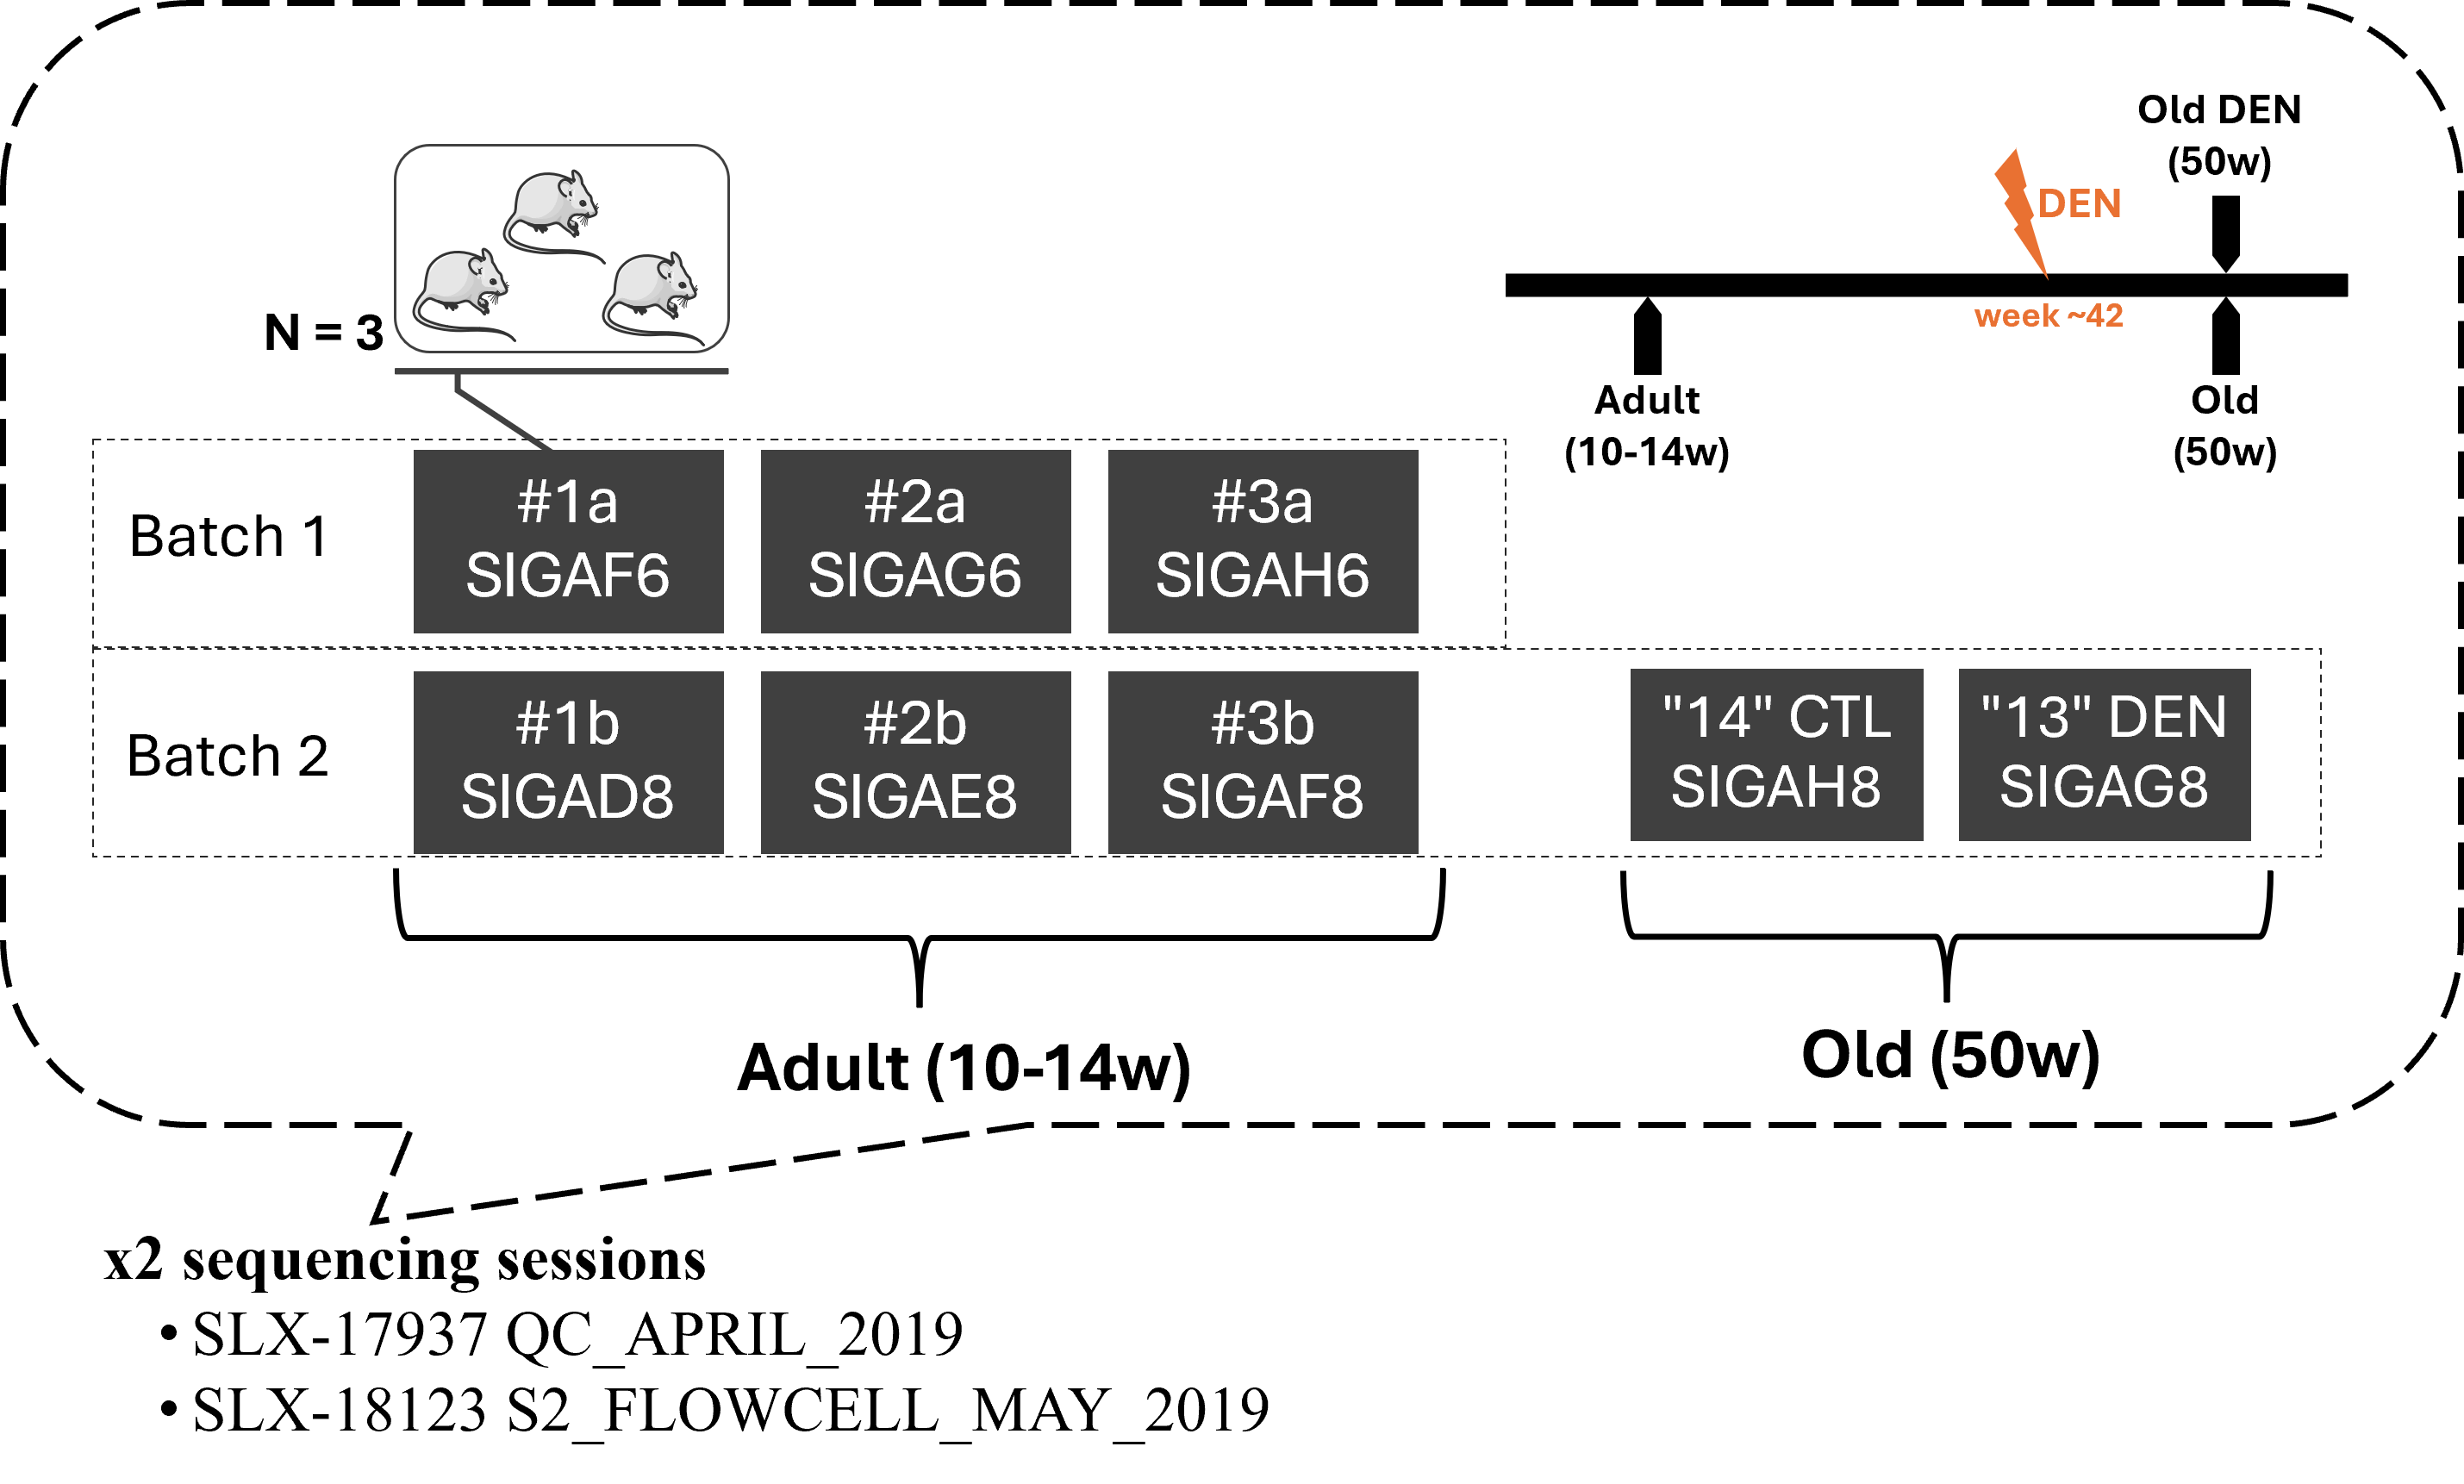
\includegraphics{index_files/mediabag/library_design_mouse.png}

}

\caption{Library design}

\end{figure}%%
\begin{figure}[H]

{\centering 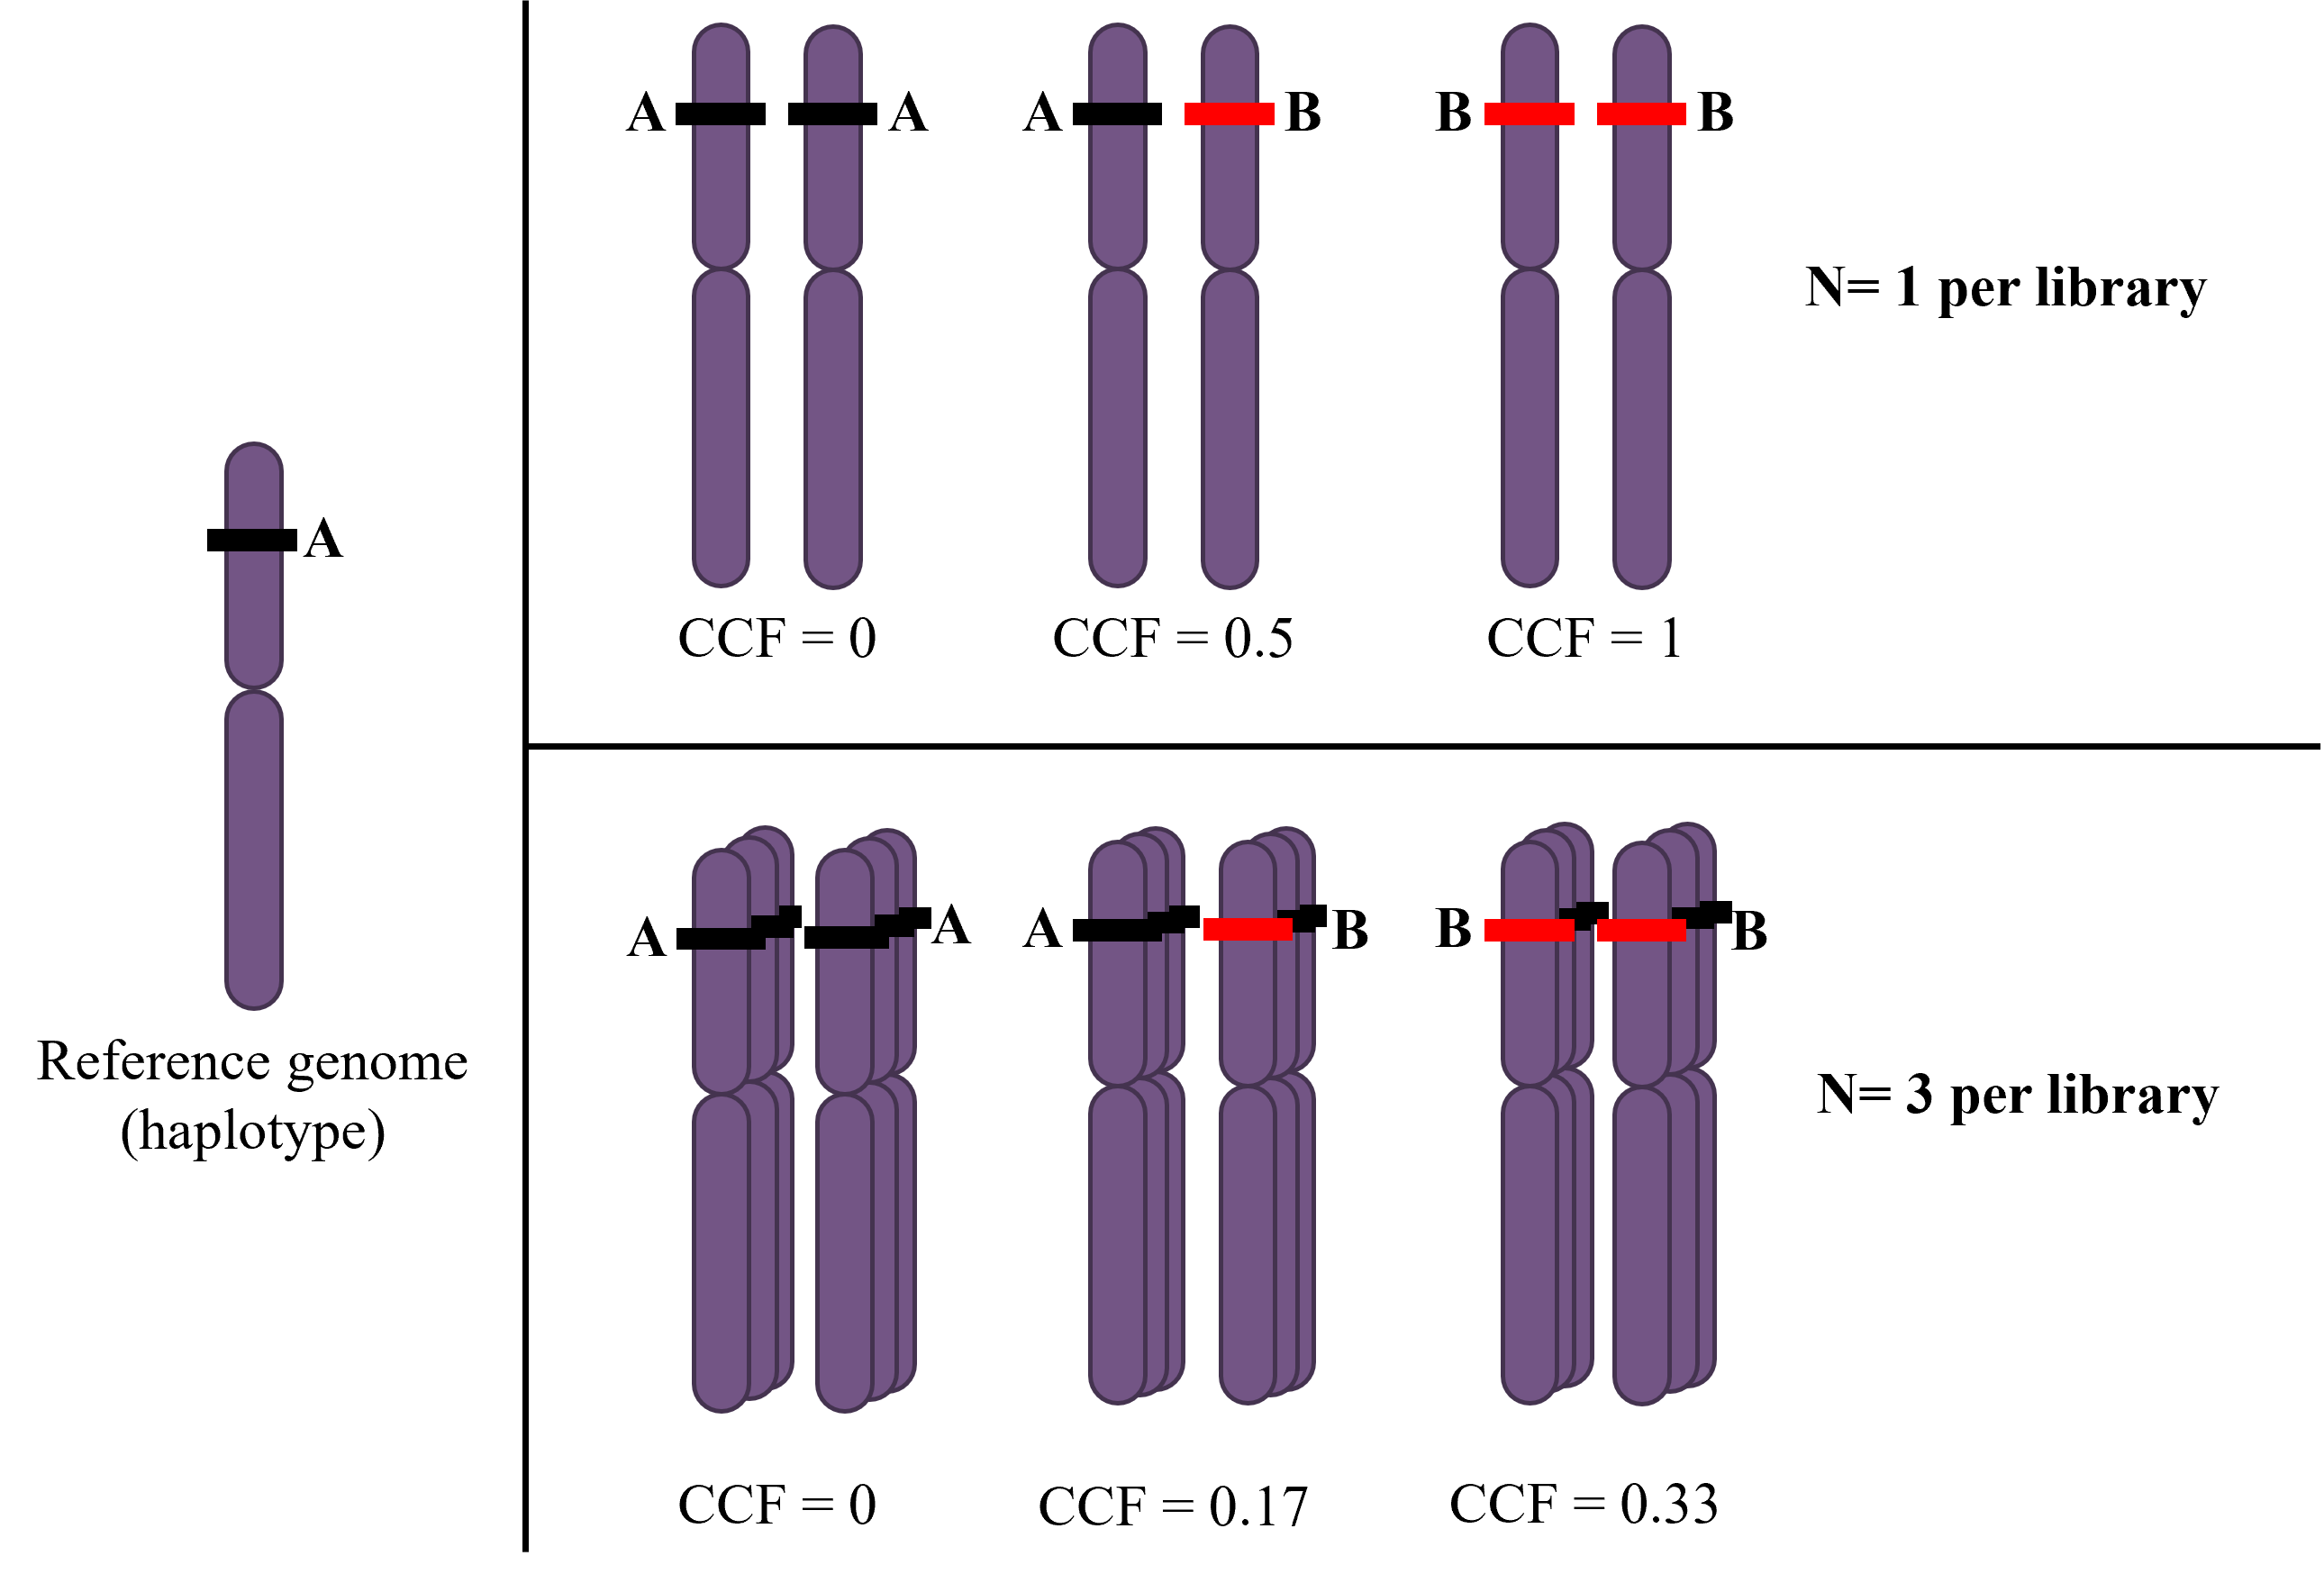
\includegraphics{index_files/mediabag/CCF_mouse.png}

}

\caption{Cancer cell fraction relation}

\end{figure}%

\subsection{Save cell barcodes with cell types in TSV format
(SComatic)}\label{save-cell-barcodes-with-cell-types-in-tsv-format-scomatic}

For SComatic, save cell barcodes with cell types: (first column is
barcode and second column is cell type)

\begin{Shaded}
\begin{Highlighting}[]
\CommentTok{\# colnames \textless{}{-} c("Index","Cell\_type")}

\CommentTok{\#df \textless{}{-} data.frame(Index = Cells(Esoph\_filt), Cell\_type = Esoph\_filt@meta.data$cellType)}

\CommentTok{\# delete suffix??}
\CommentTok{\# df$"Index" \textless{}{-} sapply(strsplit(df$"Index", "{-}"), \textasciigrave{}[\textasciigrave{}, 1)}

\CommentTok{\# write.table(df, file = \textquotesingle{}./output/esoph\_celltype.tsv\textquotesingle{}, col.names = TRUE, row.names = FALSE, sep = \textquotesingle{}\textbackslash{}t\textquotesingle{})}
\end{Highlighting}
\end{Shaded}

\section{Annotation of clusters (based on known canonical markers of
each
cluster)}\label{annotation-of-clusters-based-on-known-canonical-markers-of-each-cluster}

Annotate each mouse .tsv ``Cell\_type'' as: Epi; so that in Step 3 of
SComatic we obtain a .tsv with 1 ``cluster''

\begin{Shaded}
\begin{Highlighting}[]
 \DocumentationTok{\#\# Rearrange cluster order to follow differentiation axis (for visualization purposes) \# 9 clusters}
\FunctionTok{levels}\NormalTok{(Esoph\_filt) }\OtherTok{\textless{}{-}} \FunctionTok{c}\NormalTok{(}\DecValTok{2}\NormalTok{,}\DecValTok{4}\NormalTok{,}\DecValTok{1}\NormalTok{,}\DecValTok{3}\NormalTok{,}\DecValTok{5}\NormalTok{) }\CommentTok{\# from less differentiated to most (basal to luminal)}

\CommentTok{\# we have 5 clusters in Esoph\_filt}
\CommentTok{\# now, we want to just annotate Epi (all the cells in our Esoph\_filt are Epithelial)}
\NormalTok{new.cluster.id }\OtherTok{\textless{}{-}} \FunctionTok{c}\NormalTok{(}\StringTok{"Epi"}\NormalTok{, }\StringTok{"Epi"}\NormalTok{, }\StringTok{"Epi"}\NormalTok{, }\StringTok{"Epi"}\NormalTok{, }\StringTok{"Epi"}\NormalTok{)}

\FunctionTok{names}\NormalTok{(new.cluster.id) }\OtherTok{\textless{}{-}} \FunctionTok{levels}\NormalTok{(Esoph\_filt)}
\NormalTok{Esoph\_filt }\OtherTok{\textless{}{-}} \FunctionTok{RenameIdents}\NormalTok{(Esoph\_filt, new.cluster.id)}

\NormalTok{Esoph\_filt[[}\StringTok{"cellType"}\NormalTok{]] }\OtherTok{\textless{}{-}} \FunctionTok{Idents}\NormalTok{(Esoph\_filt) }\CommentTok{\# include it in the metadata}

\CommentTok{\# Create a new meta.data column named cellType\_B that adds \_lib1 if the library\_ID is llib1, and adds \_lib4 if the Library\_ID is lib2}
\NormalTok{Esoph\_filt}\SpecialCharTok{$}\NormalTok{cellType\_B }\OtherTok{\textless{}{-}} \FunctionTok{paste0}\NormalTok{(Esoph\_filt}\SpecialCharTok{$}\NormalTok{Library\_ID, }\StringTok{"\_"}\NormalTok{, Esoph\_filt}\SpecialCharTok{$}\NormalTok{cellType)}
\NormalTok{Esoph\_filt}\SpecialCharTok{$}\NormalTok{cellType\_B }\OtherTok{\textless{}{-}} \FunctionTok{as.factor}\NormalTok{(Esoph\_filt}\SpecialCharTok{$}\NormalTok{cellType\_B)}
\end{Highlighting}
\end{Shaded}

\begin{Shaded}
\begin{Highlighting}[]
\CommentTok{\# Get the unique sample IDs}
\NormalTok{sample\_names }\OtherTok{\textless{}{-}} \FunctionTok{unique}\NormalTok{(Esoph\_filt}\SpecialCharTok{@}\NormalTok{meta.data}\SpecialCharTok{$}\NormalTok{Sample\_name)}

\CommentTok{\# Create the .tsv files for each sample (we will have 16 different tsv files, one for each .bam)}
\NormalTok{tsv\_file }\OtherTok{\textless{}{-}} \ControlFlowTok{function}\NormalTok{(seurat\_obj, sample\_names) \{}
  \ControlFlowTok{for}\NormalTok{ (sample }\ControlFlowTok{in}\NormalTok{ sample\_names) \{}
    \CommentTok{\# Filter the data for the current sample}
\NormalTok{    sample\_data }\OtherTok{\textless{}{-}}\NormalTok{ seurat\_obj}\SpecialCharTok{@}\NormalTok{meta.data }\SpecialCharTok{\%\textgreater{}\%}
      \FunctionTok{filter}\NormalTok{(Sample\_name }\SpecialCharTok{==}\NormalTok{ sample)}
    
    \CommentTok{\# Add the Index column with the correct rownames and apply the transformation}
\NormalTok{    sample\_data}\SpecialCharTok{$}\NormalTok{Index }\OtherTok{\textless{}{-}} \FunctionTok{sapply}\NormalTok{(}\FunctionTok{strsplit}\NormalTok{(}\FunctionTok{rownames}\NormalTok{(sample\_data), }\StringTok{"{-}"}\NormalTok{), }\StringTok{\textasciigrave{}}\AttributeTok{[}\StringTok{\textasciigrave{}}\NormalTok{, }\DecValTok{1}\NormalTok{)}
    
    \CommentTok{\# Select the required columns}
\NormalTok{    sample\_data }\OtherTok{\textless{}{-}}\NormalTok{ sample\_data }\SpecialCharTok{\%\textgreater{}\%}
      \FunctionTok{select}\NormalTok{(Index, }\AttributeTok{Cell\_type =}\NormalTok{ cellType\_B) }\CommentTok{\# Cell\_type is a meta.data feature like "cellType\_B"}
    
    \CommentTok{\# Define the file name}
\NormalTok{    sample\_parts }\OtherTok{\textless{}{-}} \FunctionTok{strsplit}\NormalTok{(sample, }\StringTok{"\_"}\NormalTok{)[[}\DecValTok{1}\NormalTok{]]}
\NormalTok{    file\_name }\OtherTok{\textless{}{-}} \FunctionTok{paste0}\NormalTok{(}\StringTok{"./output/esoph\_markers\_scomatic\_"}\NormalTok{, sample\_parts[}\DecValTok{2}\NormalTok{], }\StringTok{"\_"}\NormalTok{, sample\_parts[}\DecValTok{1}\NormalTok{], }\StringTok{".tsv"}\NormalTok{)}
    
    \CommentTok{\# Write the data to a .tsv file}
    \FunctionTok{write.table}\NormalTok{(sample\_data, }\AttributeTok{file =}\NormalTok{ file\_name, }\AttributeTok{sep =} \StringTok{"}\SpecialCharTok{\textbackslash{}t}\StringTok{"}\NormalTok{, }\AttributeTok{row.names =} \ConstantTok{FALSE}\NormalTok{, }\AttributeTok{col.names =} \ConstantTok{TRUE}\NormalTok{, }\AttributeTok{quote =} \ConstantTok{FALSE}\NormalTok{)}
\NormalTok{  \}}
\NormalTok{\}}

\FunctionTok{tsv\_file}\NormalTok{(Esoph\_filt, sample\_names)}
\end{Highlighting}
\end{Shaded}

\begin{Shaded}
\begin{Highlighting}[]
\CommentTok{\# Check if we have taken all the rows:}
\NormalTok{output\_dir }\OtherTok{\textless{}{-}} \StringTok{"./output/"}

\CommentTok{\# Get a list of all .tsv files in the directory}
\NormalTok{tsv\_files }\OtherTok{\textless{}{-}} \FunctionTok{list.files}\NormalTok{(}\AttributeTok{path =}\NormalTok{ output\_dir, }\AttributeTok{pattern =} \StringTok{"\^{}esoph\_markers\_scomatic\_.*}\SpecialCharTok{\textbackslash{}\textbackslash{}}\StringTok{.tsv$"}\NormalTok{, }\AttributeTok{full.names =} \ConstantTok{TRUE}\NormalTok{)}

\CommentTok{\# Initialize a data frame to store the file names and row counts}
\NormalTok{row\_counts }\OtherTok{\textless{}{-}} \FunctionTok{data.frame}\NormalTok{(}\AttributeTok{File =} \FunctionTok{character}\NormalTok{(), }\AttributeTok{Rows =} \FunctionTok{integer}\NormalTok{(), }\AttributeTok{stringsAsFactors =} \ConstantTok{FALSE}\NormalTok{)}

\CommentTok{\# Loop through each file, read the data, and count the rows}
\ControlFlowTok{for}\NormalTok{ (file }\ControlFlowTok{in}\NormalTok{ tsv\_files) \{}
  \CommentTok{\# Read the data from the .tsv file}
\NormalTok{  data }\OtherTok{\textless{}{-}} \FunctionTok{read.table}\NormalTok{(file, }\AttributeTok{sep =} \StringTok{"}\SpecialCharTok{\textbackslash{}t}\StringTok{"}\NormalTok{, }\AttributeTok{header =} \ConstantTok{TRUE}\NormalTok{)}
  
  \CommentTok{\# Get the number of rows}
\NormalTok{  num\_rows }\OtherTok{\textless{}{-}} \FunctionTok{nrow}\NormalTok{(data)}
  
  \CommentTok{\# Add the file name and row count to the data frame}
\NormalTok{  row\_counts }\OtherTok{\textless{}{-}}\NormalTok{ row\_counts }\SpecialCharTok{\%\textgreater{}\%}
    \FunctionTok{add\_row}\NormalTok{(}\AttributeTok{File =} \FunctionTok{basename}\NormalTok{(file), }\AttributeTok{Rows =}\NormalTok{ num\_rows)}
\NormalTok{\}}

\NormalTok{total\_rows }\OtherTok{\textless{}{-}} \FunctionTok{sum}\NormalTok{(row\_counts}\SpecialCharTok{$}\NormalTok{Rows)}
\NormalTok{total\_rows}

\FunctionTok{dim}\NormalTok{(Esoph\_filt)}
\end{Highlighting}
\end{Shaded}

\section{scVelo preparation}\label{scvelo-preparation}

\subsection{Cluster annotation for
scvelo}\label{cluster-annotation-for-scvelo}

Looking at our umap, with resolution 0.2, we will take 3 clusters
(Basal, Suprabasal, Epi\_DEN), but annotated differently, in 5 names: -
Cluster 1: ``Basal 1'' - Cluster 2: ``Basal 2'' - Cluster 3:
``Suprabasal'' - Cluster 4: ``Basal 3'' - Cluster 5: ``Epithelial\_DEN''

\begin{Shaded}
\begin{Highlighting}[]
\FunctionTok{DimPlot}\NormalTok{(Esoph\_filt, }\AttributeTok{group.by =} \StringTok{"SCT\_snn\_res.0.2"}\NormalTok{) }\SpecialCharTok{\&}\NormalTok{ palette\_d}
\end{Highlighting}
\end{Shaded}

\begin{Shaded}
\begin{Highlighting}[]
\CommentTok{\# make sure we are using the idents we want right now:}
\FunctionTok{Idents}\NormalTok{(Esoph\_filt) }\OtherTok{\textless{}{-}}\NormalTok{ Esoph\_filt}\SpecialCharTok{$}\NormalTok{SCT\_snn\_res.}\FloatTok{0.2}
\NormalTok{Esoph\_filt}\SpecialCharTok{$}\NormalTok{seurat\_clusters }\OtherTok{\textless{}{-}}\NormalTok{ Esoph\_filt}\SpecialCharTok{$}\NormalTok{SCT\_snn\_res.}\FloatTok{0.2}

\DocumentationTok{\#\# Rearrange cluster order to follow differentiation axis (for visualization purposes) }
\FunctionTok{levels}\NormalTok{(Esoph\_filt) }\OtherTok{\textless{}{-}} \FunctionTok{c}\NormalTok{(}\DecValTok{1}\NormalTok{, }\DecValTok{2}\NormalTok{, }\DecValTok{4}\NormalTok{, }\DecValTok{3}\NormalTok{, }\DecValTok{5}\NormalTok{) }\CommentTok{\# from less differentiated to most (basal to luminal)}
\CommentTok{\# clusters 1 2 and 4 are basal (red, orange and blue)}
\CommentTok{\# cluster 3 (green) is suprabasal}
\CommentTok{\# cluster 5 is specific of condition sample\_DEN }

\NormalTok{new.cluster.ids }\OtherTok{\textless{}{-}} \FunctionTok{c}\NormalTok{(}\StringTok{"Basal\_1"}\NormalTok{, }\StringTok{"Basal\_2"}\NormalTok{, }\StringTok{"Basal\_3"}\NormalTok{, }\StringTok{"Suprabasal"}\NormalTok{, }\StringTok{"Epithelial\_DEN"}\NormalTok{) }\CommentTok{\# 1, 2, 4, 3, 5}
\FunctionTok{names}\NormalTok{(new.cluster.ids) }\OtherTok{\textless{}{-}} \FunctionTok{levels}\NormalTok{(Esoph\_filt)}
\NormalTok{Esoph\_filt }\OtherTok{\textless{}{-}} \FunctionTok{RenameIdents}\NormalTok{(Esoph\_filt, new.cluster.ids)}
\end{Highlighting}
\end{Shaded}

\begin{Shaded}
\begin{Highlighting}[]
\FunctionTok{Idents}\NormalTok{(Esoph\_filt) }\OtherTok{\textless{}{-}}\NormalTok{ Esoph\_filt}\SpecialCharTok{$}\NormalTok{annot\_scvelo}

\CommentTok{\# Annotated PCA and UMAP plots:}
\FunctionTok{DimPlot}\NormalTok{(Esoph\_filt, }\AttributeTok{reduction =} \StringTok{"pca"}\NormalTok{, }\AttributeTok{label =} \ConstantTok{TRUE}\NormalTok{, }\AttributeTok{pt.size =} \FloatTok{0.5}\NormalTok{) }\SpecialCharTok{+} \FunctionTok{NoLegend}\NormalTok{() }\SpecialCharTok{\&}\NormalTok{ palette\_d}

\FunctionTok{DimPlot}\NormalTok{(Esoph\_filt, }\AttributeTok{reduction =} \StringTok{"umap"}\NormalTok{, }\AttributeTok{label =} \ConstantTok{TRUE}\NormalTok{, }\AttributeTok{pt.size =} \FloatTok{0.5}\NormalTok{) }\SpecialCharTok{\&}\NormalTok{ palette\_d}
\end{Highlighting}
\end{Shaded}

\begin{Shaded}
\begin{Highlighting}[]
\FunctionTok{DimPlot}\NormalTok{(Esoph\_filt, }\AttributeTok{reduction =} \StringTok{"umap"}\NormalTok{, }\AttributeTok{label =} \ConstantTok{TRUE}\NormalTok{, }\AttributeTok{pt.size =} \FloatTok{0.5}\NormalTok{, }\AttributeTok{split.by =} \StringTok{"condition"}\NormalTok{) }\SpecialCharTok{\&}\NormalTok{ palette\_d}
\end{Highlighting}
\end{Shaded}

\begin{Shaded}
\begin{Highlighting}[]
\DocumentationTok{\#\# Remaining annotation using top markers for every cluster compared to all remaining ones, reporting only the positive ones}
\NormalTok{Esoph\_filt.markers }\OtherTok{\textless{}{-}} \FunctionTok{FindAllMarkers}\NormalTok{(Esoph\_filt, }\AttributeTok{only.pos =} \ConstantTok{TRUE}\NormalTok{, }\AttributeTok{min.pct =} \FloatTok{0.25}\NormalTok{, }\AttributeTok{logfc.threshold =} \FloatTok{0.25}\NormalTok{) }\CommentTok{\# restrict to features with a min of 0.25 logFC}
\CommentTok{\# write.table(Esoph\_filt.markers, file = \textquotesingle{}./output/Esoph\_markers\_filt.txt\textquotesingle{}, col.names = TRUE, row.names = TRUE, sep = \textquotesingle{}\textbackslash{}t\textquotesingle{})}
\NormalTok{Esoph\_filt.markers }\OtherTok{\textless{}{-}} \FunctionTok{read.csv}\NormalTok{(}\StringTok{"./output/Esoph\_markers\_filt.txt"}\NormalTok{, }\AttributeTok{sep =} \StringTok{"}\SpecialCharTok{\textbackslash{}t}\StringTok{"}\NormalTok{)}

\NormalTok{TopMarkers }\OtherTok{\textless{}{-}}\NormalTok{ Esoph\_filt.markers }\SpecialCharTok{\%\textgreater{}\%} \FunctionTok{group\_by}\NormalTok{(cluster) }\SpecialCharTok{\%\textgreater{}\%} \FunctionTok{top\_n}\NormalTok{(}\AttributeTok{n =} \DecValTok{25}\NormalTok{, }\AttributeTok{wt =}\NormalTok{ avg\_log2FC) }\CommentTok{\# show just top 25 per cluster}

\NormalTok{TopMarkers }\SpecialCharTok{\%\textgreater{}\%} \FunctionTok{write.csv}\NormalTok{(}\StringTok{"/home/albax/mcGinn\_2021/output/Esoph\_TopMarkers.csv"}\NormalTok{)}
\NormalTok{clusterB1\_markers }\OtherTok{\textless{}{-}}\NormalTok{ TopMarkers[TopMarkers}\SpecialCharTok{$}\NormalTok{cluster }\SpecialCharTok{==} \StringTok{"Basal\_1"}\NormalTok{, ]  }\CommentTok{\# Basal\_1}
\NormalTok{clusterB2\_markers }\OtherTok{\textless{}{-}}\NormalTok{ TopMarkers[TopMarkers}\SpecialCharTok{$}\NormalTok{cluster }\SpecialCharTok{==} \StringTok{"Basal\_2"}\NormalTok{, ]  }\CommentTok{\# Basal\_2}
\NormalTok{clusterB3\_markers }\OtherTok{\textless{}{-}}\NormalTok{ TopMarkers[TopMarkers}\SpecialCharTok{$}\NormalTok{cluster }\SpecialCharTok{==} \StringTok{"Basal\_3"}\NormalTok{, ]  }\CommentTok{\# Basal\_3}
\NormalTok{clusterSB\_markers }\OtherTok{\textless{}{-}}\NormalTok{ TopMarkers[TopMarkers}\SpecialCharTok{$}\NormalTok{cluster }\SpecialCharTok{==} \StringTok{"Suprabasal"}\NormalTok{, ]  }\CommentTok{\# Suprabasal}
\NormalTok{clusterEpDEN\_markers }\OtherTok{\textless{}{-}}\NormalTok{ TopMarkers[TopMarkers}\SpecialCharTok{$}\NormalTok{cluster }\SpecialCharTok{==} \StringTok{"Epithelial\_DEN"}\NormalTok{, ]  }\CommentTok{\# Epithelial\_DEN}
\end{Highlighting}
\end{Shaded}

\begin{Shaded}
\begin{Highlighting}[]
\NormalTok{Esoph\_filt.markers }\OtherTok{\textless{}{-}} \FunctionTok{read.csv}\NormalTok{(}\StringTok{"./output/Esoph\_markers\_clusts.txt"}\NormalTok{, }\AttributeTok{sep =} \StringTok{"}\SpecialCharTok{\textbackslash{}t}\StringTok{"}\NormalTok{)}

\NormalTok{TopMarkers }\OtherTok{\textless{}{-}}\NormalTok{ Esoph\_filt.markers }\SpecialCharTok{\%\textgreater{}\%} \FunctionTok{group\_by}\NormalTok{(cluster) }\SpecialCharTok{\%\textgreater{}\%} \FunctionTok{top\_n}\NormalTok{(}\AttributeTok{n =} \DecValTok{25}\NormalTok{, }\AttributeTok{wt =}\NormalTok{ avg\_log2FC) }\CommentTok{\# show just top 25 per cluster}

\NormalTok{B1\_markers }\OtherTok{\textless{}{-}}\NormalTok{ TopMarkers[TopMarkers}\SpecialCharTok{$}\NormalTok{cluster }\SpecialCharTok{==} \StringTok{\textquotesingle{}Basal\_1\textquotesingle{}}\NormalTok{, ]}
\NormalTok{B2\_markers }\OtherTok{\textless{}{-}}\NormalTok{ TopMarkers[TopMarkers}\SpecialCharTok{$}\NormalTok{cluster }\SpecialCharTok{==} \StringTok{\textquotesingle{}Basal\_2\textquotesingle{}}\NormalTok{, ]}
\NormalTok{B3\_markers }\OtherTok{\textless{}{-}}\NormalTok{ TopMarkers[TopMarkers}\SpecialCharTok{$}\NormalTok{cluster }\SpecialCharTok{==} \StringTok{\textquotesingle{}Basal\_3\textquotesingle{}}\NormalTok{, ]}
\NormalTok{DEN\_markers }\OtherTok{\textless{}{-}}\NormalTok{ TopMarkers[TopMarkers}\SpecialCharTok{$}\NormalTok{cluster }\SpecialCharTok{==} \StringTok{\textquotesingle{}Epithelial\_DEN\textquotesingle{}}\NormalTok{, ]}
\NormalTok{suprabasal\_markers }\OtherTok{\textless{}{-}}\NormalTok{ TopMarkers[TopMarkers}\SpecialCharTok{$}\NormalTok{cluster }\SpecialCharTok{==} \StringTok{\textquotesingle{}Suprabasal\textquotesingle{}}\NormalTok{, ]}
\end{Highlighting}
\end{Shaded}

\subsection{Conversion into h5ad object (export to
scvelo)}\label{conversion-into-h5ad-object-export-to-scvelo}

\begin{Shaded}
\begin{Highlighting}[]
\FunctionTok{.libPaths}\NormalTok{(}\StringTok{"/home/albax/miniforge3/envs/seuratdisk/lib/R/library"}\NormalTok{)}

\CommentTok{\# Esoph\_filt@meta.data$annot\_scvelo \textless{}{-} as.factor(Esoph\_filt@meta.data$annot\_scvelo)}

\FunctionTok{library}\NormalTok{(SeuratDisk) }\CommentTok{\# facilitates conversion between h5Seurat and AnnData objects, i.e. interoperability between Seurat and Scanpy}

\CommentTok{\# Make RNA assay (raw counts, which is a copy of spliced assay) default:}
\FunctionTok{DefaultAssay}\NormalTok{(Esoph\_filt) }\OtherTok{\textless{}{-}} \StringTok{"RNA"}

\NormalTok{remove\_scaledata }\OtherTok{\textless{}{-}} \ControlFlowTok{function}\NormalTok{(assay) \{}
\NormalTok{    assay}\SpecialCharTok{@}\NormalTok{scale.data }\OtherTok{\textless{}{-}} \FunctionTok{matrix}\NormalTok{(}\AttributeTok{nrow =} \DecValTok{0}\NormalTok{, }\AttributeTok{ncol =} \DecValTok{0}\NormalTok{)}
    \FunctionTok{return}\NormalTok{(assay)}
\NormalTok{\}}

\NormalTok{counts\_to\_integer }\OtherTok{\textless{}{-}} \ControlFlowTok{function}\NormalTok{(assay) \{}
\NormalTok{    assay}\SpecialCharTok{@}\NormalTok{counts}\SpecialCharTok{@}\NormalTok{x }\OtherTok{\textless{}{-}} \FunctionTok{as.integer}\NormalTok{(assay}\SpecialCharTok{@}\NormalTok{counts}\SpecialCharTok{@}\NormalTok{x)}
    \FunctionTok{return}\NormalTok{(assay)}
\NormalTok{\}}

\NormalTok{remove\_normalization }\OtherTok{\textless{}{-}} \ControlFlowTok{function}\NormalTok{(assay) \{}
\NormalTok{    assay}\SpecialCharTok{@}\NormalTok{data }\OtherTok{\textless{}{-}}\NormalTok{ assay}\SpecialCharTok{@}\NormalTok{counts}
    \FunctionTok{return}\NormalTok{(assay)}
\NormalTok{\}}

\NormalTok{Esoph\_filt}\SpecialCharTok{@}\NormalTok{assays }\OtherTok{\textless{}{-}} \FunctionTok{lapply}\NormalTok{(Esoph\_filt}\SpecialCharTok{@}\NormalTok{assays, remove\_scaledata)}
\NormalTok{Esoph\_filt}\SpecialCharTok{@}\NormalTok{assays }\OtherTok{\textless{}{-}} \FunctionTok{lapply}\NormalTok{(Esoph\_filt}\SpecialCharTok{@}\NormalTok{assays, counts\_to\_integer)}
\NormalTok{Esoph\_filt}\SpecialCharTok{@}\NormalTok{assays }\OtherTok{\textless{}{-}} \FunctionTok{lapply}\NormalTok{(Esoph\_filt}\SpecialCharTok{@}\NormalTok{assays, remove\_normalization)}

\CommentTok{\# Add a new metadata column so that cell types are stored as strings, and not as numbers in the anndata}
\NormalTok{Esoph\_filt}\SpecialCharTok{@}\NormalTok{meta.data}\SpecialCharTok{$}\NormalTok{annot\_scvelo\_names }\OtherTok{\textless{}{-}} \FunctionTok{as.character}\NormalTok{(Esoph\_filt}\SpecialCharTok{@}\NormalTok{meta.data}\SpecialCharTok{$}\NormalTok{annot\_scvelo)}

\CommentTok{\# File conversion:}
\FunctionTok{SaveH5Seurat}\NormalTok{(Esoph\_filt, }\AttributeTok{filename =} \StringTok{"Esoph.h5Seurat"}\NormalTok{, }\AttributeTok{overwrite=}\ConstantTok{TRUE}\NormalTok{)}
\FunctionTok{Convert}\NormalTok{(}\StringTok{"Esoph.h5Seurat"}\NormalTok{, }\AttributeTok{dest =} \StringTok{"h5ad"}\NormalTok{, }\AttributeTok{overwrite=}\ConstantTok{TRUE}\NormalTok{)}
\end{Highlighting}
\end{Shaded}

Save seurat object:

\begin{Shaded}
\begin{Highlighting}[]
\FunctionTok{saveRDS}\NormalTok{(Esoph\_filt, }\AttributeTok{file =} \StringTok{"./output/esoph\_star\_filtered\_mm10.rds"}\NormalTok{)}
\end{Highlighting}
\end{Shaded}

\section{Normalization of counts}\label{normalization-of-counts}

We are going to normalize the data by total counts (in each
library-Sequencing ID). For that, we have to sum all the columns.

\begin{Shaded}
\begin{Highlighting}[]
\FunctionTok{levels}\NormalTok{(Esoph\_filt}\SpecialCharTok{@}\NormalTok{meta.data}\SpecialCharTok{$}\NormalTok{Sample\_name)}
\FunctionTok{summary}\NormalTok{(Esoph\_filt[,Esoph\_filt}\SpecialCharTok{@}\NormalTok{meta.data}\SpecialCharTok{$}\NormalTok{Sample\_name }\SpecialCharTok{==} \StringTok{\textquotesingle{}lib2\_run1\textquotesingle{}}\NormalTok{]}\SpecialCharTok{@}\NormalTok{meta.data}\SpecialCharTok{$}\NormalTok{Sample\_name)}

\NormalTok{results\_df }\OtherTok{\textless{}{-}} \FunctionTok{data.frame}\NormalTok{(}\AttributeTok{Sample\_name =} \FunctionTok{character}\NormalTok{(), }\AttributeTok{Sum\_nCount\_gene =} \FunctionTok{numeric}\NormalTok{(), }\AttributeTok{Sum\_nFeature\_gene =} \FunctionTok{numeric}\NormalTok{(), }\AttributeTok{stringsAsFactors =} \ConstantTok{FALSE}\NormalTok{)}
\NormalTok{cell\_counts\_per\_sample }\OtherTok{\textless{}{-}} \FunctionTok{table}\NormalTok{(Esoph\_filt}\SpecialCharTok{@}\NormalTok{meta.data}\SpecialCharTok{$}\NormalTok{Sample\_name) }\CommentTok{\# number of cells per sample\_name}
 
\CommentTok{\# suma de los nCount\_gene para cada Sample\_name}
\ControlFlowTok{for}\NormalTok{ (i }\ControlFlowTok{in} \FunctionTok{unique}\NormalTok{(Esoph\_filt}\SpecialCharTok{$}\NormalTok{Sample\_name)) \{}
  \CommentTok{\# Subset the data based on the current sample name and calculate the sum of nCount\_gene}
\NormalTok{  sum\_count }\OtherTok{\textless{}{-}} \FunctionTok{sum}\NormalTok{(Esoph\_filt[, Esoph\_filt}\SpecialCharTok{$}\NormalTok{Sample\_name }\SpecialCharTok{==}\NormalTok{ i]}\SpecialCharTok{$}\NormalTok{nCount\_gene)}
\NormalTok{  sum\_feature }\OtherTok{\textless{}{-}} \FunctionTok{sum}\NormalTok{(Esoph\_filt[, Esoph\_filt}\SpecialCharTok{$}\NormalTok{Sample\_name }\SpecialCharTok{==}\NormalTok{ i]}\SpecialCharTok{$}\NormalTok{nFeature\_gene)}
\NormalTok{  num\_cells }\OtherTok{\textless{}{-}}\NormalTok{ cell\_counts\_per\_sample[i]}

  \CommentTok{\# Append the results to the results\_df}
\NormalTok{  results\_df }\OtherTok{\textless{}{-}} \FunctionTok{rbind}\NormalTok{(results\_df, }\FunctionTok{data.frame}\NormalTok{(}\AttributeTok{Sample\_name =}\NormalTok{ i, }\AttributeTok{Sum\_nCount\_gene =}\NormalTok{ sum\_count, }\AttributeTok{Num\_cells =}\NormalTok{ num\_cells, }\AttributeTok{Sum\_nFeature\_gene =}\NormalTok{ sum\_feature, }\AttributeTok{Num\_reads\_per\_cell =}\NormalTok{ sum\_count}\SpecialCharTok{/}\NormalTok{num\_cells, }\AttributeTok{Num\_genes\_per\_cell =}\NormalTok{ sum\_feature}\SpecialCharTok{/}\NormalTok{num\_cells ))}
\NormalTok{\}}
\NormalTok{numeric\_medians }\OtherTok{\textless{}{-}} \FunctionTok{apply}\NormalTok{(results\_df[, }\SpecialCharTok{{-}}\DecValTok{1}\NormalTok{], }\DecValTok{2}\NormalTok{, median)}
\NormalTok{median\_row }\OtherTok{\textless{}{-}} \FunctionTok{c}\NormalTok{(}\AttributeTok{Sample\_name =} \StringTok{"Median"}\NormalTok{, numeric\_medians)}
\NormalTok{results\_df }\OtherTok{\textless{}{-}} \FunctionTok{rbind}\NormalTok{(results\_df, median\_row)}

\FunctionTok{write.csv}\NormalTok{(results\_df, }\StringTok{"nCounts\_per\_Sample\_name\_Esophfilt.csv"}\NormalTok{, }\AttributeTok{row.names =} \ConstantTok{FALSE}\NormalTok{)}
\end{Highlighting}
\end{Shaded}

\textbf{Supplementary table from the original paper} nCount total is
going to ve similar to column 4 * column 6

Supplementary Table 1 - QC Statistics of scRNAseq data
(https://www.nature.com/articles/s41556-021-00679-w\#Sec31)

\begin{longtable}[]{@{}
  >{\raggedright\arraybackslash}p{(\columnwidth - 14\tabcolsep) * \real{0.0486}}
  >{\raggedright\arraybackslash}p{(\columnwidth - 14\tabcolsep) * \real{0.1111}}
  >{\raggedright\arraybackslash}p{(\columnwidth - 14\tabcolsep) * \real{0.0764}}
  >{\raggedright\arraybackslash}p{(\columnwidth - 14\tabcolsep) * \real{0.1250}}
  >{\raggedright\arraybackslash}p{(\columnwidth - 14\tabcolsep) * \real{0.1389}}
  >{\raggedright\arraybackslash}p{(\columnwidth - 14\tabcolsep) * \real{0.1319}}
  >{\raggedright\arraybackslash}p{(\columnwidth - 14\tabcolsep) * \real{0.1667}}
  >{\raggedright\arraybackslash}p{(\columnwidth - 14\tabcolsep) * \real{0.2014}}@{}}
\toprule\noalign{}
\begin{minipage}[b]{\linewidth}\raggedright
Stage
\end{minipage} & \begin{minipage}[b]{\linewidth}\raggedright
Replicate no.
\end{minipage} & \begin{minipage}[b]{\linewidth}\raggedright
Batch no.
\end{minipage} & \begin{minipage}[b]{\linewidth}\raggedright
Number of cells
\end{minipage} & \begin{minipage}[b]{\linewidth}\raggedright
Median genes/cell
\end{minipage} & \begin{minipage}[b]{\linewidth}\raggedright
Median UMIs/cell
\end{minipage} & \begin{minipage}[b]{\linewidth}\raggedright
Total genes detected
\end{minipage} & \begin{minipage}[b]{\linewidth}\raggedright
Median \% mito counts/cell
\end{minipage} \\
\midrule\noalign{}
\endhead
\bottomrule\noalign{}
\endlastfoot
Adult & 1 & 1 & 2796 & 5153 & 30737 & 17419 & 3.66549437744719 \\
Adult & 2 & 1 & 3344 & 5232 & 32745.5 & 17574 & 3.76114454638533 \\
Adult & 3 & 1 & 4059 & 5070 & 29744 & 17843 & 4.14769410907473 \\
Adult & 1 & 2 & 1230 & 5215 & 33187.5 & 16440 & 3.63571622273852 \\
Adult & 2 & 2 & 2614 & 5219 & 33970 & 17191 & 3.25793271016975 \\
Adult & 3 & 2 & \emph{676} & 5438 & \emph{36246.5} & 15707 &
3.5389684657119 \\
\end{longtable}

\begin{tcolorbox}[enhanced jigsaw, toprule=.15mm, left=2mm, arc=.35mm, rightrule=.15mm, breakable, bottomrule=.15mm, colframe=quarto-callout-warning-color-frame, leftrule=.75mm, colback=white, opacityback=0]

\vspace{-3mm}\textbf{Warning:}\vspace{3mm}

SCTransform corrects the counts from your equivalent RNA assay and
creates a new assay (typically SCT) where the counts slot is a corrected
counts, data is a log transformation of corrected counts+1 and the
scale.data are pearson residuals. Typically, the scale.data slot is only
generated for the features listed in VariableFeatures(your\_object)
which is why it's usually smaller than your SCT data slot. You can tell
SCTransform to scale all genes, but whether that's something you need or
not is up to you.

\end{tcolorbox}

\section{Do we find barcodes from Epi\_DEN shared in other
clusters?}\label{do-we-find-barcodes-from-epi_den-shared-in-other-clusters}

\begin{itemize}
\tightlist
\item
  Is each clone contained completely inside the Epithelial\_DEN
  cluster?(``Epi\_DEN\_cells'')
\item
  How are these clones shared with other clusters? How many cells of the
  clone fall inside Epi\_DEN\_cells cluster?
\item
\end{itemize}

\begin{Shaded}
\begin{Highlighting}[]
\NormalTok{epi\_den\_CBs }\OtherTok{\textless{}{-}} \FunctionTok{WhichCells}\NormalTok{(Esoph\_filt, }\AttributeTok{idents =} \StringTok{"Epithelial\_DEN"}\NormalTok{)}
\FunctionTok{write.csv}\NormalTok{(epi\_den\_CBs, }\StringTok{"Epithelial\_DEN\_CBS.txt"}\NormalTok{, }\AttributeTok{row.names =} \ConstantTok{FALSE}\NormalTok{)}

\NormalTok{metadata }\OtherTok{\textless{}{-}} \FunctionTok{data.frame}\NormalTok{(Esoph\_filt}\SpecialCharTok{@}\NormalTok{meta.data)}
\NormalTok{metadata\_cols }\OtherTok{\textless{}{-}}\NormalTok{ metadata[,}\FunctionTok{c}\NormalTok{(}\StringTok{"clones"}\NormalTok{, }\StringTok{"annot\_scvelo"}\NormalTok{), drop }\OtherTok{=} \ConstantTok{FALSE}\NormalTok{]}
\FunctionTok{write.csv}\NormalTok{(metadata\_cols, }\StringTok{"clones\_clusters.csv"}\NormalTok{, }\AttributeTok{row.names =} \ConstantTok{TRUE}\NormalTok{)}

\NormalTok{clones\_data }\OtherTok{\textless{}{-}}\NormalTok{ metadata[epi\_den\_CBs, }\FunctionTok{c}\NormalTok{(}\StringTok{"clones"}\NormalTok{, }\StringTok{"annot\_scvelo"}\NormalTok{), drop }\OtherTok{=} \ConstantTok{FALSE}\NormalTok{]}

\NormalTok{clones\_in\_Epi\_DEN }\OtherTok{\textless{}{-}} \FunctionTok{as.character}\NormalTok{(clones\_data[[}\StringTok{"clones"}\NormalTok{]])}
\NormalTok{clones\_in\_Epi\_DEN }\OtherTok{\textless{}{-}} \FunctionTok{unique}\NormalTok{(}\FunctionTok{unlist}\NormalTok{(}\FunctionTok{strsplit}\NormalTok{(clones\_in\_Epi\_DEN, }\StringTok{","}\NormalTok{)))}
\end{Highlighting}
\end{Shaded}

\chapter{3. Inference of velocity}\label{inference-of-velocity}

\section{Slingshot}\label{slingshot}

\begin{Shaded}
\begin{Highlighting}[]
\FunctionTok{.libPaths}\NormalTok{(}\StringTok{"/home/albax/miniforge3/envs/seurat\_v4/lib/R/library"}\NormalTok{)}

\FunctionTok{library}\NormalTok{(Seurat)}
\FunctionTok{library}\NormalTok{(slingshot)}

\FunctionTok{library}\NormalTok{(grDevices)}
\FunctionTok{library}\NormalTok{(RColorBrewer)}
\FunctionTok{library}\NormalTok{(ggplot2)}
\FunctionTok{library}\NormalTok{(dplyr)}
\FunctionTok{library}\NormalTok{(viridis)}
\end{Highlighting}
\end{Shaded}

\subsection{Load filtered seurat
object}\label{load-filtered-seurat-object}

\begin{Shaded}
\begin{Highlighting}[]
\NormalTok{Esoph }\OtherTok{\textless{}{-}} \FunctionTok{readRDS}\NormalTok{(}\AttributeTok{file =} \StringTok{"mcGinn\_2021/output/esoph\_star\_filtered\_mm10.rds"}\NormalTok{)}

\CommentTok{\# Convert SeuratObject to SingleCellExperiment with Seurat function \textquotesingle{}as.SingleCellExperiment()\textquotesingle{}}
\NormalTok{Esoph\_sce }\OtherTok{\textless{}{-}} \FunctionTok{as.SingleCellExperiment}\NormalTok{(Esoph)}

\CommentTok{\# view idents}
\FunctionTok{Idents}\NormalTok{(Esoph) }\CommentTok{\# Basal\_1, Basal\_2, Basal\_3, Suprabasal, Epithelial\_DEN}

\CommentTok{\# view metadata columns from sce experiment object, in order to know which one to use }
\NormalTok{Esoph\_sce}\SpecialCharTok{@}\NormalTok{colData}

\CommentTok{\# we will use annot\_scvelo which has 5 levels: Basal\_1, Basal\_2, Basal\_3, Suprabasal, Epithelial\_DEN}
\NormalTok{Esoph\_sce}\SpecialCharTok{@}\NormalTok{colData}\SpecialCharTok{$}\NormalTok{annot\_scvelo}

\CommentTok{\# add umap data to sce object}
\NormalTok{umap\_data }\OtherTok{\textless{}{-}} \FunctionTok{Embeddings}\NormalTok{(Esoph[[}\StringTok{"umap"}\NormalTok{]])  }\CommentTok{\# Extract UMAP data}
\FunctionTok{reducedDims}\NormalTok{(Esoph\_sce)}\SpecialCharTok{$}\NormalTok{UMAP }\OtherTok{\textless{}{-}}\NormalTok{ umap\_data}

\FunctionTok{factor}\NormalTok{(Esoph\_sce}\SpecialCharTok{$}\NormalTok{annot\_scvelo)}
\end{Highlighting}
\end{Shaded}

\begin{Shaded}
\begin{Highlighting}[]
\CommentTok{\# Run trajectory inference with slingshot}
\FunctionTok{set.seed}\NormalTok{(}\DecValTok{1}\NormalTok{)}
\NormalTok{Esoph\_sce }\OtherTok{\textless{}{-}} \FunctionTok{slingshot}\NormalTok{(Esoph\_sce, }\AttributeTok{clusterLabels =} \StringTok{\textquotesingle{}annot\_scvelo\textquotesingle{}}\NormalTok{, }\AttributeTok{reducedDim =} \StringTok{\textquotesingle{}UMAP\textquotesingle{}}\NormalTok{)}
\NormalTok{Esoph\_sce}\SpecialCharTok{$}\NormalTok{slingParams[}\StringTok{"star.clus"}\NormalTok{]}
\NormalTok{Esoph\_sce}\SpecialCharTok{$}\NormalTok{slingParams[}\StringTok{"end.clus"}\NormalTok{]}

\NormalTok{slingshot\_obj }\OtherTok{\textless{}{-}} \FunctionTok{SlingshotDataSet}\NormalTok{(Esoph\_sce)}
\NormalTok{slingshot\_obj}\SpecialCharTok{@}\NormalTok{slingParams}\SpecialCharTok{$}\NormalTok{start.clus}
\NormalTok{slingshot\_obj}\SpecialCharTok{@}\NormalTok{slingParams}\SpecialCharTok{$}\NormalTok{end.clus}
\end{Highlighting}
\end{Shaded}

\subsection{Plot results}\label{plot-results}

\begin{Shaded}
\begin{Highlighting}[]
\CommentTok{\# Plot trajectory (curves how they are called by Slingshot)}
\FunctionTok{png}\NormalTok{(}\StringTok{"slingshot\_results/plots/Esoph\_slingshot\_mm10.png"}\NormalTok{, }\AttributeTok{width=}\DecValTok{1000}\NormalTok{, }\AttributeTok{height=}\DecValTok{1000}\NormalTok{, }\AttributeTok{units=}\StringTok{"px"}\NormalTok{)}

\NormalTok{breaks }\OtherTok{\textless{}{-}} \FunctionTok{seq}\NormalTok{(}\FunctionTok{min}\NormalTok{(}\FunctionTok{slingPseudotime}\NormalTok{(Esoph\_sce, }\AttributeTok{na=}\ConstantTok{FALSE}\NormalTok{), }\AttributeTok{na.rm =} \ConstantTok{TRUE}\NormalTok{), }
               \FunctionTok{max}\NormalTok{(}\FunctionTok{slingPseudotime}\NormalTok{(Esoph\_sce, }\AttributeTok{na=}\ConstantTok{FALSE}\NormalTok{), }\AttributeTok{na.rm =} \ConstantTok{TRUE}\NormalTok{), }
               \AttributeTok{length.out =} \DecValTok{100}\NormalTok{)}
\NormalTok{viridis\_colors }\OtherTok{\textless{}{-}} \FunctionTok{magma}\NormalTok{(}\DecValTok{100}\NormalTok{)}
\NormalTok{plotcol }\OtherTok{\textless{}{-}}\NormalTok{ viridis\_colors[}\FunctionTok{cut}\NormalTok{(}\FunctionTok{slingPseudotime}\NormalTok{(Esoph\_sce, }\AttributeTok{na=}\ConstantTok{FALSE}\NormalTok{), }\AttributeTok{breaks =}\NormalTok{ breaks)]}

\FunctionTok{layout}\NormalTok{(}\FunctionTok{matrix}\NormalTok{(}\FunctionTok{c}\NormalTok{(}\DecValTok{1}\NormalTok{, }\DecValTok{2}\NormalTok{), }\AttributeTok{ncol =} \DecValTok{2}\NormalTok{), }\AttributeTok{widths =} \FunctionTok{c}\NormalTok{(}\DecValTok{2}\NormalTok{, }\FloatTok{0.25}\NormalTok{), }\AttributeTok{height =} \FunctionTok{c}\NormalTok{(}\DecValTok{1}\NormalTok{,}\FloatTok{0.2}\NormalTok{))}
\FunctionTok{par}\NormalTok{(}\AttributeTok{mar=}\FunctionTok{c}\NormalTok{(}\DecValTok{5}\NormalTok{, }\DecValTok{4}\NormalTok{, }\DecValTok{4}\NormalTok{, }\DecValTok{1}\NormalTok{), }\AttributeTok{xpd=}\ConstantTok{TRUE}\NormalTok{)  }\CommentTok{\# Adjust margins for the main plot}
\FunctionTok{plot}\NormalTok{(}\FunctionTok{reducedDims}\NormalTok{(Esoph\_sce)}\SpecialCharTok{$}\NormalTok{UMAP, }\AttributeTok{col =}\NormalTok{ plotcol, }\AttributeTok{pch=}\DecValTok{16}\NormalTok{, }\AttributeTok{asp =} \DecValTok{1}\NormalTok{)}

\FunctionTok{lines}\NormalTok{(}\FunctionTok{SlingshotDataSet}\NormalTok{(Esoph\_sce), }\AttributeTok{lwd=}\DecValTok{2}\NormalTok{, }\AttributeTok{col=}\StringTok{\textquotesingle{}black\textquotesingle{}}\NormalTok{)}
\FunctionTok{lines}\NormalTok{(}\FunctionTok{SlingshotDataSet}\NormalTok{(Esoph\_sce), }\AttributeTok{type =} \StringTok{\textquotesingle{}lineages\textquotesingle{}}\NormalTok{, }\AttributeTok{lwd=}\DecValTok{2}\NormalTok{, }\AttributeTok{col=}\StringTok{\textquotesingle{}black\textquotesingle{}}\NormalTok{)}

\FunctionTok{par}\NormalTok{(}\AttributeTok{mar =} \FunctionTok{c}\NormalTok{(}\DecValTok{5}\NormalTok{, }\DecValTok{1}\NormalTok{, }\DecValTok{4}\NormalTok{, }\DecValTok{1}\NormalTok{)) }
\FunctionTok{plot.new}\NormalTok{() }
\FunctionTok{plot.window}\NormalTok{(}\AttributeTok{xlim =} \FunctionTok{c}\NormalTok{(}\DecValTok{0}\NormalTok{, }\DecValTok{1}\NormalTok{), }\AttributeTok{ylim =} \FunctionTok{c}\NormalTok{(}\DecValTok{0}\NormalTok{, }\DecValTok{1}\NormalTok{))}

\NormalTok{legend\_image }\OtherTok{\textless{}{-}} \FunctionTok{as.raster}\NormalTok{(viridis\_colors, }\AttributeTok{ncol=}\DecValTok{1}\NormalTok{)}
\NormalTok{legend\_width }\OtherTok{\textless{}{-}} \FloatTok{0.7}
\NormalTok{legend\_height }\OtherTok{\textless{}{-}} \FloatTok{0.25}
\NormalTok{x\_left }\OtherTok{\textless{}{-}}\NormalTok{ (}\DecValTok{1} \SpecialCharTok{{-}}\NormalTok{ legend\_width) }\SpecialCharTok{/} \DecValTok{2}
\NormalTok{x\_right }\OtherTok{\textless{}{-}}\NormalTok{ x\_left }\SpecialCharTok{+}\NormalTok{ legend\_width}
\NormalTok{y\_bottom }\OtherTok{\textless{}{-}}\NormalTok{ (}\DecValTok{1} \SpecialCharTok{{-}}\NormalTok{ legend\_height) }\SpecialCharTok{/} \DecValTok{2}
\NormalTok{y\_top }\OtherTok{\textless{}{-}}\NormalTok{ y\_bottom }\SpecialCharTok{+}\NormalTok{ legend\_height}
\FunctionTok{rasterImage}\NormalTok{(legend\_image, x\_left, y\_bottom, x\_right, y\_top)}
\FunctionTok{text}\NormalTok{(}\AttributeTok{x =} \FloatTok{0.5}\NormalTok{, }\AttributeTok{y =} \FloatTok{0.65}\NormalTok{, }\AttributeTok{labels =} \StringTok{"Legend"}\NormalTok{, }\AttributeTok{cex =} \FloatTok{1.2}\NormalTok{, }\AttributeTok{font =} \DecValTok{2}\NormalTok{, }\AttributeTok{pos =} \DecValTok{3}\NormalTok{)}

\FunctionTok{dev.off}\NormalTok{()}
\end{Highlighting}
\end{Shaded}

\begin{Shaded}
\begin{Highlighting}[]
\CommentTok{\# Plot trajectory (curves how they are called by Slingshot)}
\FunctionTok{png}\NormalTok{(}\StringTok{"slingshot\_results/plots/Esoph\_slingshot\_curves\_mm10.png"}\NormalTok{, }\AttributeTok{width=}\DecValTok{1000}\NormalTok{, }\AttributeTok{height=}\DecValTok{1000}\NormalTok{, }\AttributeTok{units=}\StringTok{"px"}\NormalTok{)}

\NormalTok{breaks }\OtherTok{\textless{}{-}} \FunctionTok{seq}\NormalTok{(}\FunctionTok{min}\NormalTok{(}\FunctionTok{slingPseudotime}\NormalTok{(Esoph\_sce, }\AttributeTok{na=}\ConstantTok{FALSE}\NormalTok{), }\AttributeTok{na.rm =} \ConstantTok{TRUE}\NormalTok{), }
               \FunctionTok{max}\NormalTok{(}\FunctionTok{slingPseudotime}\NormalTok{(Esoph\_sce, }\AttributeTok{na=}\ConstantTok{FALSE}\NormalTok{), }\AttributeTok{na.rm =} \ConstantTok{TRUE}\NormalTok{), }
               \AttributeTok{length.out =} \DecValTok{100}\NormalTok{)}
\NormalTok{viridis\_colors }\OtherTok{\textless{}{-}} \FunctionTok{magma}\NormalTok{(}\DecValTok{100}\NormalTok{)}
\NormalTok{plotcol }\OtherTok{\textless{}{-}}\NormalTok{ viridis\_colors[}\FunctionTok{cut}\NormalTok{(}\FunctionTok{slingPseudotime}\NormalTok{(Esoph\_sce, }\AttributeTok{na=}\ConstantTok{FALSE}\NormalTok{), }\AttributeTok{breaks =}\NormalTok{ breaks)]}

\FunctionTok{layout}\NormalTok{(}\FunctionTok{matrix}\NormalTok{(}\FunctionTok{c}\NormalTok{(}\DecValTok{1}\NormalTok{, }\DecValTok{2}\NormalTok{), }\AttributeTok{ncol =} \DecValTok{2}\NormalTok{), }\AttributeTok{widths =} \FunctionTok{c}\NormalTok{(}\DecValTok{2}\NormalTok{, }\FloatTok{0.25}\NormalTok{), }\AttributeTok{height =} \FunctionTok{c}\NormalTok{(}\DecValTok{1}\NormalTok{,}\FloatTok{0.2}\NormalTok{))}
\FunctionTok{par}\NormalTok{(}\AttributeTok{mar=}\FunctionTok{c}\NormalTok{(}\DecValTok{5}\NormalTok{, }\DecValTok{4}\NormalTok{, }\DecValTok{4}\NormalTok{, }\DecValTok{1}\NormalTok{), }\AttributeTok{xpd=}\ConstantTok{TRUE}\NormalTok{)  }\CommentTok{\# Adjust margins for the main plot}
\FunctionTok{plot}\NormalTok{(}\FunctionTok{reducedDims}\NormalTok{(Esoph\_sce)}\SpecialCharTok{$}\NormalTok{UMAP, }\AttributeTok{col =}\NormalTok{ plotcol, }\AttributeTok{pch=}\DecValTok{16}\NormalTok{, }\AttributeTok{asp =} \DecValTok{1}\NormalTok{)}

\FunctionTok{lines}\NormalTok{(}\FunctionTok{SlingshotDataSet}\NormalTok{(Esoph\_sce), }\AttributeTok{lwd=}\DecValTok{2}\NormalTok{, }\AttributeTok{col=}\StringTok{\textquotesingle{}black\textquotesingle{}}\NormalTok{)}
\CommentTok{\# lines(SlingshotDataSet(Esoph\_sce), type = \textquotesingle{}lineages\textquotesingle{}, lwd=2, col=\textquotesingle{}black\textquotesingle{})}

\FunctionTok{par}\NormalTok{(}\AttributeTok{mar =} \FunctionTok{c}\NormalTok{(}\DecValTok{5}\NormalTok{, }\DecValTok{1}\NormalTok{, }\DecValTok{4}\NormalTok{, }\DecValTok{1}\NormalTok{)) }
\FunctionTok{plot.new}\NormalTok{() }
\FunctionTok{plot.window}\NormalTok{(}\AttributeTok{xlim =} \FunctionTok{c}\NormalTok{(}\DecValTok{0}\NormalTok{, }\DecValTok{1}\NormalTok{), }\AttributeTok{ylim =} \FunctionTok{c}\NormalTok{(}\DecValTok{0}\NormalTok{, }\DecValTok{1}\NormalTok{))}

\NormalTok{legend\_image }\OtherTok{\textless{}{-}} \FunctionTok{as.raster}\NormalTok{(viridis\_colors, }\AttributeTok{ncol=}\DecValTok{1}\NormalTok{)}
\NormalTok{legend\_width }\OtherTok{\textless{}{-}} \FloatTok{0.7}
\NormalTok{legend\_height }\OtherTok{\textless{}{-}} \FloatTok{0.25}
\NormalTok{x\_left }\OtherTok{\textless{}{-}}\NormalTok{ (}\DecValTok{1} \SpecialCharTok{{-}}\NormalTok{ legend\_width) }\SpecialCharTok{/} \DecValTok{2}
\NormalTok{x\_right }\OtherTok{\textless{}{-}}\NormalTok{ x\_left }\SpecialCharTok{+}\NormalTok{ legend\_width}
\NormalTok{y\_bottom }\OtherTok{\textless{}{-}}\NormalTok{ (}\DecValTok{1} \SpecialCharTok{{-}}\NormalTok{ legend\_height) }\SpecialCharTok{/} \DecValTok{2}
\NormalTok{y\_top }\OtherTok{\textless{}{-}}\NormalTok{ y\_bottom }\SpecialCharTok{+}\NormalTok{ legend\_height}
\FunctionTok{rasterImage}\NormalTok{(legend\_image, x\_left, y\_bottom, x\_right, y\_top)}
\FunctionTok{text}\NormalTok{(}\AttributeTok{x =} \FloatTok{0.5}\NormalTok{, }\AttributeTok{y =} \FloatTok{0.65}\NormalTok{, }\AttributeTok{labels =} \StringTok{"Legend"}\NormalTok{, }\AttributeTok{cex =} \FloatTok{1.2}\NormalTok{, }\AttributeTok{font =} \DecValTok{2}\NormalTok{, }\AttributeTok{pos =} \DecValTok{3}\NormalTok{)}

\FunctionTok{dev.off}\NormalTok{()}
\end{Highlighting}
\end{Shaded}

\subsection{Plot lineage structure}\label{plot-lineage-structure}

\begin{Shaded}
\begin{Highlighting}[]
\NormalTok{palette\_d }\OtherTok{\textless{}{-}} \FunctionTok{c}\NormalTok{(}\StringTok{"\#7A0403FF"}\NormalTok{, }\StringTok{"\#FB8022FF"}\NormalTok{, }\StringTok{"\#A2FC3CFF"}\NormalTok{, }\StringTok{"\#28BBECFF"}\NormalTok{, }\StringTok{"\#30123BFF"}\NormalTok{)}

\FunctionTok{png}\NormalTok{(}\StringTok{"./velocity/slingshot\_results/plots/Esoph\_slingshot\_trajectories\_clusters\_mm10.png"}\NormalTok{, }\AttributeTok{width=}\DecValTok{1000}\NormalTok{, }\AttributeTok{height=}\DecValTok{1000}\NormalTok{, }\AttributeTok{units=}\StringTok{"px"}\NormalTok{)}

\FunctionTok{plot}\NormalTok{(}\FunctionTok{reducedDims}\NormalTok{(Esoph\_sce)}\SpecialCharTok{$}\NormalTok{UMAP, }\AttributeTok{col =}\NormalTok{ palette\_d[}\FunctionTok{as.numeric}\NormalTok{(}\FunctionTok{droplevels}\NormalTok{(Esoph\_sce}\SpecialCharTok{$}\NormalTok{annot\_scvelo))], }\AttributeTok{pch=}\DecValTok{16}\NormalTok{, }\AttributeTok{asp =} \DecValTok{1}\NormalTok{)}

\FunctionTok{lines}\NormalTok{(}\FunctionTok{SlingshotDataSet}\NormalTok{(Esoph\_sce), }\AttributeTok{lwd=}\DecValTok{2}\NormalTok{, }\AttributeTok{type =} \StringTok{\textquotesingle{}lineages\textquotesingle{}}\NormalTok{, }\AttributeTok{col =} \StringTok{\textquotesingle{}black\textquotesingle{}}\NormalTok{)}

\FunctionTok{legend}\NormalTok{(}\AttributeTok{x=}\StringTok{"topright"}\NormalTok{, }\AttributeTok{legend=}\FunctionTok{c}\NormalTok{(}\StringTok{"Basal\_1"}\NormalTok{, }\StringTok{"Basal\_2"}\NormalTok{, }\StringTok{"Basal\_3"}\NormalTok{, }\StringTok{"Suprabasal"}\NormalTok{, }\StringTok{"Epithelial\_DEN"}\NormalTok{), }\AttributeTok{col=}\NormalTok{palette\_d[}\DecValTok{1}\SpecialCharTok{:}\DecValTok{5}\NormalTok{], }\AttributeTok{pch=}\DecValTok{16}\NormalTok{, }\AttributeTok{cex=}\DecValTok{2}\NormalTok{)}

\FunctionTok{dev.off}\NormalTok{()}
\end{Highlighting}
\end{Shaded}

\section{scVelo}\label{scvelo}

\subsection{Load of .h5ad file}\label{load-of-.h5ad-file}

\begin{Shaded}
\begin{Highlighting}[]
\CommentTok{\#!/home/albax/miniforge3/envs/ame python3}
\CommentTok{\# {-}*{-} coding: utf{-}8 {-}*{-}}
\CommentTok{"""}
\CommentTok{Created on Jul 26 2024}

\CommentTok{@author: albax}
\CommentTok{"""}
\ImportTok{import}\NormalTok{ sys}
\ImportTok{import}\NormalTok{ os}

\CommentTok{\# Add the site{-}packages directory to sys.path}
\NormalTok{specific\_path }\OperatorTok{=} \StringTok{"/home/albax/miniforge3/envs/ame/lib/python3.10/site{-}packages"}
\ControlFlowTok{if}\NormalTok{ specific\_path }\KeywordTok{not} \KeywordTok{in}\NormalTok{ sys.path:}
\NormalTok{    sys.path.append(specific\_path)}

\NormalTok{sys.path.insert(}\DecValTok{0}\NormalTok{, }\StringTok{\textquotesingle{}/home/albax/scvelo/scvelo\textquotesingle{}}\NormalTok{)}

\ImportTok{import}\NormalTok{ scvelo }\ImportTok{as}\NormalTok{ scv}
\ImportTok{import}\NormalTok{ scanpy }\ImportTok{as}\NormalTok{ sc}
\ImportTok{import}\NormalTok{ scipy.sparse }\ImportTok{as}\NormalTok{ sp}
\ImportTok{import}\NormalTok{ matplotlib.pyplot }\ImportTok{as}\NormalTok{ plt}
\ImportTok{import}\NormalTok{ seaborn }\ImportTok{as}\NormalTok{ sns}
\ImportTok{import}\NormalTok{ numpy }\ImportTok{as}\NormalTok{ np}
\ImportTok{from}\NormalTok{ matplotlib.colors }\ImportTok{import}\NormalTok{ ListedColormap}

\NormalTok{adata }\OperatorTok{=}\NormalTok{ scv.read(}\StringTok{"../Esoph.h5ad"}\NormalTok{, cache}\OperatorTok{=}\VariableTok{True}\NormalTok{)}

\NormalTok{adata}
\NormalTok{adata.layers.keys() }\CommentTok{\# should include spliced and unspliced}
\NormalTok{adata.layers[}\StringTok{\textquotesingle{}spliced\textquotesingle{}}\NormalTok{] }\CommentTok{\# check presence}
\NormalTok{adata.layers[}\StringTok{\textquotesingle{}unspliced\textquotesingle{}}\NormalTok{] }\CommentTok{\# check presence}
\NormalTok{adata.var\_names }\OperatorTok{=}\NormalTok{ adata.var[}\StringTok{\textquotesingle{}\_index\textquotesingle{}}\NormalTok{]}

\NormalTok{scv.pp.filter\_and\_normalize(adata, min\_shared\_counts}\OperatorTok{=}\DecValTok{20}\NormalTok{, n\_top\_genes}\OperatorTok{=}\DecValTok{2000}\NormalTok{)}

\CommentTok{\#\#\#\#\#\#\#\# deprecated: }
\CommentTok{\# scv.pp.moments(adata, n\_pcs=30, n\_neighbors=30)}
\CommentTok{\#\#\#\#\#\#\#\#\#\#\#\#\#\#\#\#}

\CommentTok{\# 2. Compute PCA with Scanpy}
\NormalTok{sc.pp.pca(adata, n\_comps}\OperatorTok{=}\DecValTok{30}\NormalTok{)}

\CommentTok{\# 2. Compute neighbors with Scanpy}
\NormalTok{sc.pp.neighbors(adata, n\_pcs}\OperatorTok{=}\DecValTok{30}\NormalTok{, n\_neighbors}\OperatorTok{=}\DecValTok{30}\NormalTok{, use\_rep}\OperatorTok{=}\StringTok{\textquotesingle{}X\_pca\textquotesingle{}}\NormalTok{)}

\NormalTok{scv.pp.moments(adata, n\_pcs}\OperatorTok{=}\DecValTok{30}\NormalTok{, n\_neighbors}\OperatorTok{=}\DecValTok{30}\NormalTok{) }\CommentTok{\# uses connectivites from step before}

\CommentTok{\# rename levels from annot\_scvelo slot}
\CommentTok{\# rename\_dict = \{}
\CommentTok{\#     0: \textquotesingle{}Basal\_1\textquotesingle{}, \# 1}
\CommentTok{\#     1: \textquotesingle{}Basal\_2\textquotesingle{}, \# 2}
\CommentTok{\#     2: \textquotesingle{}Basal\_3\textquotesingle{}, \# 3}
\CommentTok{\#     3: \textquotesingle{}Suprabasal\textquotesingle{}, \# 4}
\CommentTok{\#     4: \textquotesingle{}Epithelial\_DEN\textquotesingle{}, \# 5}
\CommentTok{\# \}}

\CommentTok{\# adata.obs[\textquotesingle{}annot\_scvelo\textquotesingle{}] = adata.obs[\textquotesingle{}annot\_scvelo\textquotesingle{}].replace(rename\_dict)}
\end{Highlighting}
\end{Shaded}

Define functions and colors for plotting:

\begin{Shaded}
\begin{Highlighting}[]
\KeywordTok{def}\NormalTok{ save\_stream(adata, }\BuiltInTok{file}\NormalTok{, }\BuiltInTok{format}\OperatorTok{=}\NormalTok{[}\StringTok{"svg"}\NormalTok{, }\StringTok{"png"}\NormalTok{], }\OperatorTok{**}\NormalTok{kwargs):}
\NormalTok{    fig, ax }\OperatorTok{=}\NormalTok{ plt.subplots(figsize}\OperatorTok{=}\NormalTok{(}\DecValTok{9}\NormalTok{, }\DecValTok{7}\NormalTok{))  }
\NormalTok{    scv.pl.velocity\_embedding\_stream(adata, ax}\OperatorTok{=}\NormalTok{ax, arrow\_size}\OperatorTok{=}\DecValTok{1}\NormalTok{, cutoff\_perc}\OperatorTok{=}\DecValTok{10}\NormalTok{, }\OperatorTok{**}\NormalTok{kwargs)}
    
    \ControlFlowTok{for}\NormalTok{ extension }\KeywordTok{in} \BuiltInTok{format}\NormalTok{:}
\NormalTok{        file\_name }\OperatorTok{=} \BuiltInTok{file} \OperatorTok{+} \StringTok{"."} \OperatorTok{+}\NormalTok{ extension}
\NormalTok{        fig.savefig(file\_name, }\BuiltInTok{format}\OperatorTok{=}\NormalTok{extension, bbox\_inches}\OperatorTok{=}\StringTok{\textquotesingle{}tight\textquotesingle{}}\NormalTok{)}
    
    \ControlFlowTok{return}\NormalTok{ fig, ax  }


\KeywordTok{def}\NormalTok{ save\_grid(adata, }\BuiltInTok{file}\NormalTok{, }\BuiltInTok{format}\OperatorTok{=}\NormalTok{[}\StringTok{"svg"}\NormalTok{, }\StringTok{"png"}\NormalTok{], }\OperatorTok{**}\NormalTok{kwargs):}
\NormalTok{    fig, ax }\OperatorTok{=}\NormalTok{ plt.subplots(figsize}\OperatorTok{=}\NormalTok{(}\DecValTok{9}\NormalTok{, }\DecValTok{7}\NormalTok{))  }
\NormalTok{    scv.pl.velocity\_embedding\_grid(adata, ax}\OperatorTok{=}\NormalTok{ax, arrow\_length}\OperatorTok{=}\DecValTok{5}\NormalTok{, arrow\_size}\OperatorTok{=}\DecValTok{3}\NormalTok{, }\OperatorTok{**}\NormalTok{kwargs) }

    \ControlFlowTok{for}\NormalTok{ extension }\KeywordTok{in} \BuiltInTok{format}\NormalTok{:}
\NormalTok{        file\_name }\OperatorTok{=} \BuiltInTok{file} \OperatorTok{+} \StringTok{"."} \OperatorTok{+}\NormalTok{ extension}
\NormalTok{        fig.savefig(file\_name, }\BuiltInTok{format}\OperatorTok{=}\NormalTok{extension, bbox\_inches}\OperatorTok{=}\StringTok{\textquotesingle{}tight\textquotesingle{}}\NormalTok{)}
    
    \ControlFlowTok{return}\NormalTok{ fig, ax }


\KeywordTok{def}\NormalTok{ save\_embedding(adata, }\BuiltInTok{file}\NormalTok{, }\BuiltInTok{format}\OperatorTok{=}\NormalTok{[}\StringTok{"svg"}\NormalTok{, }\StringTok{"png"}\NormalTok{], }\OperatorTok{**}\NormalTok{kwargs):}
\NormalTok{    fig, ax }\OperatorTok{=}\NormalTok{ plt.subplots(figsize}\OperatorTok{=}\NormalTok{(}\DecValTok{9}\NormalTok{, }\DecValTok{7}\NormalTok{)) }
\NormalTok{    scv.pl.velocity\_embedding(adata, ax}\OperatorTok{=}\NormalTok{ax, arrow\_length}\OperatorTok{=}\DecValTok{5}\NormalTok{, arrow\_size}\OperatorTok{=}\DecValTok{3}\NormalTok{, }\OperatorTok{**}\NormalTok{kwargs)  }
    
    \ControlFlowTok{for}\NormalTok{ extension }\KeywordTok{in} \BuiltInTok{format}\NormalTok{:}
\NormalTok{        file\_name }\OperatorTok{=} \BuiltInTok{file} \OperatorTok{+} \StringTok{"."} \OperatorTok{+}\NormalTok{ extension}
\NormalTok{        fig.savefig(file\_name, }\BuiltInTok{format}\OperatorTok{=}\NormalTok{extension, bbox\_inches}\OperatorTok{=}\StringTok{\textquotesingle{}tight\textquotesingle{}}\NormalTok{)}
    
    \ControlFlowTok{return}\NormalTok{ fig, ax  }


\NormalTok{palette }\OperatorTok{=}\NormalTok{ sns.color\_palette(}\StringTok{"plasma\_r"}\NormalTok{)}
\NormalTok{colors\_d }\OperatorTok{=}\NormalTok{ [}\StringTok{"\#7A0403FF"}\NormalTok{, }\StringTok{"\#FB8022FF"}\NormalTok{, }\StringTok{"\#A2FC3CFF"}\NormalTok{, }\StringTok{"\#30123BFF"}\NormalTok{, }\StringTok{"\#28BBECFF"}\NormalTok{]}
\NormalTok{palette\_d }\OperatorTok{=}\NormalTok{ sns.color\_palette(colors\_d)}
\end{Highlighting}
\end{Shaded}

\subsection{Stochastic model}\label{stochastic-model}

\begin{Shaded}
\begin{Highlighting}[]
\NormalTok{scv.tl.velocity(adata, mode }\OperatorTok{=}\StringTok{"stochastic"}\NormalTok{) }\CommentTok{\# not good model}
\NormalTok{scv.tl.velocity\_graph(adata, n\_jobs}\OperatorTok{=}\DecValTok{6}\NormalTok{) }\CommentTok{\# number of cores to use}

\CommentTok{\# scv.pl.pca(adata, color="annot\_scvelo")}
\CommentTok{\# scv.pl.umap(adata, color="annot\_scvelo")}
\end{Highlighting}
\end{Shaded}

\subsubsection{Save plots for stochastic
model}\label{save-plots-for-stochastic-model}

\begin{Shaded}
\begin{Highlighting}[]
\NormalTok{fig\_stream\_stoc, ax\_stream\_stoc }\OperatorTok{=}\NormalTok{ save\_stream(adata, }\BuiltInTok{file}\OperatorTok{=}\StringTok{"scvelo\_results/plots/Esoph\_stream\_stoch"}\NormalTok{, }\BuiltInTok{format}\OperatorTok{=}\NormalTok{[}\StringTok{\textquotesingle{}svg\textquotesingle{}}\NormalTok{, }\StringTok{\textquotesingle{}png\textquotesingle{}}\NormalTok{], basis}\OperatorTok{=}\StringTok{"umap"}\NormalTok{, color}\OperatorTok{=}\StringTok{"annot\_scvelo"}\NormalTok{, palette}\OperatorTok{=}\NormalTok{palette\_d, figsize}\OperatorTok{=}\NormalTok{(}\DecValTok{9}\NormalTok{, }\DecValTok{7}\NormalTok{), legend\_loc}\OperatorTok{=}\StringTok{\textquotesingle{}right margin\textquotesingle{}}\NormalTok{, title }\OperatorTok{=} \StringTok{"Stochastic model (stream)"}\NormalTok{)}

\NormalTok{fig\_grid\_stoc, ax\_grid\_stoc }\OperatorTok{=}\NormalTok{ save\_grid(adata, }\BuiltInTok{file}\OperatorTok{=}\StringTok{"scvelo\_results/plots/Esoph\_grid\_stoch"}\NormalTok{, }\BuiltInTok{format}\OperatorTok{=}\NormalTok{[}\StringTok{\textquotesingle{}svg\textquotesingle{}}\NormalTok{, }\StringTok{\textquotesingle{}png\textquotesingle{}}\NormalTok{], basis}\OperatorTok{=}\StringTok{\textquotesingle{}umap\textquotesingle{}}\NormalTok{, color}\OperatorTok{=}\StringTok{"annot\_scvelo"}\NormalTok{, palette}\OperatorTok{=}\NormalTok{palette\_d, figsize}\OperatorTok{=}\NormalTok{(}\DecValTok{9}\NormalTok{, }\DecValTok{7}\NormalTok{), legend\_loc}\OperatorTok{=}\StringTok{\textquotesingle{}right margin\textquotesingle{}}\NormalTok{, title }\OperatorTok{=} \StringTok{"Stochastic model (grid)"}\NormalTok{ )}

\NormalTok{fig\_embedding\_stoc, ax\_embedding\_stoc }\OperatorTok{=}\NormalTok{ save\_embedding(adata, }\BuiltInTok{file}\OperatorTok{=}\StringTok{"scvelo\_results/plots/Esoph\_veloc\_stoch"}\NormalTok{, }\BuiltInTok{format}\OperatorTok{=}\NormalTok{[}\StringTok{\textquotesingle{}svg\textquotesingle{}}\NormalTok{, }\StringTok{\textquotesingle{}png\textquotesingle{}}\NormalTok{], basis}\OperatorTok{=}\StringTok{"umap"}\NormalTok{, color}\OperatorTok{=}\StringTok{"annot\_scvelo"}\NormalTok{, palette}\OperatorTok{=}\NormalTok{palette\_d, figsize}\OperatorTok{=}\NormalTok{(}\DecValTok{9}\NormalTok{, }\DecValTok{7}\NormalTok{), legend\_loc}\OperatorTok{=}\StringTok{\textquotesingle{}right margin\textquotesingle{}}\NormalTok{, dpi}\OperatorTok{=}\DecValTok{200}\NormalTok{, title }\OperatorTok{=} \StringTok{"Stochastic model (embedding)"}\NormalTok{)}
\end{Highlighting}
\end{Shaded}

\begin{Shaded}
\begin{Highlighting}[]
\CommentTok{\# grid layout for stoc (run everything as chunk)}
\NormalTok{fig\_combined, axs }\OperatorTok{=}\NormalTok{ plt.subplots(}\DecValTok{1}\NormalTok{, }\DecValTok{3}\NormalTok{, figsize}\OperatorTok{=}\NormalTok{(}\DecValTok{27}\NormalTok{, }\DecValTok{7}\NormalTok{))}

\NormalTok{axs[}\DecValTok{0}\NormalTok{].imshow(fig\_stream\_stoc.canvas.renderer.buffer\_rgba())}
\NormalTok{axs[}\DecValTok{0}\NormalTok{].axis(}\StringTok{\textquotesingle{}off\textquotesingle{}}\NormalTok{)}
\NormalTok{axs[}\DecValTok{1}\NormalTok{].imshow(fig\_grid\_stoc.canvas.renderer.buffer\_rgba())}
\NormalTok{axs[}\DecValTok{1}\NormalTok{].axis(}\StringTok{\textquotesingle{}off\textquotesingle{}}\NormalTok{)}
\NormalTok{axs[}\DecValTok{2}\NormalTok{].imshow(fig\_embedding\_stoc.canvas.renderer.buffer\_rgba())}
\NormalTok{axs[}\DecValTok{2}\NormalTok{].axis(}\StringTok{\textquotesingle{}off\textquotesingle{}}\NormalTok{) }

\NormalTok{combined\_file\_path }\OperatorTok{=} \StringTok{"scvelo\_results/plots/Esoph\_combined\_plots\_stoc"}
\NormalTok{fig\_combined.tight\_layout()}
\NormalTok{fig\_combined.savefig(combined\_file\_path }\OperatorTok{+} \StringTok{\textquotesingle{}\_mm10.svg\textquotesingle{}}\NormalTok{, }\BuiltInTok{format}\OperatorTok{=}\StringTok{\textquotesingle{}svg\textquotesingle{}}\NormalTok{, bbox\_inches}\OperatorTok{=}\StringTok{\textquotesingle{}tight\textquotesingle{}}\NormalTok{)}
\NormalTok{fig\_combined.savefig(combined\_file\_path }\OperatorTok{+} \StringTok{\textquotesingle{}\_mm10.png\textquotesingle{}}\NormalTok{, }\BuiltInTok{format}\OperatorTok{=}\StringTok{\textquotesingle{}png\textquotesingle{}}\NormalTok{, dpi}\OperatorTok{=}\DecValTok{300}\NormalTok{, bbox\_inches}\OperatorTok{=}\StringTok{\textquotesingle{}tight\textquotesingle{}}\NormalTok{)}
\NormalTok{plt.show()}
\end{Highlighting}
\end{Shaded}

Save the .h5ad file with stochastic model

\begin{Shaded}
\begin{Highlighting}[]
\KeywordTok{del}\NormalTok{ adata.raw}
\NormalTok{adata.var.rename(columns}\OperatorTok{=}\NormalTok{\{}\StringTok{\textquotesingle{}\_index\textquotesingle{}}\NormalTok{: }\StringTok{\textquotesingle{}index\textquotesingle{}}\NormalTok{\}, inplace}\OperatorTok{=}\VariableTok{True}\NormalTok{)}
\NormalTok{adata.obs.rename(columns}\OperatorTok{=}\NormalTok{\{}\StringTok{\textquotesingle{}\_index\textquotesingle{}}\NormalTok{: }\StringTok{\textquotesingle{}index\textquotesingle{}}\NormalTok{\}, inplace}\OperatorTok{=}\VariableTok{True}\NormalTok{)}

\NormalTok{adata.write(filename }\OperatorTok{=} \StringTok{"scvelo\_results/Esoph\_stochastic\_mm10.h5ad"}\NormalTok{, compression}\OperatorTok{=}\StringTok{\textquotesingle{}gzip\textquotesingle{}}\NormalTok{)}
\end{Highlighting}
\end{Shaded}

\subsection{Deterministic model}\label{deterministic-model}

\begin{Shaded}
\begin{Highlighting}[]
\NormalTok{scv.tl.velocity(adata, mode }\OperatorTok{=} \StringTok{"deterministic"}\NormalTok{)}
\NormalTok{scv.tl.velocity\_graph(adata, n\_jobs}\OperatorTok{=}\DecValTok{6}\NormalTok{)}
\CommentTok{\# scv.pl.velocity\_embedding\_stream(adata, basis="umap", color="annot\_scvelo")}

\CommentTok{\# scv.pl.pca(adata, color="annot\_scvelo")}
\CommentTok{\# scv.pl.umap(adata, color="annot\_scvelo")}
\end{Highlighting}
\end{Shaded}

\subsubsection{Save plots of deterministic
model}\label{save-plots-of-deterministic-model}

\begin{Shaded}
\begin{Highlighting}[]
\NormalTok{fig\_stream\_det, ax\_stream\_det }\OperatorTok{=}\NormalTok{ save\_stream(adata, }\BuiltInTok{file}\OperatorTok{=}\StringTok{"scvelo\_results/plots/Esoph\_stream\_det"}\NormalTok{, }\BuiltInTok{format}\OperatorTok{=}\NormalTok{[}\StringTok{\textquotesingle{}svg\textquotesingle{}}\NormalTok{, }\StringTok{\textquotesingle{}png\textquotesingle{}}\NormalTok{], basis}\OperatorTok{=}\StringTok{"umap"}\NormalTok{, color}\OperatorTok{=}\StringTok{"annot\_scvelo"}\NormalTok{, palette}\OperatorTok{=}\NormalTok{palette\_d, figsize}\OperatorTok{=}\NormalTok{(}\DecValTok{9}\NormalTok{, }\DecValTok{7}\NormalTok{), legend\_loc}\OperatorTok{=}\StringTok{\textquotesingle{}right margin\textquotesingle{}}\NormalTok{, title }\OperatorTok{=} \StringTok{"Deterministic model (stream)"}\NormalTok{)}

\NormalTok{fig\_grid\_det, ax\_grid\_det }\OperatorTok{=}\NormalTok{ save\_grid(adata, }\BuiltInTok{file}\OperatorTok{=}\StringTok{"scvelo\_results/plots/Esoph\_grid\_det"}\NormalTok{, }\BuiltInTok{format}\OperatorTok{=}\NormalTok{[}\StringTok{\textquotesingle{}svg\textquotesingle{}}\NormalTok{, }\StringTok{\textquotesingle{}png\textquotesingle{}}\NormalTok{], basis}\OperatorTok{=}\StringTok{\textquotesingle{}umap\textquotesingle{}}\NormalTok{, color}\OperatorTok{=}\StringTok{"annot\_scvelo"}\NormalTok{, palette}\OperatorTok{=}\NormalTok{palette\_d, figsize}\OperatorTok{=}\NormalTok{(}\DecValTok{9}\NormalTok{, }\DecValTok{7}\NormalTok{), legend\_loc}\OperatorTok{=}\StringTok{\textquotesingle{}right margin\textquotesingle{}}\NormalTok{, title }\OperatorTok{=} \StringTok{"Deterministic model (grid)"}\NormalTok{ )}

\NormalTok{fig\_embedding\_det, ax\_embedding\_det }\OperatorTok{=}\NormalTok{ save\_embedding(adata, }\BuiltInTok{file}\OperatorTok{=}\StringTok{"scvelo\_results/plots/Esoph\_veloc\_det"}\NormalTok{, }\BuiltInTok{format}\OperatorTok{=}\NormalTok{[}\StringTok{\textquotesingle{}svg\textquotesingle{}}\NormalTok{, }\StringTok{\textquotesingle{}png\textquotesingle{}}\NormalTok{], basis}\OperatorTok{=}\StringTok{"umap"}\NormalTok{, color}\OperatorTok{=}\StringTok{"annot\_scvelo"}\NormalTok{, palette}\OperatorTok{=}\NormalTok{palette\_d, figsize}\OperatorTok{=}\NormalTok{(}\DecValTok{9}\NormalTok{, }\DecValTok{7}\NormalTok{), legend\_loc}\OperatorTok{=}\StringTok{\textquotesingle{}right margin\textquotesingle{}}\NormalTok{, dpi}\OperatorTok{=}\DecValTok{200}\NormalTok{, title }\OperatorTok{=} \StringTok{"Deterministic model (embedding)"}\NormalTok{)}
\end{Highlighting}
\end{Shaded}

\begin{Shaded}
\begin{Highlighting}[]
\CommentTok{\# grid layout for deterministic (run everything as chunk)}
\NormalTok{fig\_combined, axs }\OperatorTok{=}\NormalTok{ plt.subplots(}\DecValTok{1}\NormalTok{, }\DecValTok{3}\NormalTok{, figsize}\OperatorTok{=}\NormalTok{(}\DecValTok{27}\NormalTok{, }\DecValTok{7}\NormalTok{))}

\NormalTok{axs[}\DecValTok{0}\NormalTok{].imshow(fig\_stream\_det.canvas.renderer.buffer\_rgba())}
\NormalTok{axs[}\DecValTok{0}\NormalTok{].axis(}\StringTok{\textquotesingle{}off\textquotesingle{}}\NormalTok{)}
\NormalTok{axs[}\DecValTok{1}\NormalTok{].imshow(fig\_grid\_det.canvas.renderer.buffer\_rgba())}
\NormalTok{axs[}\DecValTok{1}\NormalTok{].axis(}\StringTok{\textquotesingle{}off\textquotesingle{}}\NormalTok{)}
\NormalTok{axs[}\DecValTok{2}\NormalTok{].imshow(fig\_embedding\_det.canvas.renderer.buffer\_rgba())}
\NormalTok{axs[}\DecValTok{2}\NormalTok{].axis(}\StringTok{\textquotesingle{}off\textquotesingle{}}\NormalTok{) }

\NormalTok{combined\_file\_path }\OperatorTok{=} \StringTok{"scvelo\_results/plots/Esoph\_combined\_plots\_det"}
\NormalTok{fig\_combined.tight\_layout()}
\NormalTok{fig\_combined.savefig(combined\_file\_path }\OperatorTok{+} \StringTok{\textquotesingle{}\_mm10.svg\textquotesingle{}}\NormalTok{, }\BuiltInTok{format}\OperatorTok{=}\StringTok{\textquotesingle{}svg\textquotesingle{}}\NormalTok{, bbox\_inches}\OperatorTok{=}\StringTok{\textquotesingle{}tight\textquotesingle{}}\NormalTok{)}
\NormalTok{fig\_combined.savefig(combined\_file\_path }\OperatorTok{+} \StringTok{\textquotesingle{}\_mm10.png\textquotesingle{}}\NormalTok{, }\BuiltInTok{format}\OperatorTok{=}\StringTok{\textquotesingle{}png\textquotesingle{}}\NormalTok{, dpi}\OperatorTok{=}\DecValTok{300}\NormalTok{, bbox\_inches}\OperatorTok{=}\StringTok{\textquotesingle{}tight\textquotesingle{}}\NormalTok{)}
\NormalTok{plt.show()}
\end{Highlighting}
\end{Shaded}

Save the .h5ad file with dererministic model

\begin{Shaded}
\begin{Highlighting}[]
\KeywordTok{del}\NormalTok{ adata.raw}
\NormalTok{adata.var.rename(columns}\OperatorTok{=}\NormalTok{\{}\StringTok{\textquotesingle{}\_index\textquotesingle{}}\NormalTok{: }\StringTok{\textquotesingle{}index\textquotesingle{}}\NormalTok{\}, inplace}\OperatorTok{=}\VariableTok{True}\NormalTok{)}
\NormalTok{adata.obs.rename(columns}\OperatorTok{=}\NormalTok{\{}\StringTok{\textquotesingle{}\_index\textquotesingle{}}\NormalTok{: }\StringTok{\textquotesingle{}index\textquotesingle{}}\NormalTok{\}, inplace}\OperatorTok{=}\VariableTok{True}\NormalTok{)}

\NormalTok{adata.write(filename }\OperatorTok{=} \StringTok{"scvelo\_results/Esoph\_deterministic\_mm10.h5ad"}\NormalTok{, compression}\OperatorTok{=}\StringTok{\textquotesingle{}gzip\textquotesingle{}}\NormalTok{)}
\end{Highlighting}
\end{Shaded}

\subsection{Dynamical model}\label{dynamical-model}

\begin{Shaded}
\begin{Highlighting}[]
\NormalTok{adata }\OperatorTok{=}\NormalTok{ adata[:, adata.var[}\StringTok{\textquotesingle{}highly\_variable\textquotesingle{}}\NormalTok{]]  }\CommentTok{\# Only use highly variable genes}
\NormalTok{scv.tl.recover\_dynamics(adata, n\_jobs}\OperatorTok{=}\DecValTok{6}\NormalTok{)}
\NormalTok{scv.tl.velocity(adata, mode }\OperatorTok{=} \StringTok{"dynamical"}\NormalTok{)}
\NormalTok{scv.tl.velocity\_graph(adata, n\_jobs}\OperatorTok{=}\DecValTok{6}\NormalTok{)}

\NormalTok{scv.pl.velocity\_embedding\_stream(adata, basis}\OperatorTok{=}\StringTok{"umap"}\NormalTok{, color}\OperatorTok{=}\StringTok{"annot\_scvelo\_names"}\NormalTok{)}

\CommentTok{\# scv.pl.pca(adata, color="annot\_scvelo")}
\CommentTok{\# scv.pl.umap(adata, color="annot\_scvelo")}
\end{Highlighting}
\end{Shaded}

\subsubsection{Save plots for dynamical
model}\label{save-plots-for-dynamical-model}

\begin{Shaded}
\begin{Highlighting}[]
\NormalTok{fig\_stream\_dyn, ax\_stream\_dyn }\OperatorTok{=}\NormalTok{ save\_stream(adata, }\BuiltInTok{file}\OperatorTok{=}\StringTok{"scvelo\_results/plots/Esoph\_stream\_dyn"}\NormalTok{, }\BuiltInTok{format}\OperatorTok{=}\NormalTok{[}\StringTok{\textquotesingle{}svg\textquotesingle{}}\NormalTok{, }\StringTok{\textquotesingle{}png\textquotesingle{}}\NormalTok{], basis}\OperatorTok{=}\StringTok{"umap"}\NormalTok{, color}\OperatorTok{=}\StringTok{"annot\_scvelo"}\NormalTok{, palette}\OperatorTok{=}\NormalTok{palette\_d, figsize}\OperatorTok{=}\NormalTok{(}\DecValTok{9}\NormalTok{, }\DecValTok{7}\NormalTok{), legend\_loc}\OperatorTok{=}\StringTok{\textquotesingle{}right margin\textquotesingle{}}\NormalTok{, title }\OperatorTok{=} \StringTok{"Dynamical model (stream)"}\NormalTok{)}

\NormalTok{fig\_grid\_dyn, ax\_grid\_dyn }\OperatorTok{=}\NormalTok{ save\_grid(adata, }\BuiltInTok{file}\OperatorTok{=}\StringTok{"scvelo\_results/plots/Esoph\_grid\_det"}\NormalTok{, }\BuiltInTok{format}\OperatorTok{=}\NormalTok{[}\StringTok{\textquotesingle{}svg\textquotesingle{}}\NormalTok{, }\StringTok{\textquotesingle{}png\textquotesingle{}}\NormalTok{], basis}\OperatorTok{=}\StringTok{\textquotesingle{}umap\textquotesingle{}}\NormalTok{, color}\OperatorTok{=}\StringTok{"annot\_scvelo"}\NormalTok{, palette}\OperatorTok{=}\NormalTok{palette\_d, figsize}\OperatorTok{=}\NormalTok{(}\DecValTok{9}\NormalTok{, }\DecValTok{7}\NormalTok{), legend\_loc}\OperatorTok{=}\StringTok{\textquotesingle{}right margin\textquotesingle{}}\NormalTok{, title }\OperatorTok{=} \StringTok{"Dynamical model (grid)"}\NormalTok{ )}

\NormalTok{fig\_embedding\_dyn, ax\_embedding\_dyn }\OperatorTok{=}\NormalTok{ save\_embedding(adata, }\BuiltInTok{file}\OperatorTok{=}\StringTok{"scvelo\_results/plots/Esoph\_veloc\_dyn"}\NormalTok{, }\BuiltInTok{format}\OperatorTok{=}\NormalTok{[}\StringTok{\textquotesingle{}svg\textquotesingle{}}\NormalTok{, }\StringTok{\textquotesingle{}png\textquotesingle{}}\NormalTok{], basis}\OperatorTok{=}\StringTok{"umap"}\NormalTok{, color}\OperatorTok{=}\StringTok{"annot\_scvelo"}\NormalTok{, palette}\OperatorTok{=}\NormalTok{palette\_d, figsize}\OperatorTok{=}\NormalTok{(}\DecValTok{9}\NormalTok{, }\DecValTok{7}\NormalTok{), legend\_loc}\OperatorTok{=}\StringTok{\textquotesingle{}right margin\textquotesingle{}}\NormalTok{, dpi}\OperatorTok{=}\DecValTok{200}\NormalTok{, title }\OperatorTok{=} \StringTok{"Dynamical model (embedding)"}\NormalTok{)}
\end{Highlighting}
\end{Shaded}

\begin{Shaded}
\begin{Highlighting}[]
\CommentTok{\# grid layout for dynamical model (run everything as chunk)}
\NormalTok{fig\_combined, axs }\OperatorTok{=}\NormalTok{ plt.subplots(}\DecValTok{1}\NormalTok{, }\DecValTok{3}\NormalTok{, figsize}\OperatorTok{=}\NormalTok{(}\DecValTok{27}\NormalTok{, }\DecValTok{7}\NormalTok{))}

\NormalTok{axs[}\DecValTok{0}\NormalTok{].imshow(fig\_stream\_dyn.canvas.renderer.buffer\_rgba())}
\NormalTok{axs[}\DecValTok{0}\NormalTok{].axis(}\StringTok{\textquotesingle{}off\textquotesingle{}}\NormalTok{)}
\NormalTok{axs[}\DecValTok{1}\NormalTok{].imshow(fig\_grid\_dyn.canvas.renderer.buffer\_rgba())}
\NormalTok{axs[}\DecValTok{1}\NormalTok{].axis(}\StringTok{\textquotesingle{}off\textquotesingle{}}\NormalTok{)}
\NormalTok{axs[}\DecValTok{2}\NormalTok{].imshow(fig\_embedding\_dyn.canvas.renderer.buffer\_rgba())}
\NormalTok{axs[}\DecValTok{2}\NormalTok{].axis(}\StringTok{\textquotesingle{}off\textquotesingle{}}\NormalTok{) }

\NormalTok{combined\_file\_path }\OperatorTok{=} \StringTok{"scvelo\_results/plots/Esoph\_combined\_plots\_dyn"}
\NormalTok{fig\_combined.tight\_layout()}
\NormalTok{fig\_combined.savefig(combined\_file\_path }\OperatorTok{+} \StringTok{\textquotesingle{}\_mm10.svg\textquotesingle{}}\NormalTok{, }\BuiltInTok{format}\OperatorTok{=}\StringTok{\textquotesingle{}svg\textquotesingle{}}\NormalTok{, bbox\_inches}\OperatorTok{=}\StringTok{\textquotesingle{}tight\textquotesingle{}}\NormalTok{)}
\NormalTok{fig\_combined.savefig(combined\_file\_path }\OperatorTok{+} \StringTok{\textquotesingle{}\_mm10.png\textquotesingle{}}\NormalTok{, }\BuiltInTok{format}\OperatorTok{=}\StringTok{\textquotesingle{}png\textquotesingle{}}\NormalTok{, dpi}\OperatorTok{=}\DecValTok{300}\NormalTok{, bbox\_inches}\OperatorTok{=}\StringTok{\textquotesingle{}tight\textquotesingle{}}\NormalTok{)}
\NormalTok{plt.show()}
\end{Highlighting}
\end{Shaded}

Save the .h5ad file with dynamical model

\begin{Shaded}
\begin{Highlighting}[]
\KeywordTok{del}\NormalTok{ adata.raw}
\NormalTok{adata.var.rename(columns}\OperatorTok{=}\NormalTok{\{}\StringTok{\textquotesingle{}\_index\textquotesingle{}}\NormalTok{: }\StringTok{\textquotesingle{}index\textquotesingle{}}\NormalTok{\}, inplace}\OperatorTok{=}\VariableTok{True}\NormalTok{)}
\NormalTok{adata.obs.rename(columns}\OperatorTok{=}\NormalTok{\{}\StringTok{\textquotesingle{}\_index\textquotesingle{}}\NormalTok{: }\StringTok{\textquotesingle{}index\textquotesingle{}}\NormalTok{\}, inplace}\OperatorTok{=}\VariableTok{True}\NormalTok{)}

\NormalTok{adata.write(filename }\OperatorTok{=} \StringTok{"scvelo\_results/Esoph\_dynamical\_mm10.h5ad"}\NormalTok{, compression}\OperatorTok{=}\StringTok{\textquotesingle{}gzip\textquotesingle{}}\NormalTok{)}
\end{Highlighting}
\end{Shaded}

\subsubsection{Coherence/Confidence}\label{coherenceconfidence}

\begin{Shaded}
\begin{Highlighting}[]
\NormalTok{adata\_re }\OperatorTok{=}\NormalTok{ scv.read(}\StringTok{"scvelo\_results/Esoph\_dynamical\_mm10.h5ad"}\NormalTok{, cache}\OperatorTok{=}\VariableTok{True}\NormalTok{)}
\NormalTok{adata\_re.var\_names }\OperatorTok{=}\NormalTok{ adata\_re.var[}\StringTok{\textquotesingle{}index\textquotesingle{}}\NormalTok{]}
\NormalTok{adata\_re}
\end{Highlighting}
\end{Shaded}

\begin{Shaded}
\begin{Highlighting}[]
\NormalTok{scv.tl.velocity\_confidence(adata)}
\NormalTok{scv.pl.scatter(adata, basis}\OperatorTok{=}\StringTok{\textquotesingle{}umap\textquotesingle{}}\NormalTok{, color}\OperatorTok{=}\NormalTok{[}\StringTok{\textquotesingle{}velocity\_length\textquotesingle{}}\NormalTok{, }\StringTok{\textquotesingle{}velocity\_confidence\textquotesingle{}}\NormalTok{], color\_map}\OperatorTok{=}\StringTok{\textquotesingle{}coolwarm\textquotesingle{}}\NormalTok{, perc}\OperatorTok{=}\NormalTok{[}\DecValTok{0}\NormalTok{, }\DecValTok{100}\NormalTok{], save}\OperatorTok{=}\StringTok{"scvelo\_results/plots/Esoph\_dyn\_confidence.png"}\NormalTok{)}

\NormalTok{adata.obs[}\StringTok{\textquotesingle{}annot\_scvelo\_names\textquotesingle{}}\NormalTok{] }\OperatorTok{=}\NormalTok{ adata.obs[}\StringTok{\textquotesingle{}annot\_scvelo\_names\textquotesingle{}}\NormalTok{].astype(}\StringTok{\textquotesingle{}category\textquotesingle{}}\NormalTok{)}
\NormalTok{scv.tl.rank\_velocity\_genes(adata, groupby}\OperatorTok{=}\StringTok{\textquotesingle{}annot\_scvelo\_names\textquotesingle{}}\NormalTok{, min\_corr}\OperatorTok{=}\FloatTok{0.3}\NormalTok{)}
\NormalTok{df }\OperatorTok{=}\NormalTok{ scv.get\_df(adata.uns[}\StringTok{\textquotesingle{}rank\_velocity\_genes\textquotesingle{}}\NormalTok{][}\StringTok{\textquotesingle{}names\textquotesingle{}}\NormalTok{])}
\NormalTok{df.to\_csv(}\StringTok{"scvelo\_results/Esoph\_dyn\_genes\_rank.csv"}\NormalTok{)}
\end{Highlighting}
\end{Shaded}

\subsection{Full plots}\label{full-plots}

\begin{Shaded}
\begin{Highlighting}[]
\ImportTok{import}\NormalTok{ matplotlib.pyplot }\ImportTok{as}\NormalTok{ plt}
\ImportTok{import}\NormalTok{ io}

\KeywordTok{def}\NormalTok{ get\_image\_data(fig):}
    \CommentTok{""" Convert a Matplotlib figure to an image array. """}
\NormalTok{    buf }\OperatorTok{=}\NormalTok{ io.BytesIO()}
\NormalTok{    fig.savefig(buf, }\BuiltInTok{format}\OperatorTok{=}\StringTok{\textquotesingle{}png\textquotesingle{}}\NormalTok{, bbox\_inches}\OperatorTok{=}\StringTok{\textquotesingle{}tight\textquotesingle{}}\NormalTok{, pad\_inches}\OperatorTok{=}\DecValTok{0}\NormalTok{)}
\NormalTok{    buf.seek(}\DecValTok{0}\NormalTok{)}
\NormalTok{    img }\OperatorTok{=}\NormalTok{ plt.imread(buf)}
\NormalTok{    buf.close()}
    \ControlFlowTok{return}\NormalTok{ img}

\ControlFlowTok{for}\NormalTok{ fig }\KeywordTok{in}\NormalTok{ [fig\_stream\_dyn, fig\_grid\_dyn, fig\_embedding\_dyn, }
\NormalTok{            fig\_stream\_det, fig\_grid\_det, fig\_embedding\_det, }
\NormalTok{            fig\_stream\_stoc, fig\_grid\_stoc, fig\_embedding\_stoc]:}
\NormalTok{    fig.canvas.draw()}

\NormalTok{fig\_combined, axs }\OperatorTok{=}\NormalTok{ plt.subplots(}\DecValTok{3}\NormalTok{, }\DecValTok{3}\NormalTok{, figsize}\OperatorTok{=}\NormalTok{(}\DecValTok{27}\NormalTok{, }\DecValTok{21}\NormalTok{)) }

\NormalTok{image\_data }\OperatorTok{=}\NormalTok{ [}
\NormalTok{    get\_image\_data(fig\_stream\_dyn),}
\NormalTok{    get\_image\_data(fig\_grid\_dyn),}
\NormalTok{    get\_image\_data(fig\_embedding\_dyn),}
\NormalTok{    get\_image\_data(fig\_stream\_det),}
\NormalTok{    get\_image\_data(fig\_grid\_det),}
\NormalTok{    get\_image\_data(fig\_embedding\_det),}
\NormalTok{    get\_image\_data(fig\_stream\_stoc),}
\NormalTok{    get\_image\_data(fig\_grid\_stoc),}
\NormalTok{    get\_image\_data(fig\_embedding\_stoc)}
\NormalTok{]}

\ControlFlowTok{for}\NormalTok{ ax, img }\KeywordTok{in} \BuiltInTok{zip}\NormalTok{(axs.flat, image\_data):}
\NormalTok{    ax.imshow(img)}
\NormalTok{    ax.axis(}\StringTok{\textquotesingle{}off\textquotesingle{}}\NormalTok{)  }\CommentTok{\# Hide the axes}


\NormalTok{fig\_combined.tight\_layout()}
\NormalTok{fig\_combined.savefig(}\StringTok{"scvelo\_results/plots/Esoph\_combined\_plots\_mm10.png"}\NormalTok{, }\BuiltInTok{format}\OperatorTok{=}\StringTok{\textquotesingle{}png\textquotesingle{}}\NormalTok{, dpi}\OperatorTok{=}\DecValTok{300}\NormalTok{, bbox\_inches}\OperatorTok{=}\StringTok{\textquotesingle{}tight\textquotesingle{}}\NormalTok{)}
\NormalTok{fig\_combined.savefig(}\StringTok{"scvelo\_results/plots/Esoph\_combined\_plots\_mm10.svg"}\NormalTok{, }\BuiltInTok{format}\OperatorTok{=}\StringTok{\textquotesingle{}svg\textquotesingle{}}\NormalTok{, dpi}\OperatorTok{=}\DecValTok{300}\NormalTok{, bbox\_inches}\OperatorTok{=}\StringTok{\textquotesingle{}tight\textquotesingle{}}\NormalTok{)}
\NormalTok{fig\_combined.savefig(}\StringTok{"scvelo\_results/plots/Esoph\_combined\_plots\_mm10.pdf"}\NormalTok{, }\BuiltInTok{format}\OperatorTok{=}\StringTok{\textquotesingle{}pdf\textquotesingle{}}\NormalTok{, dpi}\OperatorTok{=}\DecValTok{300}\NormalTok{, bbox\_inches}\OperatorTok{=}\StringTok{\textquotesingle{}tight\textquotesingle{}}\NormalTok{)}
\NormalTok{plt.show()}
\end{Highlighting}
\end{Shaded}

\subsection{Cycling progenitors}\label{cycling-progenitors}

\begin{Shaded}
\begin{Highlighting}[]
\NormalTok{scv.tl.score\_genes\_cell\_cycle(adata\_re)}

\CommentTok{\# Plot cycling progenitors}
\NormalTok{scv.pl.scatter(adata\_re, color\_gradients}\OperatorTok{=}\NormalTok{[}\StringTok{\textquotesingle{}S\_score\textquotesingle{}}\NormalTok{, }\StringTok{\textquotesingle{}G2M\_score\textquotesingle{}}\NormalTok{], edgecolor}\OperatorTok{=}\StringTok{\textquotesingle{}gainsboro\textquotesingle{}}\NormalTok{, linewidths}\OperatorTok{=}\FloatTok{0.1}\NormalTok{, colorbar}\OperatorTok{=}\VariableTok{True}\NormalTok{, smooth}\OperatorTok{=}\VariableTok{False}\NormalTok{, perc}\OperatorTok{=}\NormalTok{[}\DecValTok{0}\NormalTok{, }\DecValTok{100}\NormalTok{], size}\OperatorTok{=}\DecValTok{6}\NormalTok{, alpha}\OperatorTok{=}\DecValTok{1}\NormalTok{, save}\OperatorTok{=}\StringTok{"scvelo\_results/plots/Esoph\_filt\_dyn\_cycling\_progenitors.svg"}\NormalTok{)}
\NormalTok{scv.pl.scatter(adata\_re, color\_gradients}\OperatorTok{=}\NormalTok{[}\StringTok{\textquotesingle{}S\_score\textquotesingle{}}\NormalTok{, }\StringTok{\textquotesingle{}G2M\_score\textquotesingle{}}\NormalTok{], edgecolor}\OperatorTok{=}\StringTok{\textquotesingle{}gainsboro\textquotesingle{}}\NormalTok{, linewidths}\OperatorTok{=}\FloatTok{0.1}\NormalTok{, colorbar}\OperatorTok{=}\VariableTok{True}\NormalTok{, smooth}\OperatorTok{=}\VariableTok{False}\NormalTok{, perc}\OperatorTok{=}\NormalTok{[}\DecValTok{0}\NormalTok{, }\DecValTok{100}\NormalTok{], size}\OperatorTok{=}\DecValTok{6}\NormalTok{, alpha}\OperatorTok{=}\DecValTok{1}\NormalTok{, dpi}\OperatorTok{=}\DecValTok{300}\NormalTok{, save}\OperatorTok{=}\StringTok{"scvelo\_results/plots/Esoph\_filt\_dyn\_cycling\_progenitors.png"}\NormalTok{)}

\NormalTok{scv.pl.scatter(adata\_re, basis}\OperatorTok{=}\StringTok{\textquotesingle{}umap\textquotesingle{}}\NormalTok{, color}\OperatorTok{=}\StringTok{\textquotesingle{}phase\textquotesingle{}}\NormalTok{, palette}\OperatorTok{=}\NormalTok{[}\StringTok{\textquotesingle{}silver\textquotesingle{}}\NormalTok{, }\StringTok{\textquotesingle{}coral\textquotesingle{}}\NormalTok{, }\StringTok{\textquotesingle{}royalblue\textquotesingle{}}\NormalTok{], size}\OperatorTok{=}\DecValTok{6}\NormalTok{, alpha}\OperatorTok{=}\FloatTok{0.4}\NormalTok{, dpi}\OperatorTok{=}\DecValTok{300}\NormalTok{, title}\OperatorTok{=}\SpecialStringTok{f"Cell phase, dynamical model"}\NormalTok{, save}\OperatorTok{=}\StringTok{"scvelo\_results/plots/Esoph\_filt\_dyn\_phase.svg"}\NormalTok{)}
\NormalTok{scv.pl.scatter(adata\_re, basis}\OperatorTok{=}\StringTok{\textquotesingle{}umap\textquotesingle{}}\NormalTok{, color}\OperatorTok{=}\StringTok{\textquotesingle{}phase\textquotesingle{}}\NormalTok{, palette}\OperatorTok{=}\NormalTok{[}\StringTok{\textquotesingle{}silver\textquotesingle{}}\NormalTok{, }\StringTok{\textquotesingle{}coral\textquotesingle{}}\NormalTok{, }\StringTok{\textquotesingle{}royalblue\textquotesingle{}}\NormalTok{], size}\OperatorTok{=}\DecValTok{6}\NormalTok{, alpha}\OperatorTok{=}\FloatTok{0.4}\NormalTok{, dpi}\OperatorTok{=}\DecValTok{300}\NormalTok{, title}\OperatorTok{=}\SpecialStringTok{f"Cell phase, dynamical model"}\NormalTok{, save}\OperatorTok{=}\StringTok{"scvelo\_results/plots/Esoph\_filt\_dyn\_phase.png"}\NormalTok{)}
\end{Highlighting}
\end{Shaded}

\chapter{3. SComatic calling}\label{scomatic-calling}

We are going to perform somatic variant calling with the novel algorithm
from Muyas et.al (2024) doi: https://doi.org/10.1038/s41587-023-01863-z

\section{3.1. Script to call somatic
variants}\label{script-to-call-somatic-variants}

\begin{itemize}
\tightlist
\item
  min\_ac\_cells = 2 (value by default); in HCA was used 1
\item
  min\_cell\_types = 2
\item
  max\_cell\_types = 1
\end{itemize}

\begin{Shaded}
\begin{Highlighting}[]
\NormalTok{\#!/bin/bash}
\NormalTok{\# Script with bams separated by run (run1 vs run2). Each run bams are analyzed in a scomatic pipeline. This means, the output of this script will give two final .tsv: one for the run of run1, and another one for the run of run2. Each of these runs/.tsv, will have 8 samples: sample1\_Epi, samp2\_Epi, samp3\_Epi, samp4\_Epi, samp5\_Epi, samp6\_Epi, samp7\_Epi, samp8\_Epi. }
\NormalTok{\# There are 6 sample which are control adult, + one sample is old CTL, and + one sample is old DEN. }
\NormalTok{\# Each of the sample has the key like "sample1\_Epi", "samp2\_Epi", etc. }
\NormalTok{\# DISCLAIMER: ALWAYS USE THE SAME REFERENCE GENOME!!! If you have aligned you rreads with mm10, scomatic will have to be ran with mm10. No coordinates\textquotesingle{} change with bedtools nor similar strange things. }
\NormalTok{\# SComatic nowadays has only panel of normales (PON) and editing sites (A{-}to{-}I events) for: GRCh38 and mm10. There aren\textquotesingle{}t PON nor editing sites for mouse assembly mm39. }
\NormalTok{\# The PON for human has been made with GATK data 1000 genomes project. No info of how they did it.}
\NormalTok{\# The PON for mouse mm10 was done in July 20, using mm10 Tabula muris data. No info of how exactly they did it. }

\NormalTok{\# Run this script in a environment with scomatic installed. }

\NormalTok{SCOMATIC=\textasciitilde{}/bin/SComatic{-}main}

\NormalTok{run\_names=("run1" "run2") \# list of runs}

\NormalTok{echo "Starting Scomatic analysis."}


\NormalTok{i=0}
\NormalTok{for run in "$\{run\_names[@]\}";}
\NormalTok{do}
\NormalTok{    i=$((i + 1)) }

\NormalTok{  \# iterate though each bam in the directory where they are located}
\NormalTok{  bam\_dir="/media/storage/mcGinn\_2021/STARalignment/bam/$\{run\}"}
\NormalTok{  output\_dir="/media/storage/mcGinn\_2021/scomatic/output/$\{run\}"}

\NormalTok{  mkdir {-}p $output\_dir}

\NormalTok{  logfile="$output\_dir/scomatic\_log.txt"}
\NormalTok{  mkdir {-}p "$(dirname "$logfile")"}

\NormalTok{  log\_message() \{}
\NormalTok{      local log\_time}
\NormalTok{      log\_time=$(date +"\%Y{-}\%m{-}\%d \%H:\%M:\%S")}
\NormalTok{      local message="[$log\_time] $1"}
\NormalTok{      echo "$message" \textgreater{}\textgreater{} "$logfile"}
\NormalTok{      echo "$message"}
\NormalTok{  \}}

\NormalTok{  \# Initialize log file}
\NormalTok{  echo "\#\#\# Scomatic Pipeline Log \#\#\#" \textgreater{} "$logfile"}
\NormalTok{  log\_message "Running scomatic pipeline for run: $\{run\}"}


\NormalTok{  \# Step 1: Splitting alignment file in cell type specific bams}
\NormalTok{  log\_message "Step 1: Splitting alignment file in cell type specific bams..."}

\NormalTok{  output\_dir1=$output\_dir/Step1\_BamCellTypes}
\NormalTok{  mkdir {-}p $output\_dir1}
\NormalTok{  meta\_dir="/media/storage/mcGinn\_2021/scomatic/markers"}

\NormalTok{  \# Iterate through each BAM file in the bam\_dir}
\NormalTok{  for bam\_file in "$bam\_dir"/*.bam}
\NormalTok{  do}
\NormalTok{      \# Extract the sample name from the file name}
\NormalTok{      base\_name=$(basename "$bam\_file" Aligned.sortedByCoord.out.bam) \# run1\_lib1}
\NormalTok{      sample=$\{base\_name\#*\_\} \# remove the prefix up to \textquotesingle{}\_\textquotesingle{}, so that we get only lib1}

\NormalTok{      echo "Started sample: $sample"}

\NormalTok{      meta\_file="$meta\_dir/$\{run\}/esoph\_markers\_scomatic\_$\{base\_name\}.tsv"}
      
\NormalTok{      \# Run the Python script with the appropriate arguments}
\NormalTok{      python $SCOMATIC/scripts/SplitBam/SplitBamCellTypes.py {-}{-}bam "$bam\_file" \textbackslash{}}
\NormalTok{          {-}{-}meta "$meta\_file" \textbackslash{}}
\NormalTok{          {-}{-}id "$sample" \textbackslash{}}
\NormalTok{          {-}{-}n\_trim 5 \textbackslash{}}
\NormalTok{          {-}{-}max\_nM 5 \textbackslash{}}
\NormalTok{          {-}{-}max\_NH 1 \textbackslash{}}
\NormalTok{          {-}{-}outdir "$output\_dir1"}

\NormalTok{      log\_message "Finished sample: $sample"}

\NormalTok{      sample\_list+=("$sample")}
\NormalTok{  done}

\NormalTok{  \# Now, we have each .bam file for each sample located in =$output\_dir/Step1\_BamCellTypes. In total, 16 .tsv}
\NormalTok{  \# The bam file will be like: run1\_lib1.lib1\_Epi.bam}


\NormalTok{  \#\#\#\#\#\#\#\#\#\#\#\#\#\#\#\#\#\#\#\#\#\#\#\#\#\#\#\#\#\#\#\#\#\#\#\#\#\#\#}
\NormalTok{  \# Step 2: Collecting base count information}
  
\NormalTok{  REF=/media/storage/reference\_genomes/Mus\_musculus.GRCm38.dna.primary\_assembly.fa}

\NormalTok{  output\_dir2=$output\_dir/Step2\_BaseCellCounts}
\NormalTok{  mkdir {-}p $output\_dir2}

\NormalTok{  for bam in "$output\_dir1"/*.bam}
\NormalTok{  do}
    
\NormalTok{    \# Cell type, which will be lib1 in this case}
\NormalTok{    cell\_type=$(basename $bam | awk {-}F\textquotesingle{}.\textquotesingle{} \textquotesingle{}\{print $(NF{-}1)\}\textquotesingle{}) \# this takes the cell\_type from the bam name (the second field to last by separating by \textquotesingle{}.\textquotesingle{})}

\NormalTok{    \# Temp folder}
\NormalTok{    temp=$output\_dir2/temp\_$\{cell\_type\}}
\NormalTok{    mkdir {-}p $temp}

\NormalTok{    log\_message "Processing base counts for cell type: $cell\_type"}

\NormalTok{    \# Command line to submit to cluster}
\NormalTok{    python $SCOMATIC/scripts/BaseCellCounter/BaseCellCounter.py {-}{-}bam $bam \textbackslash{}}
\NormalTok{      {-}{-}ref $REF \textbackslash{}}
\NormalTok{      {-}{-}chrom all \textbackslash{}}
\NormalTok{      {-}{-}out\_folder $output\_dir2 \textbackslash{}}
\NormalTok{      {-}{-}min\_bq 30 \textbackslash{}}
\NormalTok{      {-}{-}tmp\_dir $temp \textbackslash{}}
\NormalTok{      {-}{-}nprocs 10}

\NormalTok{    rm {-}rf $temp}

\NormalTok{    log\_message "Finished base count processing for cell type: $cell\_type"}
\NormalTok{  done}

\NormalTok{  log\_message "Listing files in $output\_dir2 before renaming:"}
\NormalTok{  ls "$output\_dir2"}
\NormalTok{  \# Now, we have each .tsv for each sample in output\_dir2=$output\_dir/Step2\_BaseCellCounts}
\NormalTok{  \# We are going to move both .tsv from the same sample to a new folder inside output\_dir2, named after the sample name.}

\NormalTok{  \# echo "Organizing .tsv files into sample{-}specific folders..."}
\NormalTok{  log\_message "Renaming .tsv files..."}


\NormalTok{  for tsv in "$output\_dir2"/*.tsv}
\NormalTok{  do}
\NormalTok{      \# Create a new directory for the sample}
\NormalTok{      \# Move the .tsv files corresponding to the sample into the sample directory}
 
\NormalTok{      base\_name=$(basename "$tsv")}
      
\NormalTok{      \# lib1.lib1\_Epi.tsv ; we want lib1.tsv {-}\textgreater{} this will be our unique "cell types"}
    
\NormalTok{      \# Extract run name, and spec cell}
\NormalTok{      sample\_run=$(echo "$base\_name" | awk {-}F\textquotesingle{}.\textquotesingle{} \textquotesingle{}\{print $1\}\textquotesingle{}) \# extracts lib1}
\NormalTok{      spec\_cell=$(echo "$base\_name" | awk {-}F\textquotesingle{}\_\textquotesingle{} \textquotesingle{}\{print $2\}\textquotesingle{}) \# extracts Epi.tsv}

\NormalTok{      new\_filename="$\{output\_dir2\}/$\{sample\_run\}\_$\{spec\_cell\}" \# lib1\_Epi.tsv}

\NormalTok{      \# Change each name of the .tsv files by adding its run}
\NormalTok{      \# mv "$output\_dir2/$\{sample\_name\}"*.tsv "$sample\_dir/$\{run\_name\}$\{sample\_name\}"*.tsv}
\NormalTok{      mv "$tsv" "$new\_filename"}

\NormalTok{      \# echo "Moved .tsv files for sample: $sample to $sample\_dir"}
\NormalTok{      log\_message "Renamed $tsv to $new\_filename"}
\NormalTok{  done}

\NormalTok{  log\_message "Listing files in $output\_dir2 after renaming:"}
\NormalTok{  ls "$output\_dir2"}

\NormalTok{  \# echo "Moved the files successfully!"}
\NormalTok{  log\_message "Renamed the files successfully!"}

\NormalTok{  \#\#\#\#\#\#\#\#\#\#\#\#\#\#\#\#\#\#\#\#\#\#\#\#\#\#\#\#\#\#\#\#\#\#\#\#\#\#\#}
\NormalTok{  \# Step 3: Merging base count matrices}
\NormalTok{  log\_message "Step 3: Merging base count matrices..."}

\NormalTok{  output\_dir3=$output\_dir/Step3\_BaseCellCountsMerged}
\NormalTok{  mkdir {-}p $output\_dir3}

\NormalTok{  log\_message "Merging base count matrices into a single .tsv file..."}

\NormalTok{  python $SCOMATIC/scripts/MergeCounts/MergeBaseCellCounts.py \textbackslash{}}
\NormalTok{    {-}{-}tsv\_folder $\{output\_dir2\} \textbackslash{}}
\NormalTok{    {-}{-}outfile $\{output\_dir3\}/$\{run\}.BaseCellCounts.AllCellTypes.tsv}


\NormalTok{  \#\#\#\#\#\#\#\#\#\#\#\#\#\#\#\#\#\#\#\#\#\#\#\#\#\#\#\#\#\#\#\#\#\#\#\#\#\#\#}
\NormalTok{  \# Step 4: Detection of somatic mutations}
\NormalTok{  log\_message "Step 4: Detection of somatic mutations..."}

\NormalTok{  \# Step 4.1}
\NormalTok{  log\_message "Step 4.1: Variant calling..."}
\NormalTok{  output\_dir4=$output\_dir/Step4\_VariantCalling}
\NormalTok{  mkdir {-}p $output\_dir4}

\NormalTok{  python $SCOMATIC/scripts/BaseCellCalling/BaseCellCalling.step1.py \textbackslash{}}
\NormalTok{            {-}{-}infile $\{output\_dir3\}/$\{run\}.BaseCellCounts.AllCellTypes.tsv \textbackslash{}}
\NormalTok{            {-}{-}outfile $\{output\_dir4\}/$\{run\} \textbackslash{}}
\NormalTok{        {-}{-}max\_cell\_types 1 \textbackslash{}}
\NormalTok{        {-}{-}min\_cell\_types 2 \textbackslash{}}
\NormalTok{            {-}{-}ref $REF}


\NormalTok{  \# Step 4.2}
\NormalTok{  log\_message "Step 4.2: Somatic mutation detection..."}
\NormalTok{  editing=$SCOMATIC/RNAediting/AllEditingSites.mm10.txt}
\NormalTok{  PON=$SCOMATIC/PoNs/PoN.scRNAseq.mm10.tsv}

\NormalTok{  python $SCOMATIC/scripts/BaseCellCalling/BaseCellCalling.step2.py \textbackslash{}}
\NormalTok{            {-}{-}infile $\{output\_dir4\}/$\{run\}.calling.step1.tsv \textbackslash{}}
\NormalTok{            {-}{-}outfile $\{output\_dir4\}/$\{run\}.calling.step2.tsv \textbackslash{}}
\NormalTok{            {-}{-}editing $editing \textbackslash{}}
\NormalTok{            {-}{-}pon $PON}

\NormalTok{  \# extra step: Intersection with bed file}
\NormalTok{  log\_message "Extra step: Intersection with bed file..."}
\NormalTok{  bedtools intersect {-}header {-}a $\{output\_dir4\}/$\{run\}.calling.step2.tsv {-}b $SCOMATIC/bed\_files\_of\_interest/UCSC.mm10.without.repeatmasker.bed | awk \textquotesingle{}$1 \textasciitilde{} /\^{}\#/ || $6 == "PASS"\textquotesingle{} \textgreater{} $\{output\_dir4\}/$\{run\}.calling.step2.pass.tsv}

\NormalTok{  log\_message "Finished scomatic pipeline for $\{run\} successfully!"}

\NormalTok{done}

\NormalTok{log\_message "Pipeline completed successfully for both runs!"}

\NormalTok{\# Display log file}
\NormalTok{echo "Log file saved to: $logfile"}
\NormalTok{cat "$logfile"}

\end{Highlighting}
\end{Shaded}

Execute:

\begin{Shaded}
\begin{Highlighting}[]
\NormalTok{\# [matterhorn]}
\NormalTok{./SComatic\_mouse.sh}
\end{Highlighting}
\end{Shaded}

\section{3.2. SingleCellGenotype calling to obtain mutated cell
barcodes}\label{singlecellgenotype-calling-to-obtain-mutated-cell-barcodes}

\begin{Shaded}
\begin{Highlighting}[]
\NormalTok{\#!/bin/bash}
\NormalTok{\# SComatic extra functionality: Computing the genotype for each cell at the variant sites}
\NormalTok{\# 01/10/2024}
\NormalTok{\# Author: Alba Méndez Alejandre}
\NormalTok{\# This is going to allow us to map each variant in the UMAP}

\NormalTok{SCOMATIC=\textasciitilde{}/bin/SComatic{-}main}

\NormalTok{run\_names=("run1" "run1") \# list of runs}

\NormalTok{REF=/media/storage/reference\_genomes/Mus\_musculus.GRCm38.dna.primary\_assembly.fa}
\NormalTok{meta\_dir=/media/storage/mcGinn\_2021/scomatic/markers}

\NormalTok{i=0}
\NormalTok{for run in "$\{run\_names[@]\}";}
\NormalTok{do}
\NormalTok{    i=$((i + 1))}

\NormalTok{    output\_dir="/media/storage/mcGinn\_2021/scomatic/output/$\{run\}"}
\NormalTok{    output\_dir1=$output\_dir/Step1\_BamCellTypes}
\NormalTok{    output\_dir4=$output\_dir/Step4\_VariantCalling}

\NormalTok{    STEP4\_2\_pass=$\{output\_dir4\}/$\{run\}\_modif.calling.step2.pass.tsv \# modified chr1 to 1 tsv file}

\NormalTok{    output\_dir7=$output\_dir/SingleCellAlleles}
\NormalTok{    mkdir {-}p $output\_dir7}
    
    
\NormalTok{    for bam in $(ls {-}d $output\_dir1/*bam);do  }
\NormalTok{            cell\_type=$(basename $bam | awk {-}F\textquotesingle{}.\textquotesingle{} \textquotesingle{}\{print $(NF{-}1)\}\textquotesingle{})}
    
\NormalTok{        temp=$output\_dir7/temp\_$\{cell\_type\}}
\NormalTok{            mkdir {-}p $temp}

\NormalTok{        meta\_file="$meta\_dir/$\{run\}/esoph\_markers\_scomatic\_$\{run\}\_$\{cell\_type\}.tsv"}
        
\NormalTok{            python $SCOMATIC/scripts/SingleCellGenotype/SingleCellGenotype.py {-}{-}bam $bam  \textbackslash{}}
\NormalTok{                {-}{-}infile $\{STEP4\_2\_pass\}   \textbackslash{}}
\NormalTok{                {-}{-}nprocs 10   \textbackslash{}}
\NormalTok{                {-}{-}meta $meta\_file   \textbackslash{}}
\NormalTok{                {-}{-}outfile $\{output\_dir7\}/$\{run\}\_$\{cell\_type\}.single\_cell\_genotype.tsv \textbackslash{}}
\NormalTok{                {-}{-}tmp\_dir $temp  \textbackslash{}}
\NormalTok{                {-}{-}ref $REF \textbackslash{}}
\NormalTok{            {-}{-}alt\_flag All}
        
\NormalTok{        echo "bam file is: $bam, Infile is: $\{STEP4\_2\_pass\}, meta file is $meta\_file and outfile is $\{output\_dir7\}/$\{cell\_type\}.single\_cell\_genotype.tsv"}

\NormalTok{            rm {-}rf $temp}
\NormalTok{        done}
\NormalTok{done}
\end{Highlighting}
\end{Shaded}

\begin{Shaded}
\begin{Highlighting}[]
\NormalTok{\# [matterhorn]}
\NormalTok{cd /home/alba/scripts/scomatic}

\NormalTok{./variants\_mapping.sh}
\end{Highlighting}
\end{Shaded}

\section{3.3. Discard variants falling in repetitive
regions}\label{discard-variants-falling-in-repetitive-regions}

Creation of bed file with regions overlapping with repetitive ones, in
order to remove variants falling in repetitive regions.

\begin{Shaded}
\begin{Highlighting}[]
\NormalTok{bedtools intersect {-}v {-}a mm10\_genes.bed {-}b mm10\_RepeatMasker.bed \textgreater{} UCSC.m10.without.repeatmasker.bed}
\end{Highlighting}
\end{Shaded}

\subsection{Filter SComatic output to discard variants falling in
repetitive
regions}\label{filter-scomatic-output-to-discard-variants-falling-in-repetitive-regions}

\begin{Shaded}
\begin{Highlighting}[]
\NormalTok{conda activate SComatic}
\NormalTok{SCOMATIC=\textasciitilde{}/bin/SComatic{-}main}
\NormalTok{output\_dir4=/media/storage/mcGinn\_2021/scomatic/output/run1/Step4\_VariantCalling}

\NormalTok{bedtools intersect {-}header {-}a $\{output\_dir4\}/run1.calling.step2.tsv {-}b $SCOMATIC/bed\_files\_of\_interest/UCSC.mm10.without.repeatmasker.bed | awk \textquotesingle{}$1 \textasciitilde{} /\^{}\#/ || $6 == "PASS"\textquotesingle{} \textgreater{} $\{output\_dir4\}/run1.calling.step2.pass.tsv}

\NormalTok{output\_dir4=/media/storage/mcGinn\_2021/scomatic/output/run2/Step4\_VariantCalling}

\NormalTok{bedtools intersect {-}header {-}a $\{output\_dir4\}/run2.calling.step2.tsv {-}b $SCOMATIC/bed\_files\_of\_interest/UCSC.mm10.without.repeatmasker.bed | awk \textquotesingle{}$1 \textasciitilde{} /\^{}\#/ || $6 == "PASS"\textquotesingle{} \textgreater{} $\{output\_dir4\}/run2.calling.step2.pass.tsv}
\end{Highlighting}
\end{Shaded}

\begin{tcolorbox}[enhanced jigsaw, coltitle=black, toprule=.15mm, colbacktitle=quarto-callout-note-color!10!white, breakable, opacityback=0, title=\textcolor{quarto-callout-note-color}{\faInfo}\hspace{0.5em}{Note:}, bottomtitle=1mm, opacitybacktitle=0.6, toptitle=1mm, titlerule=0mm, arc=.35mm, colframe=quarto-callout-note-color-frame, rightrule=.15mm, bottomrule=.15mm, leftrule=.75mm, left=2mm, colback=white]

*calling.step2.pass.tsv files contain only FILTER = PASS variants that
don't fall in repetitive regions

\end{tcolorbox}

\section{3.4. Filtering of TSVs}\label{filtering-of-tsvs}

\subsection{Filter the TSVs with only PASS in FILTER
column}\label{filter-the-tsvs-with-only-pass-in-filter-column}

\begin{Shaded}
\begin{Highlighting}[]

\NormalTok{seq\_ids=("run1" "run2")}
\NormalTok{wd="/media/storage/mcGinn\_2021/scomatic/output/"}

\NormalTok{for seq in "$\{seq\_ids[@]\}"; do}
   
\NormalTok{    awk \textquotesingle{}BEGIN \{FS="\textbackslash{}t"; OFS="\textbackslash{}t"\} NR \textless{}= 29 || ($6 == "PASS" \&\& !/\^{}\#/) \{print\}\textquotesingle{} "$\{wd\}/$\{seq\}/Step4\_VariantCalling/$\{seq\}.calling.step2.tsv" \textgreater{} "$\{wd\}/$\{seq\}/Step4\_VariantCalling/$\{seq\}\_filtered.calling.step2.tsv"}

\NormalTok{done}
\end{Highlighting}
\end{Shaded}

\begin{tcolorbox}[enhanced jigsaw, coltitle=black, toprule=.15mm, colbacktitle=quarto-callout-note-color!10!white, breakable, opacityback=0, title=\textcolor{quarto-callout-note-color}{\faInfo}\hspace{0.5em}{Note:}, bottomtitle=1mm, opacitybacktitle=0.6, toptitle=1mm, titlerule=0mm, arc=.35mm, colframe=quarto-callout-note-color-frame, rightrule=.15mm, bottomrule=.15mm, leftrule=.75mm, left=2mm, colback=white]

*\_filtered.calling.step2.tsv files contain only FILTER = PASS variants,
including variants that fall in repetitive regions.

\end{tcolorbox}

\subsection{Filter the TSVs with PASS or Multiple\_cell\_types in FILTER
column}\label{filter-the-tsvs-with-pass-or-multiple_cell_types-in-filter-column}

In order to analyze the variants that are arked solely as
``Multiple\_cell\_types'', we obtain them via an awk command.

\begin{Shaded}
\begin{Highlighting}[]

\NormalTok{seq\_ids=("run1" "run2")}
\NormalTok{wd="/media/storage/mcGinn\_2021/scomatic/output/"}

\NormalTok{for seq in "$\{seq\_ids[@]\}"; do}

\NormalTok{    awk \textquotesingle{}BEGIN \{FS="\textbackslash{}t"; OFS="\textbackslash{}t"\} NR \textless{}= 29 || ($6 == "PASS" || $6 == "Multiple\_cell\_types") \&\& !/\^{}\#/ \{print\}\textquotesingle{} "$\{wd\}/$\{seq\}/Step4\_VariantCalling/$\{seq\}.calling.step2.tsv" \textgreater{} "$\{wd\}/$\{seq\}/Step4\_VariantCalling/$\{seq\}\_mult.calling.step2.tsv"}
\NormalTok{done}
\end{Highlighting}
\end{Shaded}

\begin{tcolorbox}[enhanced jigsaw, coltitle=black, toprule=.15mm, colbacktitle=quarto-callout-note-color!10!white, breakable, opacityback=0, title=\textcolor{quarto-callout-note-color}{\faInfo}\hspace{0.5em}{Note:}, bottomtitle=1mm, opacitybacktitle=0.6, toptitle=1mm, titlerule=0mm, arc=.35mm, colframe=quarto-callout-note-color-frame, rightrule=.15mm, bottomrule=.15mm, leftrule=.75mm, left=2mm, colback=white]

*\_mult.calling.step2.tsv files contain only FILTER =
PASS\textbar Multiple\_cell\_types variants, including variants that
fall in repetitive regions.

\end{tcolorbox}

\begin{Shaded}
\begin{Highlighting}[]
\NormalTok{\# [matterhorn]}
\NormalTok{conda activate SComatic}
\NormalTok{SCOMATIC=\textasciitilde{}/bin/SComatic{-}main}
\NormalTok{output\_dir4=/media/storage/mcGinn\_2021/scomatic/output/run1/Step4\_VariantCalling}

\NormalTok{\# for multiple\_cell type}
\NormalTok{bedtools intersect {-}header {-}a $\{output\_dir4\}/run1\_mult.calling.step2.tsv {-}b $SCOMATIC/bed\_files\_of\_interest/UCSC.mm10.withouvt.repeatmasker.bed | awk \textquotesingle{}$1 \textasciitilde{} /\^{}\#/ || $6 == "PASS"\textquotesingle{} \textgreater{} $\{output\_dir4\}/run1\_mult.calling.step2.pass.tsv}

\NormalTok{output\_dir4=/media/storage/mcGinn\_2021/scomatic/output/run2/Step4\_VariantCalling}

\NormalTok{\# for multiple\_cell type}
\NormalTok{bedtools intersect {-}header {-}a $\{output\_dir4\}/run2\_mult.calling.step2.tsv {-}b $SCOMATIC/bed\_files\_of\_interest/UCSC.mm10.without.repeatmasker.bed | awk \textquotesingle{}$1 \textasciitilde{} /\^{}\#/ || $6 == "PASS"\textquotesingle{} \textgreater{} $\{output\_dir4\}/run2\_mult.calling.step2.pass.tsv}
\end{Highlighting}
\end{Shaded}

\begin{tcolorbox}[enhanced jigsaw, coltitle=black, toprule=.15mm, colbacktitle=quarto-callout-note-color!10!white, breakable, opacityback=0, title=\textcolor{quarto-callout-note-color}{\faInfo}\hspace{0.5em}{Note:}, bottomtitle=1mm, opacitybacktitle=0.6, toptitle=1mm, titlerule=0mm, arc=.35mm, colframe=quarto-callout-note-color-frame, rightrule=.15mm, bottomrule=.15mm, leftrule=.75mm, left=2mm, colback=white]

*\_mult.calling.step2.pass.tsv files contain only FILTER =
PASS\textbar Multiple\_cell\_types variants that don't fall in
repetitive regions

\end{tcolorbox}

\section{3.5. Convert the TSV files to
VCF}\label{convert-the-tsv-files-to-vcf}

The program outputs its files in a custom TSV format which makes it very
complex to analyze in standard pipelines from variant calling. Thus, we
are going to convert it to the standard format file for variant calling
in bioinformatics, the VCFv4.3
(https://samtools.github.io/hts-specs/VCFv4.3.pdf). For that, we
generated a custom script ``3-5\_TSVtoVCF.py''.

\begin{tcolorbox}[enhanced jigsaw, coltitle=black, toprule=.15mm, colbacktitle=quarto-callout-note-color!10!white, breakable, opacityback=0, title=\textcolor{quarto-callout-note-color}{\faInfo}\hspace{0.5em}{What is a VCF?}, bottomtitle=1mm, opacitybacktitle=0.6, toptitle=1mm, titlerule=0mm, arc=.35mm, colframe=quarto-callout-note-color-frame, rightrule=.15mm, bottomrule=.15mm, leftrule=.75mm, left=2mm, colback=white]

VCF is a text file format (most likely stored in a compressed manner).
It contains meta-information lines (prefixed with ``\#\#''), a header
line (prefixed with ``\#''), and data lines each containing information
about a position in the genome and genotype information on samples for
each position (text fields separated by tabs). Zero length fields are
not allowed, a dot (``.'') must be used instead. In order to ensure
interoperability across platforms, VCF compliant implementations must
support both LF (``\n'') and CR+LF (``\r\n'') newline conventions.

\end{tcolorbox}

\begin{Shaded}
\begin{Highlighting}[]
\NormalTok{cd /media/storage/mcGinn\_2021/scomatic}
\NormalTok{conda activate d\_vep}

\NormalTok{python 3{-}5\_TSVtoVCF.py {-}{-}add{-}info {-}{-}add{-}celltypes output/run1/Step4\_VariantCalling/run1.calling.step2.tsv output/run1/Step4\_VariantCalling/run1.calling.step2.vcf}
\NormalTok{python 3{-}5\_TSVtoVCF.py {-}{-}add{-}info {-}{-}add{-}celltypes output/run2/Step4\_VariantCalling/run2.calling.step2.tsv output/run2/Step4\_VariantCalling/run2.calling.step2.vcf}
\end{Highlighting}
\end{Shaded}

\subsection{Check VCF files' integrity}\label{check-vcf-files-integrity}

We created a VCF file from the filtered SComatic output. Then, we
confirmed that the file is properly formatted using both GATK4 and the
EBI VCF validator. However, neither tool currently supports VCF version
4.4, they only support up to version 4.3.

\begin{Shaded}
\begin{Highlighting}[]
\NormalTok{\# [matterhorn]}
\NormalTok{conda activate samtools}
\NormalTok{samtools faidx Mus\_musculus.GRCm39.dna.primary\_assembly.faidx}

\NormalTok{conda activate d\_gatk}

\NormalTok{gatk CreateSequenceDictionary {-}R Mus\_musculus.GRCm39.dna.primary\_assembly.fa }

\NormalTok{REF=\textasciitilde{}/bin/SComatic{-}main/reference\_genomes/Mus\_musculus.GRCm38.dna.primary\_assembly.fa }

\NormalTok{gatk ValidateVariants {-}V output/run1/Step4\_VariantCalling/run1\_filtered.calling.step2.vcf {-}R $REF {-}{-}validation{-}type{-}to{-}exclude ALLELES}
\NormalTok{gatk ValidateVariants {-}V output/run2/Step4\_VariantCalling/run2\_filtered.calling.step2.vcf {-}R $REF {-}{-}validation{-}type{-}to{-}exclude ALLELES}

\NormalTok{vcf\_validator {-}i output/run1/Step4\_VariantCalling/run1\_filtered.calling.step2.vcf {-}r summary,text,database}
\NormalTok{vcf\_validator {-}i output/run2/Step4\_VariantCalling/run2\_filtered.calling.step2.vcf {-}r summary,text,database}
\end{Highlighting}
\end{Shaded}

Both files are OK!!!

📁 Generated files:

\begin{itemize}
\tightlist
\item
  gatk ValidateVariants

  \begin{itemize}
  \tightlist
  \item
    Standard output message
  \end{itemize}
\item
  vcf\_validator

  \begin{itemize}
  \tightlist
  \item
    Standard output message
  \end{itemize}
\end{itemize}

It seems that both tools say the converted files are OK, as long as the
files are marked as VCFv4.3, because they both don't support VCFv4.4.

\chapter{5. Functional annotation of
variants}\label{functional-annotation-of-variants}

We are going to perfom functional annotation of variants with Ensembl's
VEP (variant effect predictor).

\begin{Shaded}
\begin{Highlighting}[]
\CommentTok{\# [folia]}
\BuiltInTok{cd}\NormalTok{ \textasciitilde{}/scripts/variant\_annotation}

\ExtensionTok{./annotate\_vep.sh}\NormalTok{ 102 mus\_musculus \textasciitilde{}/mcGinn\_2021/mcGinn\_2021\_files\_for\_vep.fofn}
\end{Highlighting}
\end{Shaded}

\chapter{5.1. Analysis of annotations}\label{analysis-of-annotations}

We are going to view the genes that are drivers, as well as those that
are found in the 192 gene panel from Colom 2021 and in the WES data from
9-18 weeks tumos from DEN mice from the same paper.

Also, we would like to view if the filtering of repetitive regions
filters out variants that have low impact.

The list of genes of the 192 mouse gene panel is:
Abcb11,Abcc2,Adam10,Adam29,Adcy10,Aff3,Ajuba,Akap9,Akt1,Akt2,Apob,Arid1a,Arid2,Arid5b,Asxl1,Atm,Atp2a2,Atrx,Aurka,B2m,Bbs9,Bcas3,Bcl11b,Bcr,Braf,Brca2,C1s,Cacna1d,Card11,Casp8,Ccnd1,Cdc16,Cdh1,Cdkn2a,Chuk,Clgn,Cnot1,Cntnap4,Cobll1,Col12a1,Copb2,Cr2,Crebbp,Csmd2,Ctcf,Cul3,Cyld,Cyp2b13,Dclk1,Dclre1a,Ddr2,Dicer1,Dmxl2,Dnm2,Dnmt3a,Dst,Egfr,Eif2d,Ep300,Epha2,Erbb2,Erbb3,Erbb4,Ezh2,Fat1,Fat4,Fbn2,Fbxo21,Fbxw7,Fgfr1,Fgfr2,Fgfr3,Flg2,Flt3,Fn1,Gcn1l1,Grin2a,Grm3,Gtf3c5,Hist1h2bm,Hmcn1,Hras,Huwe1,Hydin,Igsf1,Insrr,Iqgap1,Irf6,Kcnh5,Kdm5b,Kdm6a,Kdr,Keap1,Kit,Klrc3,Kmt2c,Kmt2d,Kras,Krt5,Krtap4-9,Loxhd1,Lrp1,Lrp1b,Lrp2,Ltf,Maml1,Mcm7,Met,Mrgprb4,Mtor,Myof,Nf1,Nf2,Nfe2l2,Nfkb1,Nlrp12,Notch1,Notch2,Notch3,Notch4,Nras,Nsd1,Nup214,Opn3,Pard3,Pcdha5,Pced1b,Pde4dip,Peg10,Pign,Pik3ca,Pkhd1,Plcb1,Prex2,Psme4,Ptch1,Pten,Ptprt,Rac1,Rasa1,Rb1,Rbm46,Rhbdf2,Ripk2,Ripk4,Ros1,Rpgrip1,Rpl10,Ryr2,Sall1,Scn10a,Scn11a,Scn1a,Scn3a,Setd2,Setx,Sgk3,Sis,Slc13a1,Smad4,Smarca4,Smo,Snx25,Soat2,Sox2,Spen,St18,Sufu,Synm,Taf2,Tas2r102,Tet2,Tnr,Trp53,Trp63,Trrap,Tsc1,Ttc27,Usp24,Usp26,Usp9x,Vhl,Vmn2r81,Vps13b,Wnk1,Zan,Zfhx3,Zfp39,Zfp457,Zfp521,Zfp644,Zfp750

\begin{itemize}
\tightlist
\item
  The list of genes in WES is much bigger, there are 31284 genes.
\item
  intogen human drivers need to be converted with BioMart from mouse to
  human genes previously.
\end{itemize}

\begin{tcolorbox}[enhanced jigsaw, toprule=.15mm, left=2mm, arc=.35mm, rightrule=.15mm, breakable, bottomrule=.15mm, colframe=quarto-callout-warning-color-frame, leftrule=.75mm, colback=white, opacityback=0]

\vspace{-3mm}\textbf{Warning! this is the structure of the CSQ value from INFO column:}\vspace{3mm}

Allele\textbar Consequence\textbar IMPACT\textbar SYMBOL\textbar Gene\textbar Feature\_type\textbar Feature\textbar BIOTYPE\textbar EXON\textbar INTRON\textbar HGVSc\textbar HGVSp\textbar cDNA\_position\textbar CDS\_position\textbar Protein\_position\textbar Amino\_acids\textbar Codons\textbar Existing\_variation\textbar DISTANCE\textbar STRAND\textbar FLAGS\textbar VARIANT\_CLASS\textbar SYMBOL\_SOURCE\textbar HGNC\_ID\textbar CANONICAL\textbar MANE\textbar TSL\textbar APPRIS\textbar CCDS\textbar ENSP\textbar SWISSPROT\textbar TREMBL\textbar UNIPARC\textbar UNIPROT\_ISOFORM\textbar GENE\_PHENO\textbar SIFT\textbar DOMAINS\textbar miRNA\textbar AF\textbar AFR\_AF\textbar AMR\_AF\textbar EAS\_AF\textbar EUR\_AF\textbar SAS\_AF\textbar AA\_AF\textbar EA\_AF\textbar gnomAD\_AF\textbar gnomAD\_AFR\_AF\textbar gnomAD\_AMR\_AF\textbar gnomAD\_ASJ\_AF\textbar gnomAD\_EAS\_AF\textbar gnomAD\_FIN\_AF\textbar gnomAD\_NFE\_AF\textbar gnomAD\_OTH\_AF\textbar gnomAD\_SAS\_AF\textbar MAX\_AF\textbar MAX\_AF\_POPS\textbar CLIN\_SIG\textbar SOMATIC\textbar PHENO\textbar PUBMED\textbar MOTIF\_NAME\textbar MOTIF\_POS\textbar HIGH\_INF\_POS\textbar MOTIF\_SCORE\_CHANGE\textbar TRANSCRIPTION\_FACTORS

\end{tcolorbox}

\begin{Shaded}
\begin{Highlighting}[]

\end{Highlighting}
\end{Shaded}

\chapter{5.2.}\label{section}

\section{Wordcloud of genes}\label{wordcloud-of-genes}

\begin{Shaded}
\begin{Highlighting}[]
\FunctionTok{library}\NormalTok{(}\StringTok{"wordcloud"}\NormalTok{)}

\NormalTok{df }\OtherTok{\textless{}{-}} \FunctionTok{read.table}\NormalTok{(}\StringTok{"/media/storage/Documents/scRNAseq/SComatic/TextMining/mutatedGenes\_mouse.txt"}\NormalTok{, }\AttributeTok{header=}\ConstantTok{TRUE}\NormalTok{)}

\FunctionTok{pdf}\NormalTok{(}\StringTok{\textquotesingle{}wordcloud\_mutatedGenes\_mouse.pdf\textquotesingle{}}\NormalTok{)}
\FunctionTok{wordcloud}\NormalTok{(df}\SpecialCharTok{$}\NormalTok{name, }\CommentTok{\# terms}
    \AttributeTok{freq =} \FunctionTok{log2}\NormalTok{(df}\SpecialCharTok{$}\NormalTok{freq), }\CommentTok{\# frequency}
    \AttributeTok{min.freq =} \DecValTok{1}\NormalTok{, }\CommentTok{\# minimum freq to plot}
    \AttributeTok{scale=}\FunctionTok{c}\NormalTok{(}\DecValTok{2}\NormalTok{,}\FloatTok{0.1}\NormalTok{), }\CommentTok{\# set max and min word size  (we set them to (4, 0.3) when not using log2)}
    \AttributeTok{max.words=}\FunctionTok{nrow}\NormalTok{(df), }\CommentTok{\# show top n words}
    \AttributeTok{random.order=}\ConstantTok{FALSE}\NormalTok{, }\CommentTok{\# words in decreasing freq}
    \AttributeTok{rot.per=}\FloatTok{0.35}\NormalTok{, }\CommentTok{\# \% of vertical words}
    \AttributeTok{use.r.layout=}\ConstantTok{FALSE}\NormalTok{, }\CommentTok{\# Use C++ collision detection}
    \AttributeTok{ordered.colors=}\ConstantTok{TRUE}\NormalTok{, }
    \AttributeTok{colors=}\FunctionTok{brewer.pal}\NormalTok{(}\DecValTok{8}\NormalTok{, }\StringTok{"Dark2"}\NormalTok{)[}\FunctionTok{factor}\NormalTok{(df}\SpecialCharTok{$}\NormalTok{iscancer)]) }\CommentTok{\# no. of different colors and palette}
\FunctionTok{legend}\NormalTok{(}\StringTok{"topright"}\NormalTok{, }\AttributeTok{legend =} \FunctionTok{levels}\NormalTok{(}\FunctionTok{factor}\NormalTok{(df}\SpecialCharTok{$}\NormalTok{iscancer)), }\AttributeTok{text.col=}\FunctionTok{brewer.pal}\NormalTok{(}\DecValTok{8}\NormalTok{, }\StringTok{"Dark2"}\NormalTok{)[}\FunctionTok{unique}\NormalTok{(}\FunctionTok{factor}\NormalTok{(df}\SpecialCharTok{$}\NormalTok{iscancer))])}
\FunctionTok{dev.off}\NormalTok{()}
\end{Highlighting}
\end{Shaded}

\chapter{4. Functional Analysis}\label{functional-analysis}

\begin{Shaded}
\begin{Highlighting}[]
\NormalTok{gene\_list }\OtherTok{\textless{}{-}} \FunctionTok{read\_tsv}\NormalTok{(}\StringTok{"mutated\_genes\_mouse.tsv"}\NormalTok{)}

\CommentTok{\# RANK LIST}
\NormalTok{gene\_list}\SpecialCharTok{$}\NormalTok{all\_donors }\OtherTok{\textless{}{-}} \FunctionTok{rowSums}\NormalTok{(gene\_list[,}\FunctionTok{c}\NormalTok{(}\DecValTok{2}\NormalTok{,}\DecValTok{3}\NormalTok{,}\DecValTok{4}\NormalTok{,}\DecValTok{5}\NormalTok{,}\DecValTok{6}\NormalTok{,}\DecValTok{7}\NormalTok{)], }\AttributeTok{na.rm =} \ConstantTok{TRUE}\NormalTok{)}
\NormalTok{gene\_list\_all }\OtherTok{\textless{}{-}}\NormalTok{ gene\_list[, }\FunctionTok{c}\NormalTok{(}\DecValTok{1}\NormalTok{,}\DecValTok{8}\NormalTok{)]}
\NormalTok{gene\_list\_all }\OtherTok{\textless{}{-}}\NormalTok{ gene\_list\_all[gene\_list\_all}\SpecialCharTok{$}\NormalTok{gene\_symbol }\SpecialCharTok{!=} \StringTok{"Unknown"}\NormalTok{,]}

\CommentTok{\#GO}
\CommentTok{\#lista con los genes de gene\_list\_all}
\NormalTok{go\_genes }\OtherTok{\textless{}{-}} \FunctionTok{as.character}\NormalTok{(gene\_list\_all}\SpecialCharTok{$}\NormalTok{gene\_symbol)}

\CommentTok{\# Crear el vector all\_genes con los símbolos de todos los human genes para "universe"}
\NormalTok{all\_genes }\OtherTok{\textless{}{-}} \FunctionTok{keys}\NormalTok{(org.Mm.eg.db, }\AttributeTok{keytype =} \StringTok{"SYMBOL"}\NormalTok{)}

\CommentTok{\#enrichment analyis con ontologia BIOPROCESES}

\NormalTok{all\_donors\_GO }\OtherTok{\textless{}{-}} \FunctionTok{enrichGO}\NormalTok{(}\AttributeTok{gene =}\NormalTok{ go\_genes,}
                          \AttributeTok{universe =}\NormalTok{ all\_genes,}
                          \AttributeTok{keyType =} \StringTok{"SYMBOL"}\NormalTok{,}
                          \AttributeTok{OrgDb =}\NormalTok{ org.Mm.eg.db,}
                          \AttributeTok{ont =} \StringTok{"BP"}\NormalTok{,}
                          \AttributeTok{pAdjustMethod =} \StringTok{"BH"}\NormalTok{,}
                          \AttributeTok{qvalueCutoff =} \FloatTok{0.05}\NormalTok{,}
                          \AttributeTok{readable =} \ConstantTok{FALSE}\NormalTok{)}

\FunctionTok{pdf}\NormalTok{(}\StringTok{"dotplot\_GOmouse.pdf"}\NormalTok{, }\AttributeTok{height =} \DecValTok{9}\NormalTok{)}
\FunctionTok{dotplot}\NormalTok{(all\_donors\_GO, }\AttributeTok{showCategory=}\DecValTok{20}\NormalTok{, }\AttributeTok{font.size =} \DecValTok{8}\NormalTok{, }\AttributeTok{title=} \StringTok{""}\NormalTok{)}
\FunctionTok{dev.off}\NormalTok{()}
\end{Highlighting}
\end{Shaded}

\part{Human HCA analysis}

\chapter{3 - Visualization of intersected genes with Venn diagrams in
esophagus HCA
dataset}\label{visualization-of-intersected-genes-with-venn-diagrams-in-esophagus-hca-dataset}

\chapter{Import libraries}\label{import-libraries-1}

\begin{Shaded}
\begin{Highlighting}[]
\NormalTok{.libPaths("/home/albax/miniforge3/envs/seurat\_v4/lib/R/library")}

\NormalTok{if(.Platform$OS.type == "linux") Sys.setenv(PATH= paste("/home/albax/miniforge3/envs/seurat\_v4/lib",Sys.getenv()["PATH"],sep=";"))}

\NormalTok{use\_condaenv("/home/albax/miniforge3/envs/seurat\_v4", required = TRUE)}

\NormalTok{library(VennDiagram)}
\NormalTok{library(ggplot2)}
\NormalTok{library(ggvenn)}
\NormalTok{library(svglite)}

\NormalTok{projectPath \textless{}{-} setwd("/home/albax/human\_esophagus") \# where we are}
\end{Highlighting}
\end{Shaded}

\chapter{Gene lists to plot}\label{gene-lists-to-plot}

we are going to plot specific sets of genes against all of the SComatic
detected genes.

\begin{itemize}
\tightlist
\item
  intOGen human driver database
\item
  common cancer genes from MartinCorena et al
\end{itemize}

\begin{Shaded}
\begin{Highlighting}[]
\NormalTok{all\_intogen \textless{}{-} read.table("/home/albax/intogen/IntOGen{-}DriverGenes.tsv", sep="\textbackslash{}t", header = TRUE)}


\NormalTok{common\_cancer\_genes \textless{}{-} c("ADAM29", "ADAMTS18", "AJUBA", "AKT1", "AKT2", "APOB", "ARID1A", "ARID2", "AURKA", "BAI3", "BRAF", "CASP8", "CCND1", "CDH1", "CDKN2A", "CR2", "CREBBP", "CUL3", "DICER1", "EGFR", "EPHA2", "ERBB2", "ERBB3", "ERBB4", "EZH2", "FAT1", "FAT4", "FBXW7", "FGFR1", "FGFR2", "FGFR3", "FLG2", "GRIN2A", "GRM3", "HRAS", "IRF6", "KCNH5", "KEAP1", "KMT2A", "KMT2C", "KMT2D", "KRAS", "MET", "MUC17", "NF1", "NFE2L2", "NOTCH1", "NOTCH2", "NOTCH3", "NOTCH4", "NRAS", "NSD1", "PCED1B", "PIK3CA", "PLCB1", "PPP1R3A", "PREX2", "PTCH1", "PTEN", "PTPRT", "RB1", "RBM10", "SALL1", "SCN11A", "SCN1A", "SETD2", "SMAD4", "SMO", "SOX2", "SPHKAP", "SUFU", "TP53", "TP63", "TRIOBP", "ZNF750", "TGFBR2")}
\end{Highlighting}
\end{Shaded}

SComatic mutated genes. They are \_\_ in total.

\begin{Shaded}
\begin{Highlighting}[]
\NormalTok{all\_mutated\_scomatic \textless{}{-} read.table("data/mutated\_genes\_hca.tsv", sep="\textbackslash{}t", header = FALSE)}
\end{Highlighting}
\end{Shaded}

\chapter{Plot Venn diagrams}\label{plot-venn-diagrams}

\section{1. Detected in SComatic
vs.~intOGen}\label{detected-in-scomatic-vs.-intogen}

\begin{Shaded}
\begin{Highlighting}[]
\NormalTok{detected\_genes \textless{}{-} all\_mutated\_scomatic[all\_mutated\_scomatic$V1 \%in\% intersect(all\_mutated\_scomatic$V1, all\_intogen$Symbol), ] \# 95}

\NormalTok{\# Generate Venn diagram}
\NormalTok{p \textless{}{-} ggvenn(list("intOgen genes" = all\_intogen$Symbol, "SComatic mutated genes" = all\_mutated\_scomatic$V1), fill\_color = c("yellow", "blue"))}
\NormalTok{ggsave("venn\_intersect/venn\_scomatic\_vs\_intogen.svg", p,  device = "svg")}
\NormalTok{ggsave("venn\_intersect/venn\_scomatic\_vs\_intogen.pdf", p,  device = "pdf")}
\NormalTok{ggsave("venn\_intersect/venn\_scomatic\_vs\_intogen.png", p,  device = "png", dpi = 300)}
\NormalTok{p}

\NormalTok{write.table(detected\_genes, "venn\_intersect/venn\_scomatic\_vs\_intogen.csv", sep = ",", quote = FALSE, row.names = FALSE)}
\end{Highlighting}
\end{Shaded}

\section{2. Detected in SComatic vs.~common
cancer}\label{detected-in-scomatic-vs.-common-cancer}

\begin{Shaded}
\begin{Highlighting}[]
\NormalTok{detected\_genes \textless{}{-} all\_mutated\_scomatic[all\_mutated\_scomatic$V1 \%in\% intersect(all\_mutated\_scomatic$V1, common\_cancer\_genes), ] \# 95}

\NormalTok{\# Generate Venn diagram}
\NormalTok{p \textless{}{-} ggvenn(list("common cancer genes" = common\_cancer\_genes, "SComatic mutated genes" = all\_mutated\_scomatic$V1), fill\_color = c("green", "blue"))}

\NormalTok{ggsave("venn\_intersect/venn\_scomatic\_vs\_common\_cancer\_genes.svg", p,  device = "svg")}
\NormalTok{ggsave("venn\_intersect/venn\_scomatic\_vs\_common\_cancer\_genes.pdf", p,  device = "pdf")}
\NormalTok{ggsave("venn\_intersect/venn\_scomatic\_vs\_common\_cancer\_genes.png", p,  device = "png", dpi = 300)}
\NormalTok{p}

\NormalTok{write.table(detected\_genes, "venn\_intersect/venn\_scomatic\_vs\_common\_cancer\_genes.csv", sep = ",", quote = FALSE, row.names = FALSE)}
\end{Highlighting}
\end{Shaded}

\section{3. Detected in SComatic vs intogen vs common
cancer}\label{detected-in-scomatic-vs-intogen-vs-common-cancer}

\begin{Shaded}
\begin{Highlighting}[]
\NormalTok{\# Generate Venn diagram}
\NormalTok{svglite("venn\_intersect/venn\_scomatic\_vs\_intogen\_vs\_common\_cancer\_genes.svg")}
\NormalTok{p \textless{}{-} ggvenn(list("intOgen genes" = all\_intogen$Symbol, "common cancer genes" = common\_cancer\_genes, "SComatic mutated genes" = all\_mutated\_scomatic$V1), fill\_color = c("yellow", "green", "blue"), text\_size = 6)}

\NormalTok{ggsave("venn\_intersect/venn\_scomatic\_vs\_intogen\_vs\_common\_cancer\_genes.svg", p,  device = "svg")}
\NormalTok{ggsave("venn\_intersect/venn\_scomatic\_vs\_intogen\_vs\_common\_cancer\_genes.pdf", p,  device = "pdf")}
\NormalTok{ggsave("venn\_intersect/venn\_scomatic\_vs\_intogen\_vs\_common\_cancer\_genes.png", p,  device = "png", dpi = 300)}
\NormalTok{p}
\end{Highlighting}
\end{Shaded}





\end{document}
